% From https://github.com/UWIT-IAM/UWThesis
\documentclass[print]{nuthesis}
\usepackage{amssymb, amsthm, amsmath, amsfonts}
\usepackage{wasysym}
\usepackage{mathrsfs}
% \usepackage{hyperref}
\usepackage{graphicx}
\usepackage{lineno}
\usepackage[colorinlistoftodos]{todonotes}
\usepackage{listings}
%\usepackage{breqn}
\usepackage{cancel, enumerate}
\usepackage{rotating, environ}
\usepackage{caption}
\usepackage{subcaption}
\usepackage[inline]{enumitem}
\usepackage{dirtree}

\newtheorem{thm}{Theorem}
\newtheorem{defn}{Definition}
\newtheorem{prop}{Proposition}
\newtheorem{lemma}{Lemma}
\newtheorem{cor}{Corollary}

% Syntax highlighting #22
  \usepackage{color}
  \usepackage{fancyvrb}
  \newcommand{\VerbBar}{|}
  \newcommand{\VERB}{\Verb[commandchars=\\\{\}]}
  \DefineVerbatimEnvironment{Highlighting}{Verbatim}{commandchars=\\\{\}}
  % Add ',fontsize=\small' for more characters per line
  \usepackage{framed}
  \definecolor{shadecolor}{RGB}{248,248,248}
  \newenvironment{Shaded}{\begin{snugshade}}{\end{snugshade}}
  \newcommand{\AlertTok}[1]{\textcolor[rgb]{0.94,0.16,0.16}{#1}}
  \newcommand{\AnnotationTok}[1]{\textcolor[rgb]{0.56,0.35,0.01}{\textbf{\textit{#1}}}}
  \newcommand{\AttributeTok}[1]{\textcolor[rgb]{0.77,0.63,0.00}{#1}}
  \newcommand{\BaseNTok}[1]{\textcolor[rgb]{0.00,0.00,0.81}{#1}}
  \newcommand{\BuiltInTok}[1]{#1}
  \newcommand{\CharTok}[1]{\textcolor[rgb]{0.31,0.60,0.02}{#1}}
  \newcommand{\CommentTok}[1]{\textcolor[rgb]{0.56,0.35,0.01}{\textit{#1}}}
  \newcommand{\CommentVarTok}[1]{\textcolor[rgb]{0.56,0.35,0.01}{\textbf{\textit{#1}}}}
  \newcommand{\ConstantTok}[1]{\textcolor[rgb]{0.00,0.00,0.00}{#1}}
  \newcommand{\ControlFlowTok}[1]{\textcolor[rgb]{0.13,0.29,0.53}{\textbf{#1}}}
  \newcommand{\DataTypeTok}[1]{\textcolor[rgb]{0.13,0.29,0.53}{#1}}
  \newcommand{\DecValTok}[1]{\textcolor[rgb]{0.00,0.00,0.81}{#1}}
  \newcommand{\DocumentationTok}[1]{\textcolor[rgb]{0.56,0.35,0.01}{\textbf{\textit{#1}}}}
  \newcommand{\ErrorTok}[1]{\textcolor[rgb]{0.64,0.00,0.00}{\textbf{#1}}}
  \newcommand{\ExtensionTok}[1]{#1}
  \newcommand{\FloatTok}[1]{\textcolor[rgb]{0.00,0.00,0.81}{#1}}
  \newcommand{\FunctionTok}[1]{\textcolor[rgb]{0.00,0.00,0.00}{#1}}
  \newcommand{\ImportTok}[1]{#1}
  \newcommand{\InformationTok}[1]{\textcolor[rgb]{0.56,0.35,0.01}{\textbf{\textit{#1}}}}
  \newcommand{\KeywordTok}[1]{\textcolor[rgb]{0.13,0.29,0.53}{\textbf{#1}}}
  \newcommand{\NormalTok}[1]{#1}
  \newcommand{\OperatorTok}[1]{\textcolor[rgb]{0.81,0.36,0.00}{\textbf{#1}}}
  \newcommand{\OtherTok}[1]{\textcolor[rgb]{0.56,0.35,0.01}{#1}}
  \newcommand{\PreprocessorTok}[1]{\textcolor[rgb]{0.56,0.35,0.01}{\textit{#1}}}
  \newcommand{\RegionMarkerTok}[1]{#1}
  \newcommand{\SpecialCharTok}[1]{\textcolor[rgb]{0.00,0.00,0.00}{#1}}
  \newcommand{\SpecialStringTok}[1]{\textcolor[rgb]{0.31,0.60,0.02}{#1}}
  \newcommand{\StringTok}[1]{\textcolor[rgb]{0.31,0.60,0.02}{#1}}
  \newcommand{\VariableTok}[1]{\textcolor[rgb]{0.00,0.00,0.00}{#1}}
  \newcommand{\VerbatimStringTok}[1]{\textcolor[rgb]{0.31,0.60,0.02}{#1}}
  \newcommand{\WarningTok}[1]{\textcolor[rgb]{0.56,0.35,0.01}{\textbf{\textit{#1}}}}

%% https://github.com/rstudio/rmarkdown/issues/1649
\newlength{\cslhangindent}
\setlength{\cslhangindent}{1.5em}
\newenvironment{CSLReferences}[2]%
{\setlength{\parindent}{0pt}%
\everypar{\setlength{\hangindent}{\cslhangindent}}\ignorespaces}%
{\par}

% fix for pandoc 1.14
\providecommand{\tightlist}{%
  \setlength{\itemsep}{0pt}\setlength{\parskip}{0pt}}

%% something about tables, from https://github.com/ismayc/thesisdown/issues/122
\usepackage{calc}

%% for copyright symbol
\usepackage{textcomp}

%% to allow to rotate pages to landscape
\usepackage{lscape}
%% to adjust table column width
\usepackage{tabularx}

% suppress bottom page numbers on first page of each chapter
% because they overlap with text
\usepackage{etoolbox}
\patchcmd{\chapter}{plain}{empty}{}{}

%% for more attractive tables
\usepackage{booktabs}
\usepackage{longtable}


\usepackage{graphicx}


% Double spacing, if you want it.
\def\dsp{\def\baselinestretch{2.0}\large\normalsize}
% \dsp

% If the Grad. Division insists that the first paragraph of a section
% be indented (like the others), then include this line:
\usepackage{indentfirst}

%%%%%%%%%%%%%%%%%%
% If you want to use "sections" to partition your thesis
% un-comment the following:
%
% \counterwithout{section}{chapter}
% \setsecnumdepth{subsubsection}
% \def\sectionmark#1{\markboth{#1}{#1}}
% \def\subsectionmark#1{\markboth{#1}{#1}}
% \renewcommand{\thesection}{\arabic{section}}
% \renewcommand{\thesubsection}{\thesection.\arabic{subsection}}
% \makeatletter
% \let\l@subsection\l@section
% \let\l@section\l@chapter
% \makeatother

\renewcommand{\thetable}{\arabic{table}}
\renewcommand{\thefigure}{\arabic{figure}}

%%%%%%%%%%%%%%%%%%


%% Stuff from https://github.com/suchow/Dissertate

% The following line would print the thesis in a postscript font

% \usepackage{natbib}
% \def\bibpreamble{\protect\addcontentsline{toc}{chapter}{Bibliography}}

\setcounter{tocdepth}{1} % Print the chapter and sections to the toc
% controls depth of table of contents (toc): 0 = chapter, 1 = section, 2 = subsection

\usepackage{natbib}


% commands and environments needed by pandoc snippets
% extracted from the output of `pandoc -s`
%% Make R markdown code chunks work
\usepackage{array}
\usepackage{amssymb,amsmath}
\usepackage{ifxetex,ifluatex}
\ifxetex
  \usepackage{fontspec,xltxtra,xunicode}
  \defaultfontfeatures{Mapping=tex-text,Scale=MatchLowercase}
\else
  \ifluatex
    \usepackage{fontspec}
    \defaultfontfeatures{Mapping=tex-text,Scale=MatchLowercase}
  \else
    \usepackage[utf8]{inputenc}
  \fi
\fi
\usepackage{color}
\usepackage{fancyvrb}


\ifxetex
  \usepackage[setpagesize=false, % page size defined by xetex
              unicode=false, % unicode breaks when used with xetex
              xetex,
              colorlinks=true,
              linkcolor=blue]{hyperref}
\else
  \usepackage[unicode=true,
              colorlinks=true,
              linkcolor=blue]{hyperref}
\fi
\hypersetup{breaklinks=true, pdfborder={0 0 0}}
\setlength{\parindent}{20pt}
\setlength{\parskip}{6pt plus 2pt minus 1pt}
\setlength{\emergencystretch}{3em}  % prevent overfull lines
\setcounter{secnumdepth}{2} %% controls section numbering, e.g. 1 or 1.2, or 1.2.3



%  ----  Text Colors  ------------------------------------------
%
% Assign colors to writers for review
%
\newcommand{\db}[1]{{\textcolor{blue}{#1}}}
\newcommand{\svp}[1]{{\textcolor{RedOrange}{#1}}}
\newcommand{\cochaircol}[1]{{\textcolor{Green}{#1}}}
%


%  --- Code chunk font size -----------------------------------------------
% https://stackoverflow.com/questions/38323331/code-chunk-font-size-in-beamer-with-knitr-and-latexhttps://stackoverflow.com/questions/38323331/code-chunk-font-size-in-beamer-with-knitr-and-latex

%% change fontsize of R code
\let\oldShaded\Shaded
\let\endoldShaded\endShaded
\renewenvironment{Shaded}{\footnotesize\oldShaded}{\endoldShaded}

%% change fontsize of output
\let\oldverbatim\verbatim
\let\endoldverbatim\endverbatim
\renewenvironment{verbatim}{\footnotesize\oldverbatim}{\endoldverbatim}


\begin{document}
% \linenumbers{}
%% Start formatting the first few special pages
%% frontmatter is needed to set the page numbering correctly
\frontmatter
%% from thesisdown
% To pass between YAML and LaTeX the dollar signs are added by CII
\title{DATA SCIENCE, DASHBOARDS, AND THE WAY IT WORKS WITH STATISTICS}
\author{Denise Renee Bradford}
\adviser{Susan R. VanderPlas, Ph.D}
% \adviserAbstract{}
\major{Statistics}
\degreemonth{Month}
\degreeyear{Year}
% \copyrightpage
%%
%% For most people the defaults will be correct, so they are commented
%% out. To manually set these, just uncomment and make the needed
%% changes.
%% \college{Your college}
%% \city{Your City}
%%
%% For most people the following can be changed with a class
%% option. To manually set these, just uncomment the following and
%% make the needed changes.
%% \doctype{Thesis or Dissertation}
%% \degree{Your degree}
%% \degreeabbreviation{Your degree abbr.}
%%
%% Now that we know everything we need, we can generate the title page
%% itself.
%%
\maketitle


\begin{abstract}
    Here is my abstract. \emph{(350 word limit)}
\end{abstract}

%% Optional
\begin{copyrightpage}
\end{copyrightpage}

%% Optional
\begin{dedication}
Dedicated to\ldots{}
\end{dedication}

%%%%%%%%%%%%%%%%%%%
% Acknowledgments
%%%%%%%%%%%%%%%%%%%
\begin{acknowledgments}
Thank you to all my people!
\end{acknowledgments}
%%%%%%%%%%%%%%%%%%%

%%%%%%%%%%%%%%%%%%%
% Grant Information
%%%%%%%%%%%%%%%%%%%
% \begin{grantinfo}
%     % Add any grant info here
% \end{grantinfo}

%%%%%%%%%%%%%%%%%%%
% ToC
%%%%%%%%%%%%%%%%%%%
\tableofcontents

%%%%%%%%%%%%%%%%%%%
% List of Figures
%%%%%%%%%%%%%%%%%%%
\listoffigures
\listoftables

%%%%%%%%%%%%%%%%%%%
% Start of the document
%%%%%%%%%%%%%%%%%%%
\mainmatter


\hypertarget{introduction}{%
\chapter{Introduction}\label{introduction}}

Statisticians use graphs in almost every stage of their work: we create charts when we get new data, to explore what we have and identify potential problems and opportunities.
We fit models based on relationships between variables which are often identified visually.
We identify problems with those models based on residual plots and other visual diagnostics.
When our modeling work has been completed, we present our results to interested parties using visual displays, because non-statisticians often find it easier to understand data and models through an intuitive visual medium rather than through the mathematical formulae which underlie the statistical work.

Given the wide range of uses for graphs and visual data displays in statistical modeling, it is unsurprising that some graphs are more useful for specific applications such as exploratory analysis, and are unsuitable for other applications, such as presentation to an outside group.
In addition, we know that not all visual displays have equal perceptual value (Aspillaga, 1996).
The best graphics are designed to account for both the features of the dataset and the features of the intended audience.
Some design constraints stem from limitations of the human perceptual system and are common to most potential consumers of the visualization: the sine illusion (VanderPlas \& Hofmann, 2015b) affects anyone with binocular depth perception, and color recommendations are built around the specific characteristics of the human retina.
Other design constraints are due to the audience's experience level: are they used to working with data?
Do they understand specialized techniques such as principal component analysis to the point where a plot of factor loadings might be \svp{a} useful \svp{visual display}?
When we create visualizations for public consumption we have to consider both perceptual factors and the target audience's domain knowledge.
In this introduction, we explore previous research related to the construction of interactive and static visual displays for different audiences and consider the implications of this research when designing interactive data displays such as dashboards.

\svp{Most research in statistical graphics has been done on static graphics; usually, research also strips away all but the most essential contextual information. 
As a result, it can be hard to generalize this research to practical applications, where the contextual information surrounding the data is critical and the chart does not just exist in a vacuum.}

\svp{In the "real world", however, conventions and familiarity often win out over best practice validated by perceptual experiments.}

For example, in sports, many coaches desire printable diagrams containing all necessary and valuable information on a single page.
As data in sports becomes more prominent, extensive, and collected, this information must be refined.
\svp{Thus, in addition to the experimental evidence, we must consider the human element: how to introduce new graphical concepts to stakeholders, and the considerations involved in encouraging stakeholders to adopt these improved graphics.}
\svp{Let us first consider the audience characteristics that affect the selection of graphics. 
Then, we will engage with considerations based on the data to be displayed. 
Finally, we will consider the interactions between the audience and the data: how graphics are tested, amended, and hopefully eventually adopted into common use.}

\hypertarget{audience-considerations}{%
\section{Audience Considerations}\label{audience-considerations}}

Several factors, including perception, attention, and expertise, can influence our desire and ability to read and engage with data visualization.

\hypertarget{perception}{%
\subsection{Perception}\label{perception}}

\db{Why is it essential to comprehend perception laws when working with data visualization? 
First of all, they can guide your decision-making when creating a graph or dashboard. 
In addition, they assist the reader in quickly organizing and interpreting charts and graphs and making visual sense of the information.
Assigning meaning is not a statistical or computational step but a cognitive one. 
Each step in the data analysis process is part of a more extensive mental process.
To read reality from images is to solve a problem: a series of extremely difficult problems that persist throughout an individual's lifetime. 
Errors are illusions. 
Certain situations present unique challenges and lead to systematic errors; can these provide insight into how the brain solves the problem of which objects are represented by which images in general @gregory1968.
Human perception plays a direct role in the area of visualization and graphics. 
Data Analysis tasks closely resemble the cognitive process known as sensemaking. 
Tukey and Wilk highlight the role of cognitive processes in their initial descriptions of Exploratory Data Analysis (EDA) @tukey1966.
Additionally, short-term memory is crucial to the effectiveness of statistical graphics. 
Research indicates that our short-term memory can only store a limited amount of information at any given time. 
Therefore, designers must present data in a manner that is simple to comprehend and remember. 
Utilizing parallel coordinate plots is one method for achieving this. 
These plots enable viewers to compare multiple variables concurrently, thereby reducing cognitive load and making it easier to identify patterns and trends.}

\db{Untrained analysts can and do "analyze" data with only their natural mental abilities - The mind performs its data analysis-like process to create detailed understandings of reality from bits of sensory input.}

\db{The theory of Gestalt has philosophical and psychological roots that date back to the late 1800s. 
At its most basic, the entire form is perceived (or emerges to our visual pathways) as opposed to its component parts. 
Our visual interpretation of the world is a major factor in why humans perceive the world and its objects as organized, regular, and simple shapes, schemas, figures, or forms.
Without diving too deeply into sensory perception, brain pathways, and the biology of the eye, let's establish two essential facts:}

\begin{enumerate}
\def\labelenumi{(\arabic{enumi})}
\item
  Vision, and how we perceive or interpret what we see, is primarily the result of our brain and nervous system transmitting sensory stimuli through neural pathways.
  This is why people with perfectly functioning eyes, such as those with Cortical Visual Impairment, may be unable to see if the pathways to the brain are miswired or damaged (see a viz on that here).
\item
  While 70\% of our experience of the world is gained through vision, our brains can only simultaneously process less than 5\% of our visual environment.
\end{enumerate}

\db{All of this suggests that our brain frequently perceives things differently than what is actually present. 
If you are familiar with optical illusions or the famous "gorilla in the crowd" experiment, you are aware that we do not always process everything in our visual field. 
There is simply too much information for our brains to process, and if we tried to interpret it all, we would be rendered paralyzed.
We organize the world according to Gestalt principles and pre-attentive attributes so that it is familiar, makes sense, and is easy to process.
These principles guide how people perceive and make sense of the world around them, and they play a critical role in designing effective visual displays, such as dashboards.}

Gestalt principles include:

\begin{itemize}
\tightlist
\item
  Proximity: Objects close to each other are perceived as related or grouped.
\item
  Similarity: Objects that are similar in some way (e.g., shape, color, size) are perceived as related or grouped.
\item
  Continuation: The human eye follows lines and patterns, so designers can use this principle to guide the viewer's gaze through a display.
\item
  Closure: The human brain tends to complete incomplete figures or patterns, so designers can use this principle to create the illusion of missing information.
\item
  Figure-Ground: The human brain separates the foreground (figure) from the background (ground), so designers can use this principle to create visual hierarchy and emphasis.
\item
  Contrast: The human eye is drawn to high-contrast areas, so designers can use this principle to create emphasis and hierarchy.
\item
  Symmetry and Balance: The human eye finds symmetry and balance visually pleasing, so designers can use this principle to create a sense of harmony and order.
\end{itemize}

\begin{figure}

{\centering 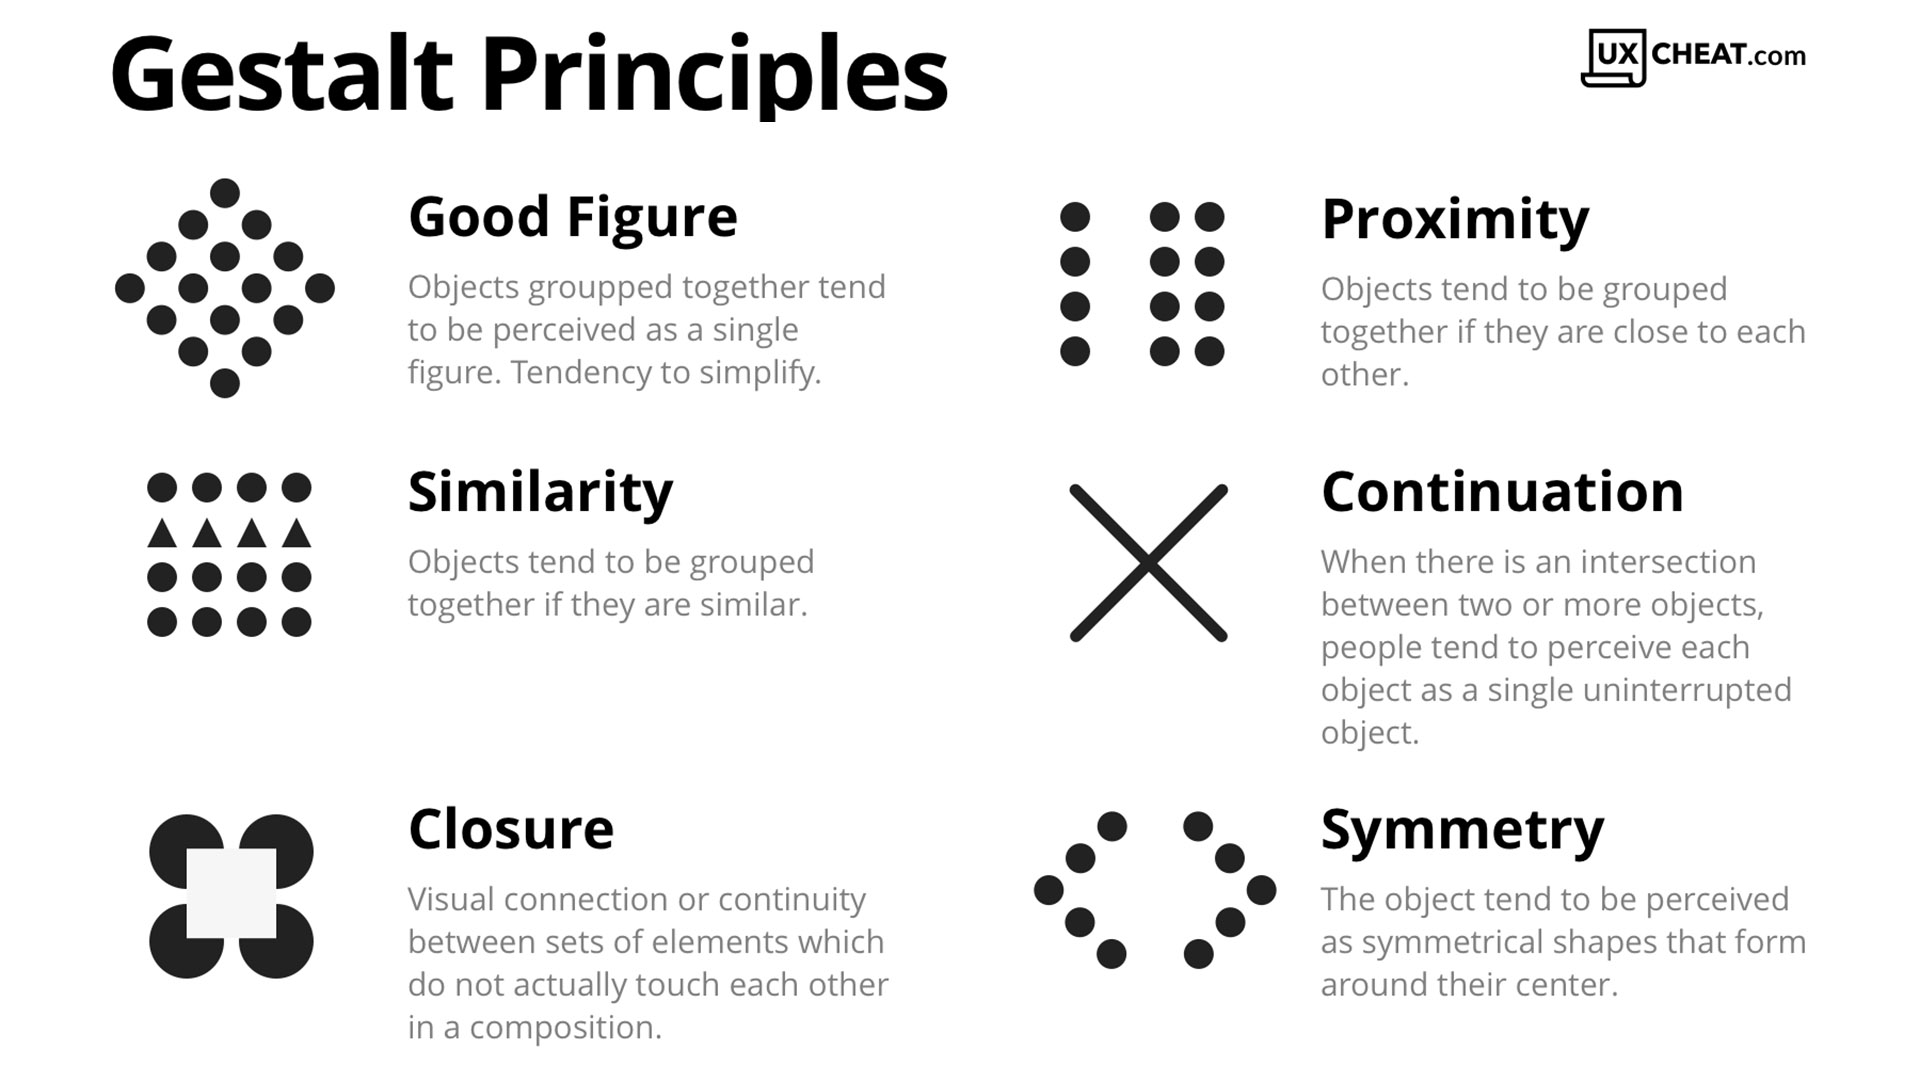
\includegraphics[width=0.75\linewidth]{figure/gestalt_principles} 

}

\caption{Gestalt Principles with Examples}\label{fig:gestalt}
\end{figure}

\db{These principles are based on cognitive psychology and understanding how the human brain processes visual information.}

\db{Eye tracking regression is a method used in eye tracking studies to analyze eye movement data and identify the factors that influence a participant's gaze behavior. 
In eye tracking regression, the eye movement data is regressed on a set of predictor variables, such as visual features of the stimulus or task instructions, to determine the degree of influence each variable has on eye movements.
On the other hand, statistical regression is a technique used in statistics to identify the relationship between a dependent variable and one or more independent variables. 
Statistical regression is used to make predictions or to explain the relationship between variables. 
It is used in various fields, such as economics, psychology, and biology, to analyze and understand complex data.
While both techniques involve regression analysis, they are used for different purposes and with different types of data. 
Eye-tracking regression is specific to eye-tracking data and is used to understand visual attention and perception. 
Statistical regression, however, is a more general technique that can be applied to any type of data and is used for modeling relationships between variables.}

\hypertarget{attention-and-memory}{%
\subsection{Attention and Memory}\label{attention-and-memory}}

Short-term memory (STM), also known as working memory, is the stage of temporary storage and processing where the majority of memory retention effort is expended.
According to (\textbf{baddeley2012?}), STM is a limited-capacity system prone to interference and decay.
Selective attention is essential for the maintenance of STM because it allows us to filter out irrelevant information and concentrate on what is essential Cowan (2001).

Visual aids such as charts and diagrams can improve short-term memory by allowing us to encode and retain information more effectively, according to research (\textbf{alvarez2004?}).

Consequently, utilizing visual aids such as charts can be advantageous for enhancing our short-term memory.

Furthermore, annotations can also be useful in aiding short-term memory.
By adding annotations, such as notes or highlights, to information we are trying to remember, we can improve our recall of the information later on (\textbf{alvarez?}).

According to the Feature Integration Theory (FIT), STM is composed of two stages: pre-attentive processing and focused attention (\textbf{treisman1998?}).
Parallel and independently, the brain processes the physical characteristics of an object, such as its color, shape, and orientation, during pre-attentive processing.
However, focused attention is required to bind these features into a coherent object representation in STM.
STM can be improved through various strategies, such as rehearsal, chunking, and elaboration (\textbf{oberauer2009?}).
For example, by repeating a phone number several times or breaking it down into chunks of two or three digits, we can increase the likelihood of it being stored in STM.
Similarly, by elaborating on the information we want to remember, such as creating mental associations or visual images, we can enhance its retention in STM (\textbf{bui2015?}).

STM is a dynamic and malleable cognitive system that is crucial to our daily lives.
Understanding the mechanisms underlying STM and how to improve it can have significant implications for learning, memory, and the treatment of memory disorders.

\hypertarget{constructing-meaning}{%
\subsection{Constructing Meaning}\label{constructing-meaning}}

Gestalt psychology suggests that humans actively construct meaning by organizing information into patterns and wholes (\textbf{wertheimer1923?}).
Both top-down and bottom-up processing are involved in the process of meaning construction.
Bottom-up processing entails analyzing sensory data from the environment and constructing perceptions based on this data.
Top-down processing is the influence of prior knowledge, expectations, and context on the perception and interpretation of incoming sensory data.

Together, top-down and bottom-up processing facilitate the encoding and retrieval of information in the context of short-term memory.
Selective attention, the ability to focus on relevant information while ignoring irrelevant information, is an example of top-down processing that aids in the encoding and retrieval of information in short-term memory (\textbf{cowan2010?}).\\
According to the feature integration theory, the perception of objects involves both the bottom-up analysis of individual features and the top-down processing of higher-level features in order to form a complete perception (\textbf{treisman1980?}).

The Gestalt principles of perception emphasize the significance of bottom-up and top-down processing in constructing meaning from sensory data.
Both types of processing are involved in encoding and retrieving information, which has significant implications for understanding how short-term memory works.

\hypertarget{expertise}{%
\subsection{Expertise}\label{expertise}}

The development of expertise is a gradual and iterative process that is influenced by numerous psychological factors, such as cognitive processes, automaticity, readily accessible information, and practice effects.

Cognitive Processes - the way we think about and approach a task.

As we become more proficient in a particular skill, we develop more complex and efficient mental models or schemata.
These mental models help us to organize information in a meaningful way, and to quickly identify and solve problems related to the task.
This process is known as cognitive restructuring and is facilitated by developing domain-specific knowledge (\textbf{ericsson1996?}).
For example, a chess master is able to quickly recognize patterns and positions on the board that are common in chess, which allows them to make decisions more quickly and accurately than a novice player.

Automaticity - the ability to perform a task without conscious effort or attention

As our proficiency in a task increases, our performance becomes more automatic, thereby freeing up cognitive resources for other tasks.
The development of procedural knowledge, which is the ability to perform a series of steps or actions in a particular order, facilitates this process (\textbf{Fitts1967?}).
For instance, a skilled typist can type without looking at the keyboard because their finger movements have become automatic.

Information Readily Available - the way we process information related to a task

As our proficiency increases, we can recognize and retrieve pertinent information more rapidly and precisely than a novice.
This is made possible by the creation of domain-specific knowledge structures that allow us to retrieve pertinent information from memory quickly (\textbf{Chase1973?}).
For instance, a medical expert can quickly identify signs and diagnose a patient using their knowledge of disease symptoms and risk factors.

Practice Effects - extensive practice and experience

Practice effects are the performance enhancements that result from repeated practice.
These gains are frequently most significant at the outset of practice, but gradually diminish as the individual approaches their performance ceiling (\textbf{Anderson1982?}).
The development of procedural knowledge and automaticity, which allow for more efficient and accurate task performance, facilitates the effects of the practice.

\hypertarget{engagement-with-the-data}{%
\subsection{Engagement with the data}\label{engagement-with-the-data}}

\db{
The goal of data analysis is to extract meaningful insights, patterns, and knowledge from data. 
The process of data analysis involves collecting, cleaning, transforming, and modeling data, followed by the use of statistical and machine learning methods to uncover patterns and relationships within the data. 
The end goal of data analysis is to support decision making and provide a basis for informed action. 
Data analysis can help organizations to better understand their customers, market trends, and operational performance. }

\db{Additionally, data analysis can support scientific research by helping researchers to test hypotheses, develop theories, and gain a deeper understanding of complex phenomena. 
Ultimately, data analysis aims to turn data into actionable insights and information that can inform and improve decision-making.}

\hypertarget{data-considerations}{%
\section{Data Considerations}\label{data-considerations}}

Grammar allow us to separate data type from rendering

\db{Frame as a way to easily change between appropriate forms of presentation for a given variable or set of variables.}

It doesn't help us decide which is better - for that we need user testing.

In the field of graphical communication, semiology, or the study of signs and symbols and their use in communication, has been a valuable tool.
One of the fundamental principles of semiology is the relationship between signifier and signified, in which a visual element (the signifier) represents a particular meaning or concept (the signified) ((\textbf{Barthes1972?})).
Another essential concept in semiology is the utilization of syntax and semantics to effectively convey meaning in graphic communication.
This includes both the syntax and semantics of a graphic's visual elements ((\textbf{Bertin1983?})).

The use of color to represent data on maps is an example of successful graphical communication utilizing semiology.
By using different colors to represent different data points, viewers can comprehend patterns and relationships in the data quickly and easily.
Jacques Bertin (1983) writes in ``Semiology of Graphics'' that color can be used to ``emphasize a point, distinguish one category from another, or establish a relationship between two points.''
In addition, Bertin explains that the use of color can help overcome language barriers, making it easier for the audience to comprehend the presented information.

Graphs are another tool that can be used to effectively communicate information via semiology.
By utilizing visual elements such as bars and lines to represent data, graphs can make complex information more understandable to viewers.
For instance, a line graph can be used to illustrate the change in value of a stock over time, making it easier for investors to identify trends and patterns. Leland Wilkinson ((\textbf{wilkinson2012?})) writes in his book ``The Grammar of Graphics'' that ``graphical methods are not only superior to other forms of communication, but also superior to numerical or verbal methods for certain types of data and reasoning.''

\db{It proposes that any statistical graphic can be broken down into a set of essential components, or "grammar," that can be combined in different ways to create a wide range of visualizations, following a layered approach to describe and construct visualizations or graphics in a structured manner.}

The components of the grammar of graphics include:

\begin{itemize}
\tightlist
\item
  Data: The raw data being visualized represents a set of observations or values.
\item
  Aesthetic Mappings: The mapping of data variables to visual properties such as position, color, shape, and size.
\item
  Scales: The mapping of data values to visual values, such as mapping a numerical value to a bar height.
\item
  Geometries: The basic shapes representing the data, such as points, lines, bars, and histograms.
\item
  Facets: The plot division into multiple subplots, each representing a different subset of the data.
\end{itemize}

\db{For example, a bar chart can be created by mapping a categorical variable to the x-axis, mapping a numerical variable to bar heights, and using rectangular bars as the geometry. 
For example, mapping two numerical variables can create a scatter plot to the x and y positions and use points as the geometry.
Finally, the Grammar of Graphics provides a systematic way of thinking about visualizations, making it easier to choose the appropriate visual representation for a given dataset.
}
\begin{figure}

{\centering 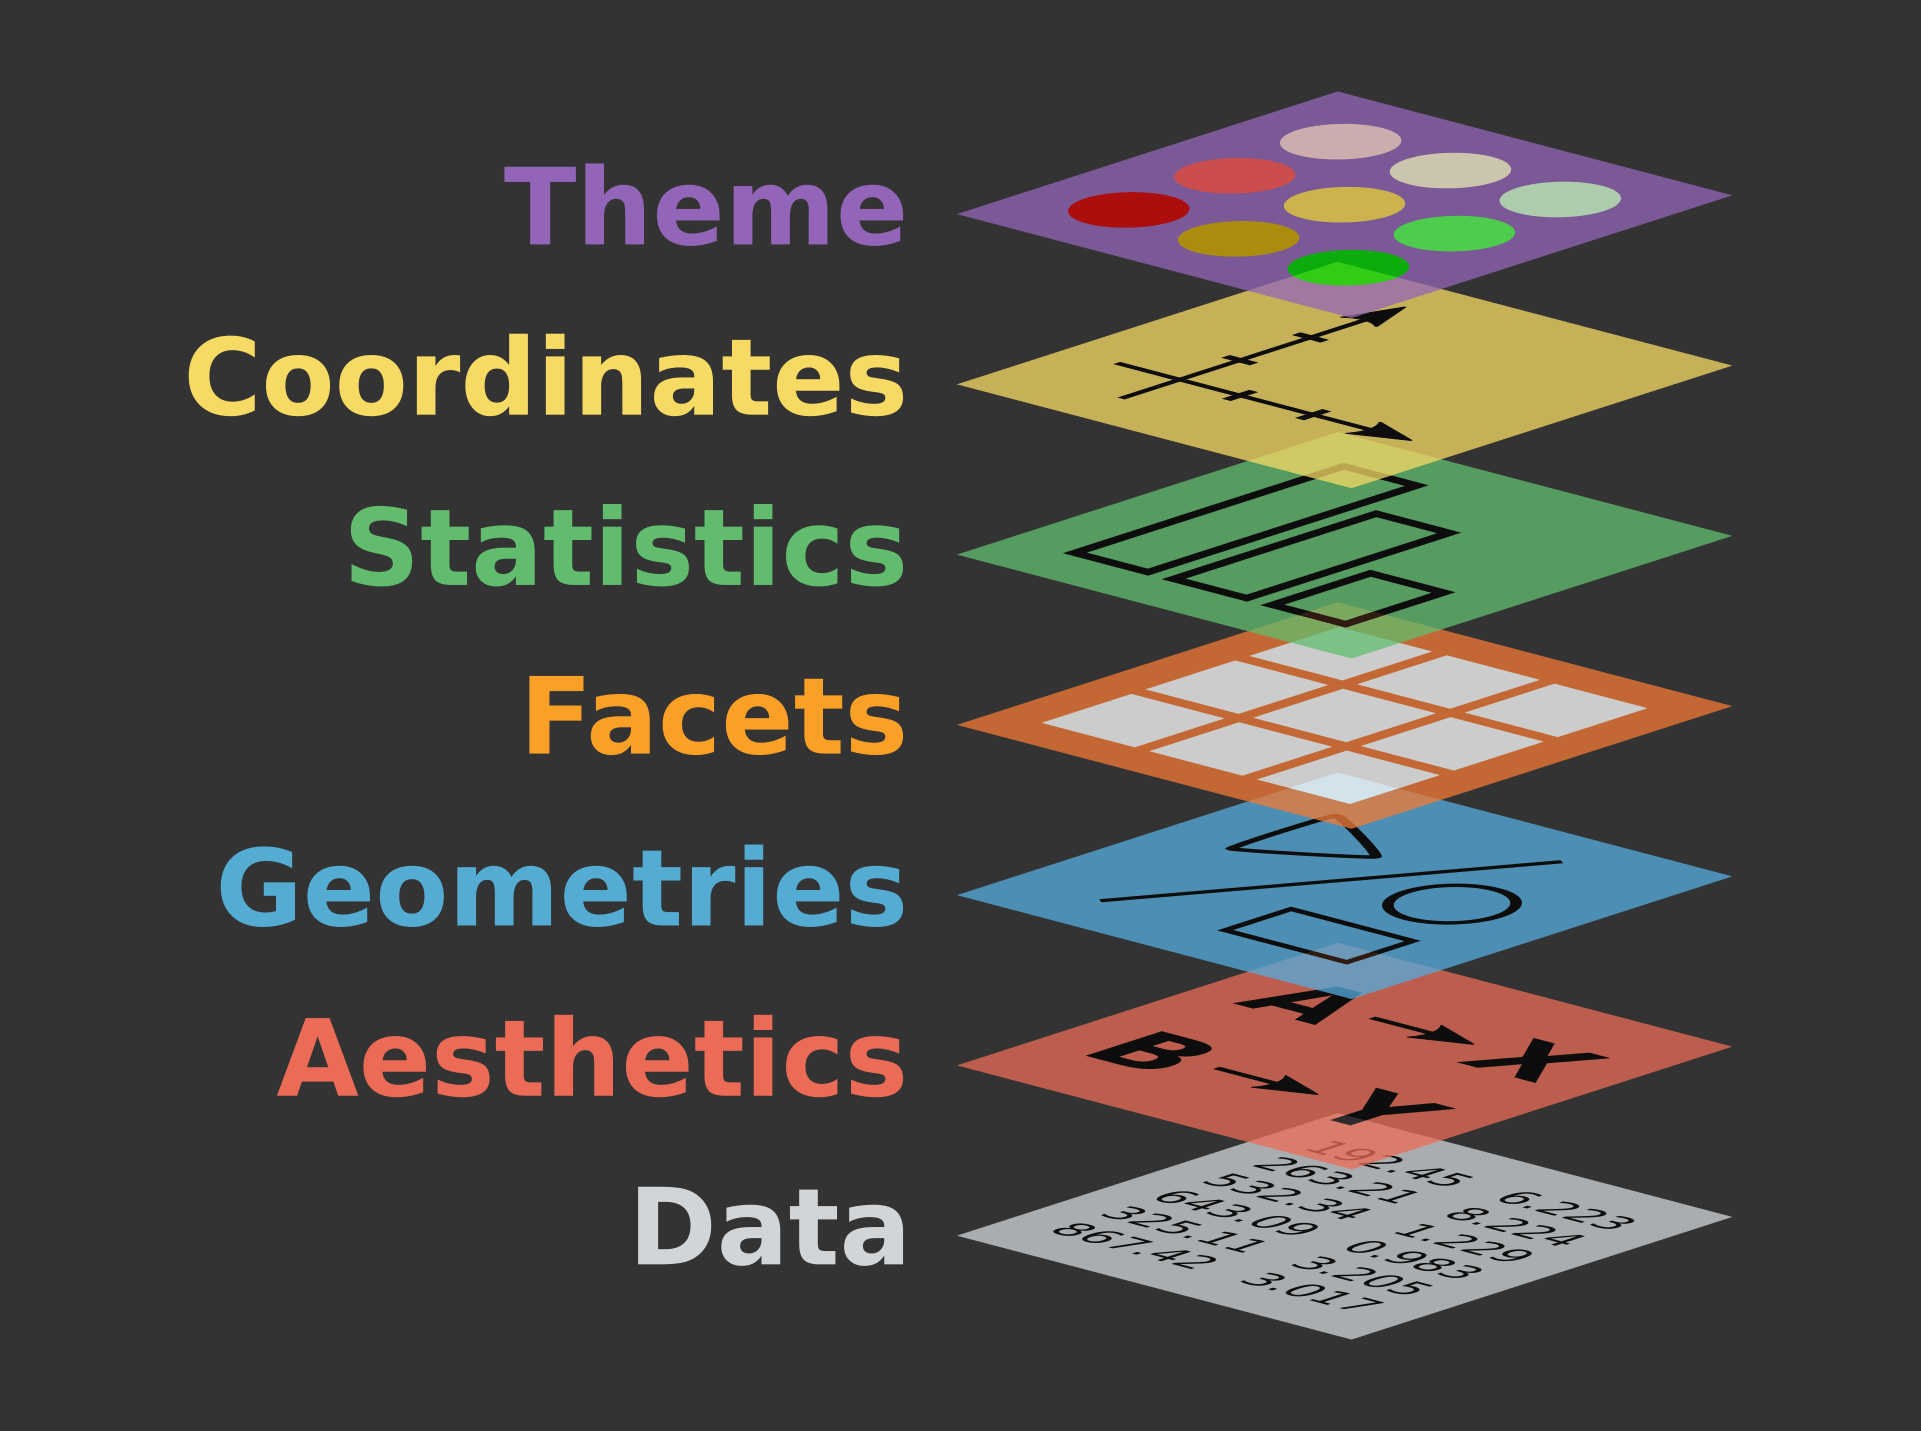
\includegraphics[width=0.45\linewidth]{figure/gglayers} 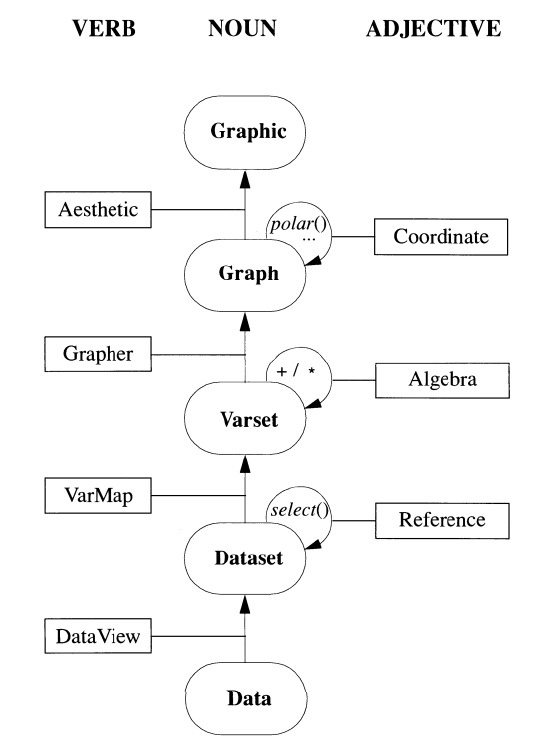
\includegraphics[width=0.45\linewidth]{figure/graphic-flowchart} 

}

\caption{Grammar of Graphics Diagram of Wickham and Wilkinson's work}\label{fig:graphics2}
\end{figure}

The application of semiology in graphical communication is not devoid of obstacles.
One difficulty is the possibility of misinterpretation, in which viewers may assign a different meaning to a visual element than was intended ((\textbf{Bertin1983?})).
Another concern is the possibility of cultural differences in interpretation, in which a visual element may have a different meaning in one culture versus another ((\textbf{Norman2013?})).

Despite these obstacles, semiology in graphical communication remains an indispensable tool for effectively conveying information.
By understanding semiology principles and syntax and semantics' role in graphical communication, designers can create compelling visual representations that convey information clearly and concisely.

Michael Friendly has investigated the origins and development of graphic techniques, tracing their evolution from antiquity to the present.
\db{Friendly detailed using SAS with hands-on experiments to present categorical data analysis visually @friendly2014.}
By emphasizing the role of graphical methods in scientific discovery, Friendly has helped promote his use in various disciplines, from the natural sciences to the social sciences and beyond.
In his book ``Milestones in the History of Thematic Cartography, Statistical Graphics, and Data Visualization,'' Friendly (2019) provides a comprehensive overview of the key milestones in the evolution of statistical graphics, including the contributions of pioneers like William Playfair, Charles Minard, and John Tukey.

\db{John Tukey was the first to organize the collection and methods associated with philosophy into Exploratory Data Analysis (EDA). 
John Tukey, creator of stem-and-leaf plot, boxplot-resistant smooth, and the violin plot (also known as rootgram) who taught us to utilize these methods to organize and demonstrate EDA. 
He was a strong advocate for the importance of EDA as a crucial first step in the data analysis process and emphasized the need for visualization and interactive techniques to understand patterns and relationships in data.}

\begin{center}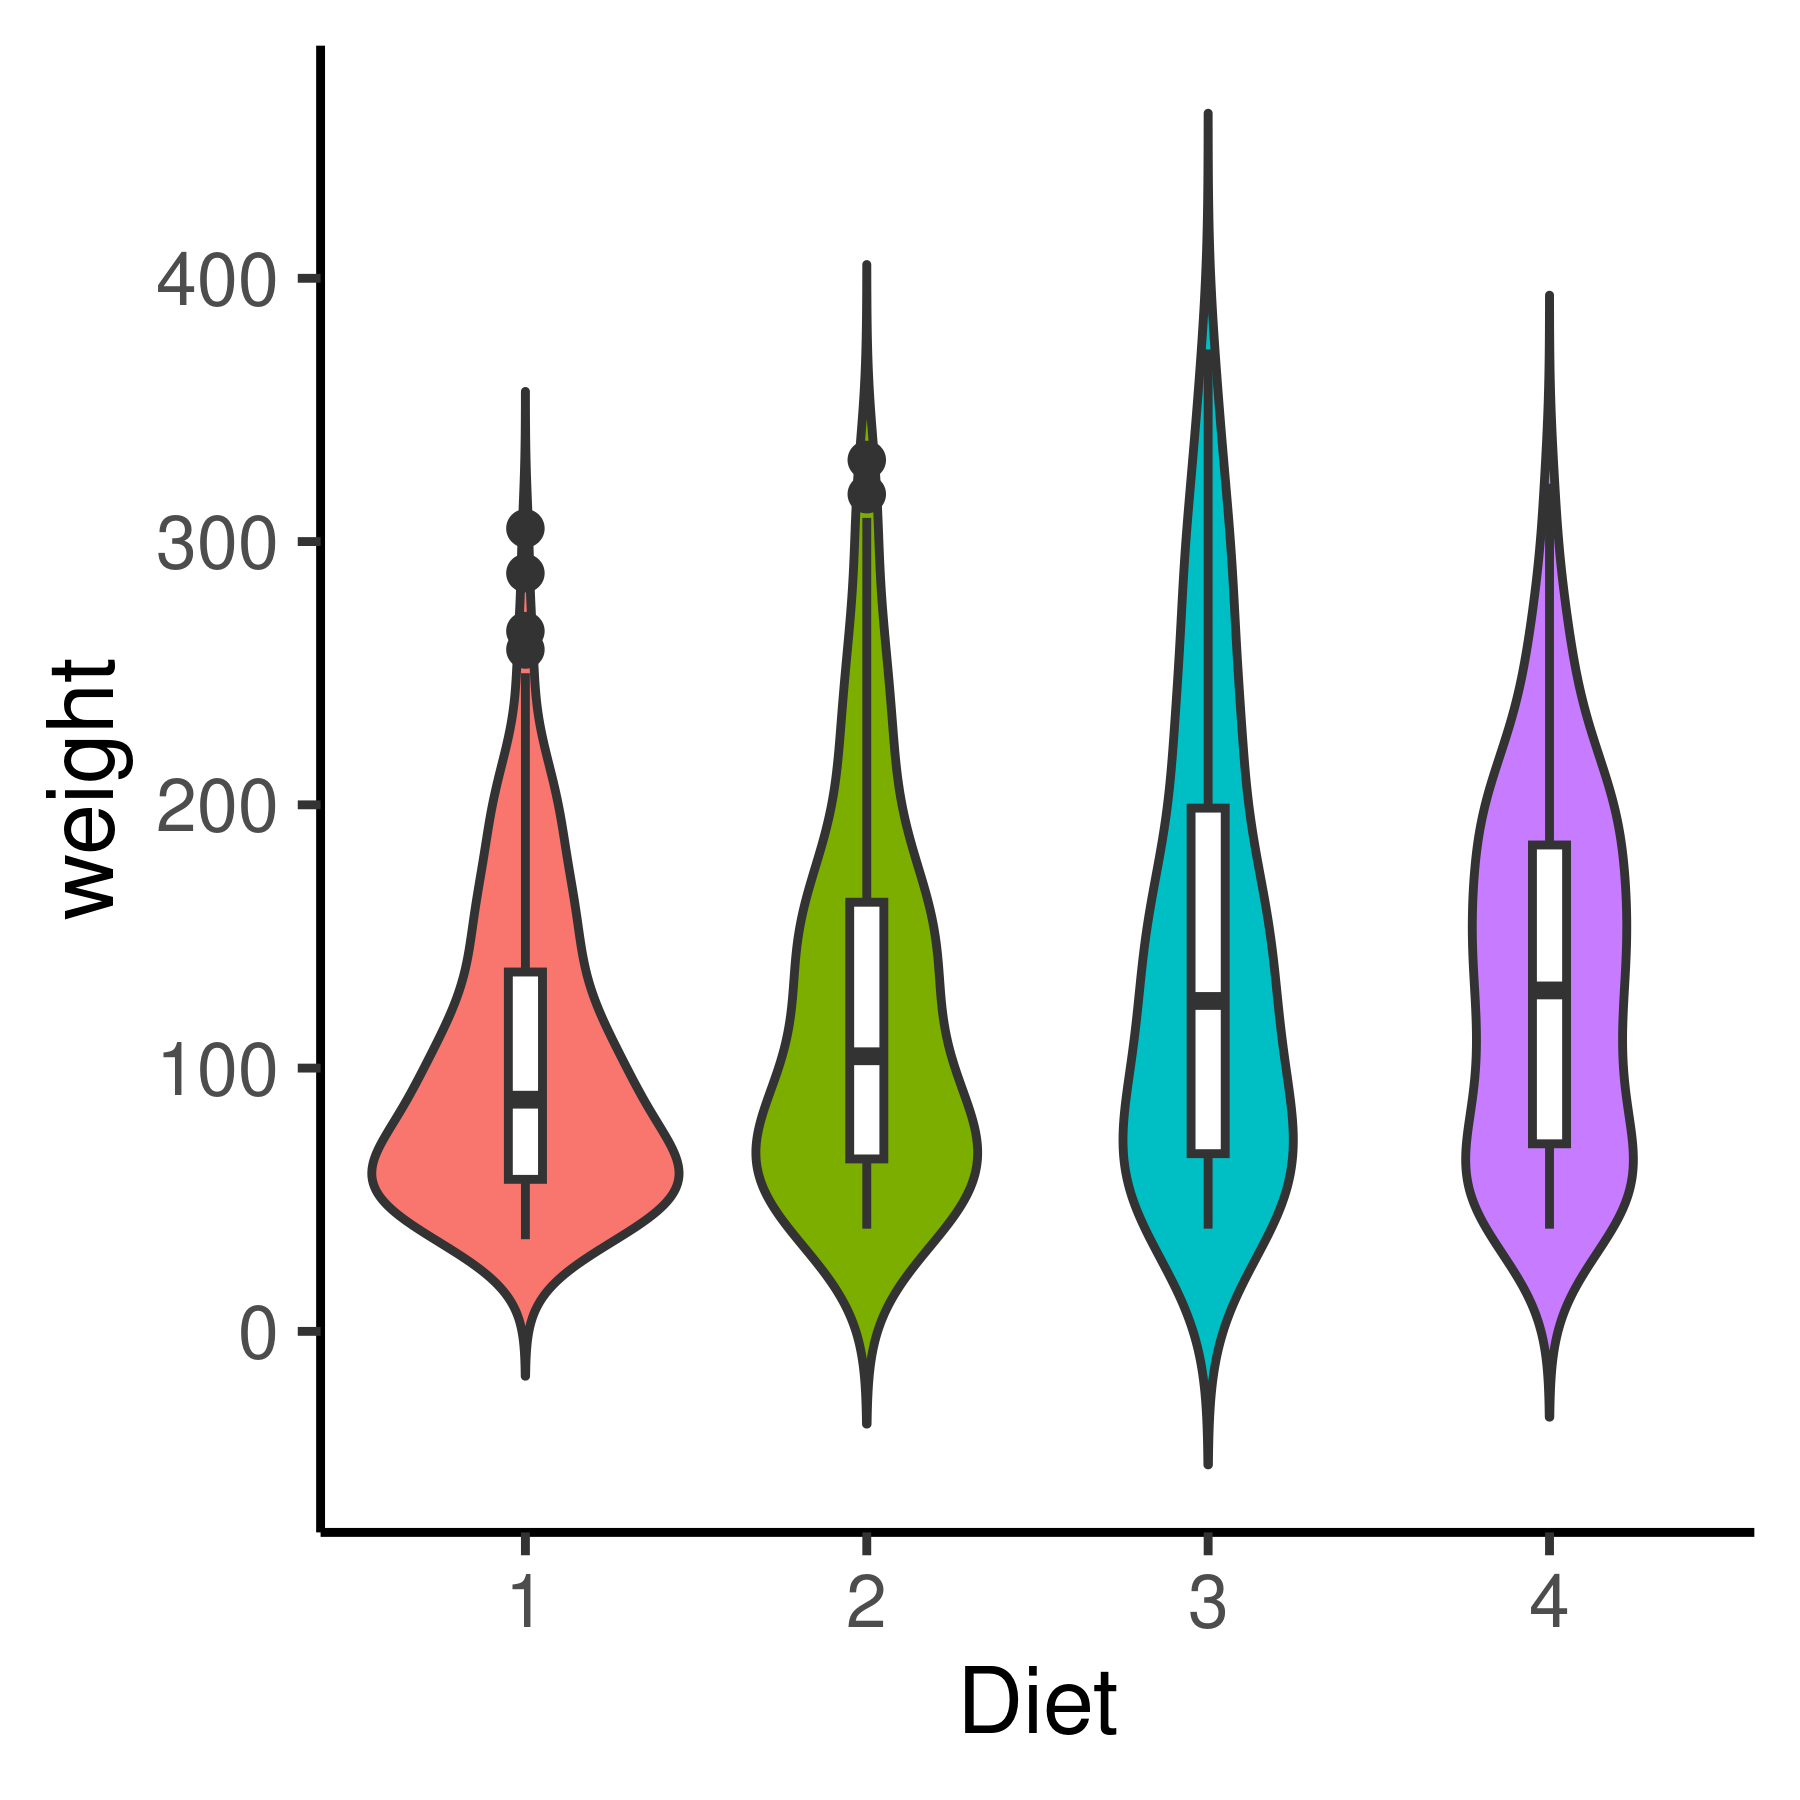
\includegraphics[width=.49\linewidth]{thesis_files/figure-latex/violin_plot-1} 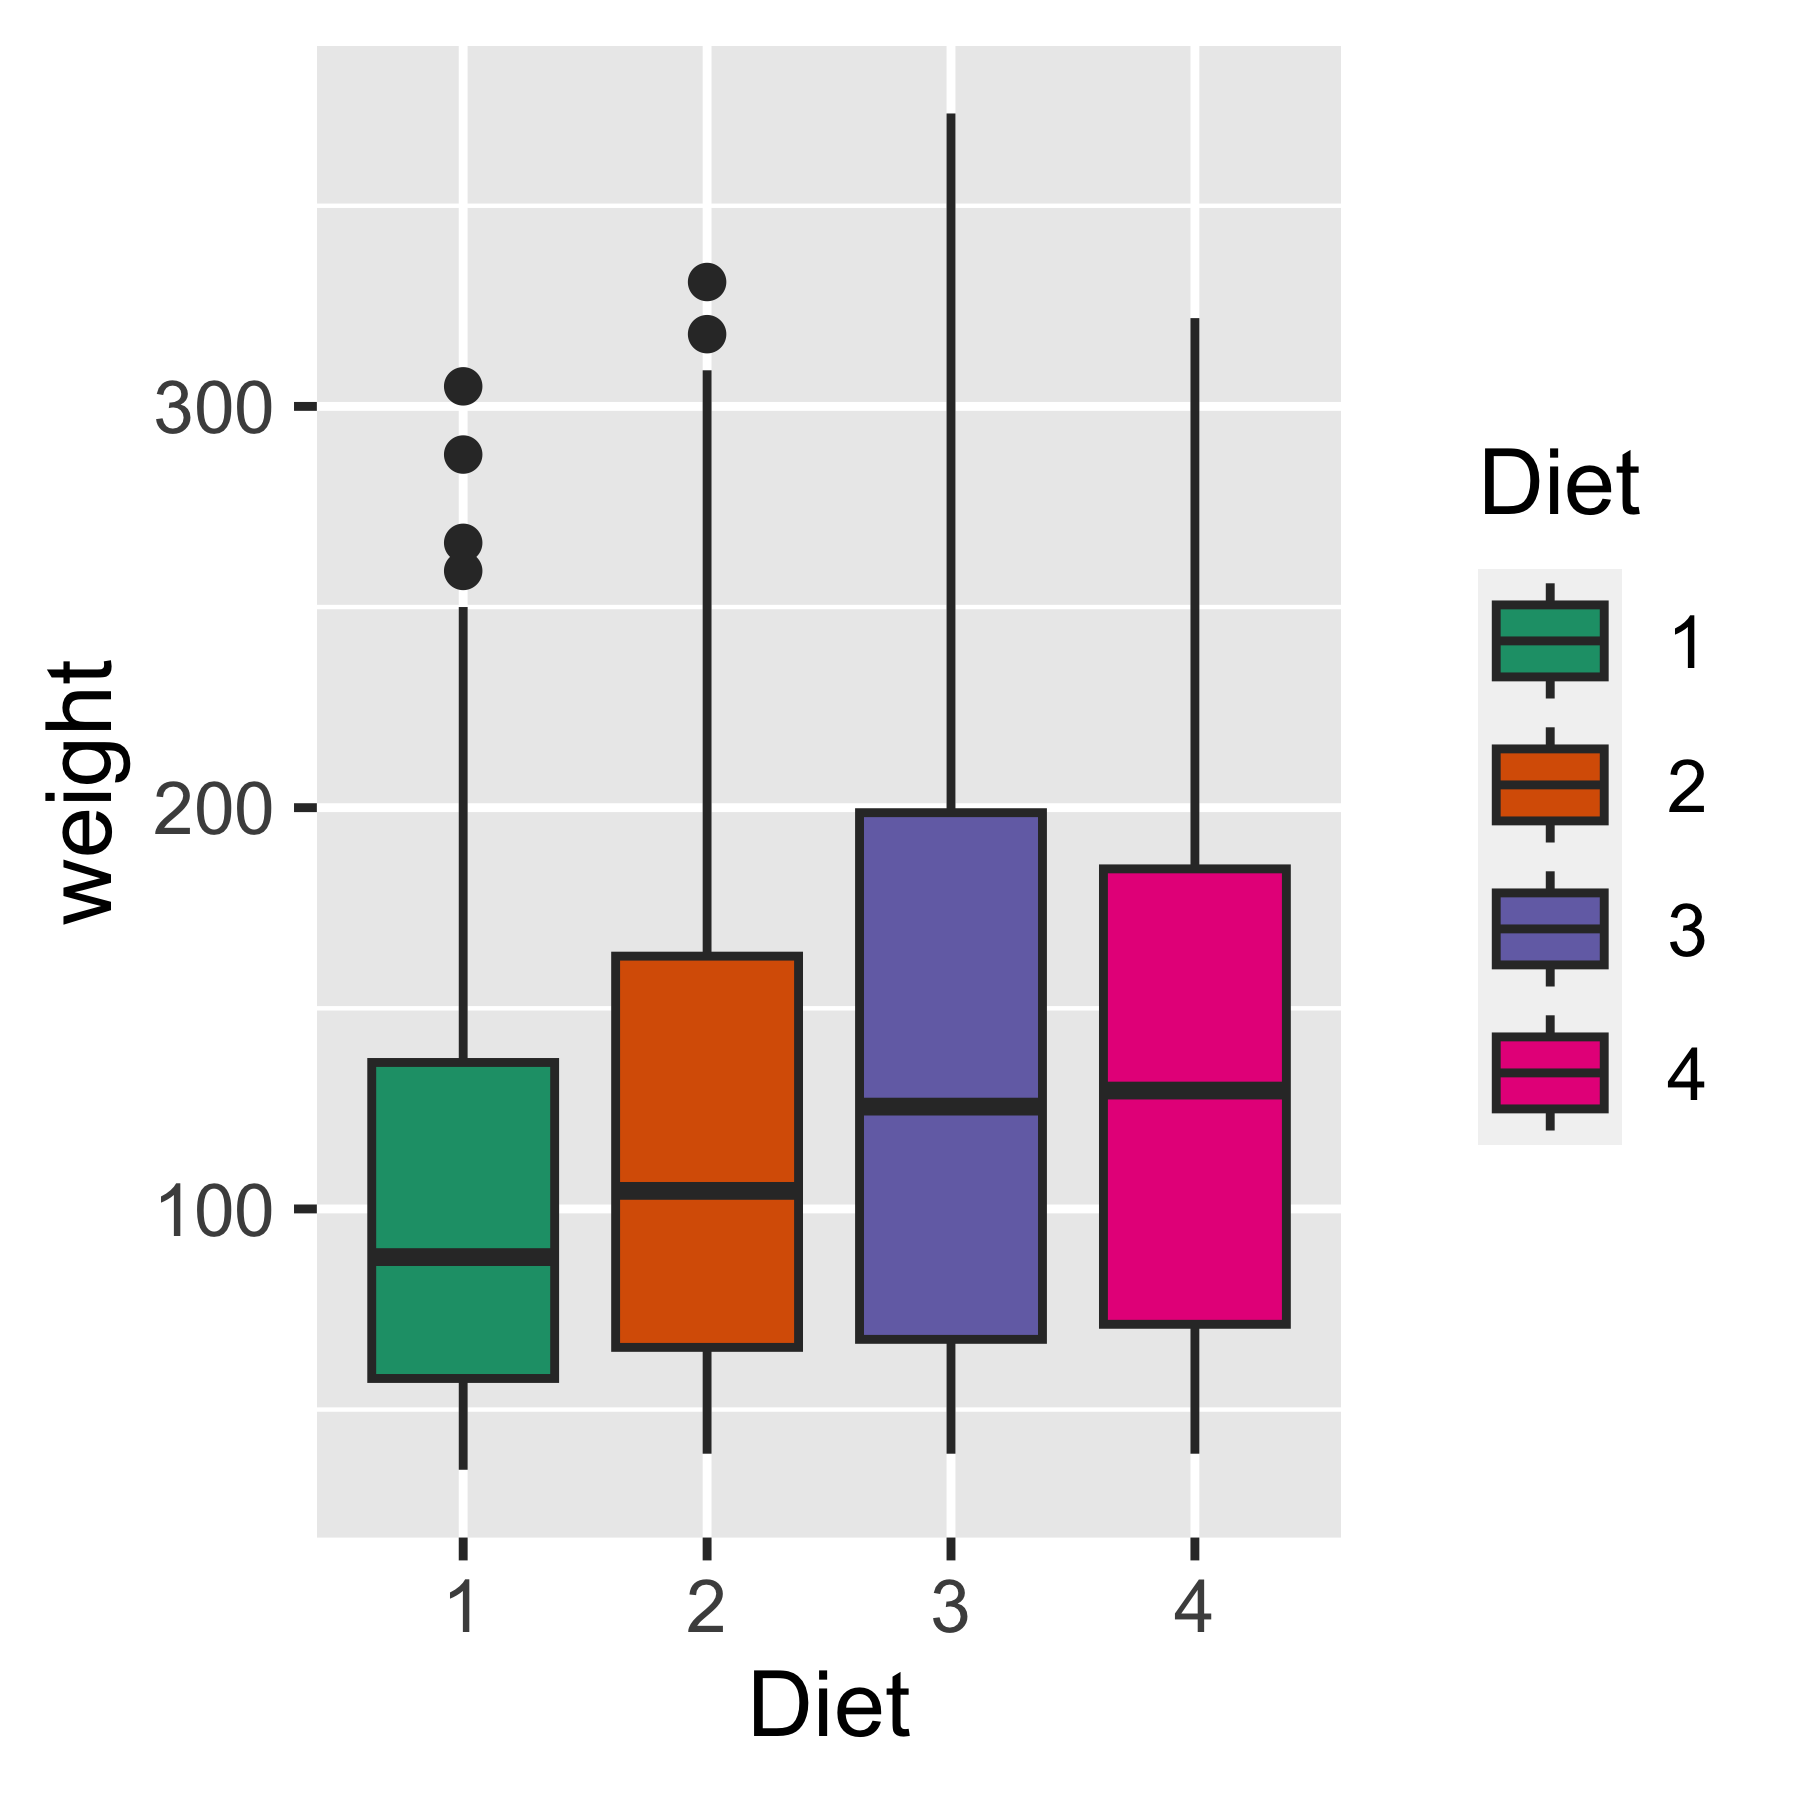
\includegraphics[width=.49\linewidth]{thesis_files/figure-latex/violin_plot-2} \end{center}

\db{Tukey's Principles in EDA:}

\begin{enumerate}
\def\labelenumi{\arabic{enumi}.}
\tightlist
\item
  Graphical exploration looking for patterns or displaying fit.
\end{enumerate}

\begin{itemize}
\tightlist
\item
  The method demonstrates things about data that are not understood by a single numeric metric.
  This has been useful in graphing the data before you develop summary statistics.
\end{itemize}

\begin{enumerate}
\def\labelenumi{\arabic{enumi}.}
\setcounter{enumi}{1}
\tightlist
\item
  Describing the general patterns of the data.
\end{enumerate}

\begin{itemize}
\tightlist
\item
  This step should be insensitive to outliers.
  In general, think about the types of resistant measures (i.e., median or mean).
  This step is making sure to determine data patterns.
\end{itemize}

\begin{enumerate}
\def\labelenumi{\arabic{enumi}.}
\setcounter{enumi}{2}
\item
  The natural scale/state that the data are at their best.
  This will be the step at which the scale of data can be helpful for analysis.
  The reexpressing data to a new scale by taking the square root or logarithmic scale.
\item
  The mostly known parts of EDA but is done in the way of accessing fit of the data.
  This is taught in every statistics 101 class.
  The growth of machine learning and prediction methods have now used residuals more in the toolbox to assessing the best prediction models.
\end{enumerate}

\begin{itemize}
\tightlist
\item
  The idea generally is to determine the deviations in the data from a general pattern by looking at the data from the fit of the data.
\end{itemize}

\db{Visualizations of data are essential for exploratory data analysis (EDA) along with model diagnostics. 
Plots for EDA are a valuable tool for guiding an analyst in discovering the relationships between variables in their data. 
When using plots in model diagnostics, plots help analysts determine whether or not the model is an appropriate way to model. 
During the initial EDA stage, an analyst may find that a variable or a covariate is directly related to the dependent variable when looking at a correlation heatmap or a scatterplot. 
This will be important to know before starting a linear model analysis. 
Much of our general understanding is from introductory statistics courses. 
The basic understanding can be formalized to visualize the discovery process.}

Effective graphics can be a powerful tool for communicating complex information, which makes numerical accuracy, engagement, correct decision-making, and accurate predictions crucial considerations.
In this summary, we will examine key strategies for creating better graphics that meet these criteria, based on recent research findings.

\db{Static Visualization is commonly used in the communication phase of data science workflows, and data scientists sometimes use them as part of the analysis. 
John Tukey's EDA methods are currently known and well-vetted in the field. 
However, Satyanarayan et. al began to address this by introducing a high-level grammar of graphics called "Vega-Lite," which presents a set of standardized linguistic rules for producing interactive information visualizations using a concise JSON format for data to be represented by the grammar [@satyanarayan2016]. 
Vega-Lite has been directly implemented in R via the `ggvis` package using the same - albeit slightly lower-level.}

\begin{verbatim}
## Warning: Groups with fewer than two
## data points have been
## dropped.
\end{verbatim}

\begin{verbatim}
## Warning: Removed 1 rows containing
## missing values
## (`position_stack()`).
\end{verbatim}

\begin{verbatim}
## `stat_bin()` using `bins =
## 30`. Pick better value with
## `binwidth`.
\end{verbatim}

\begin{center}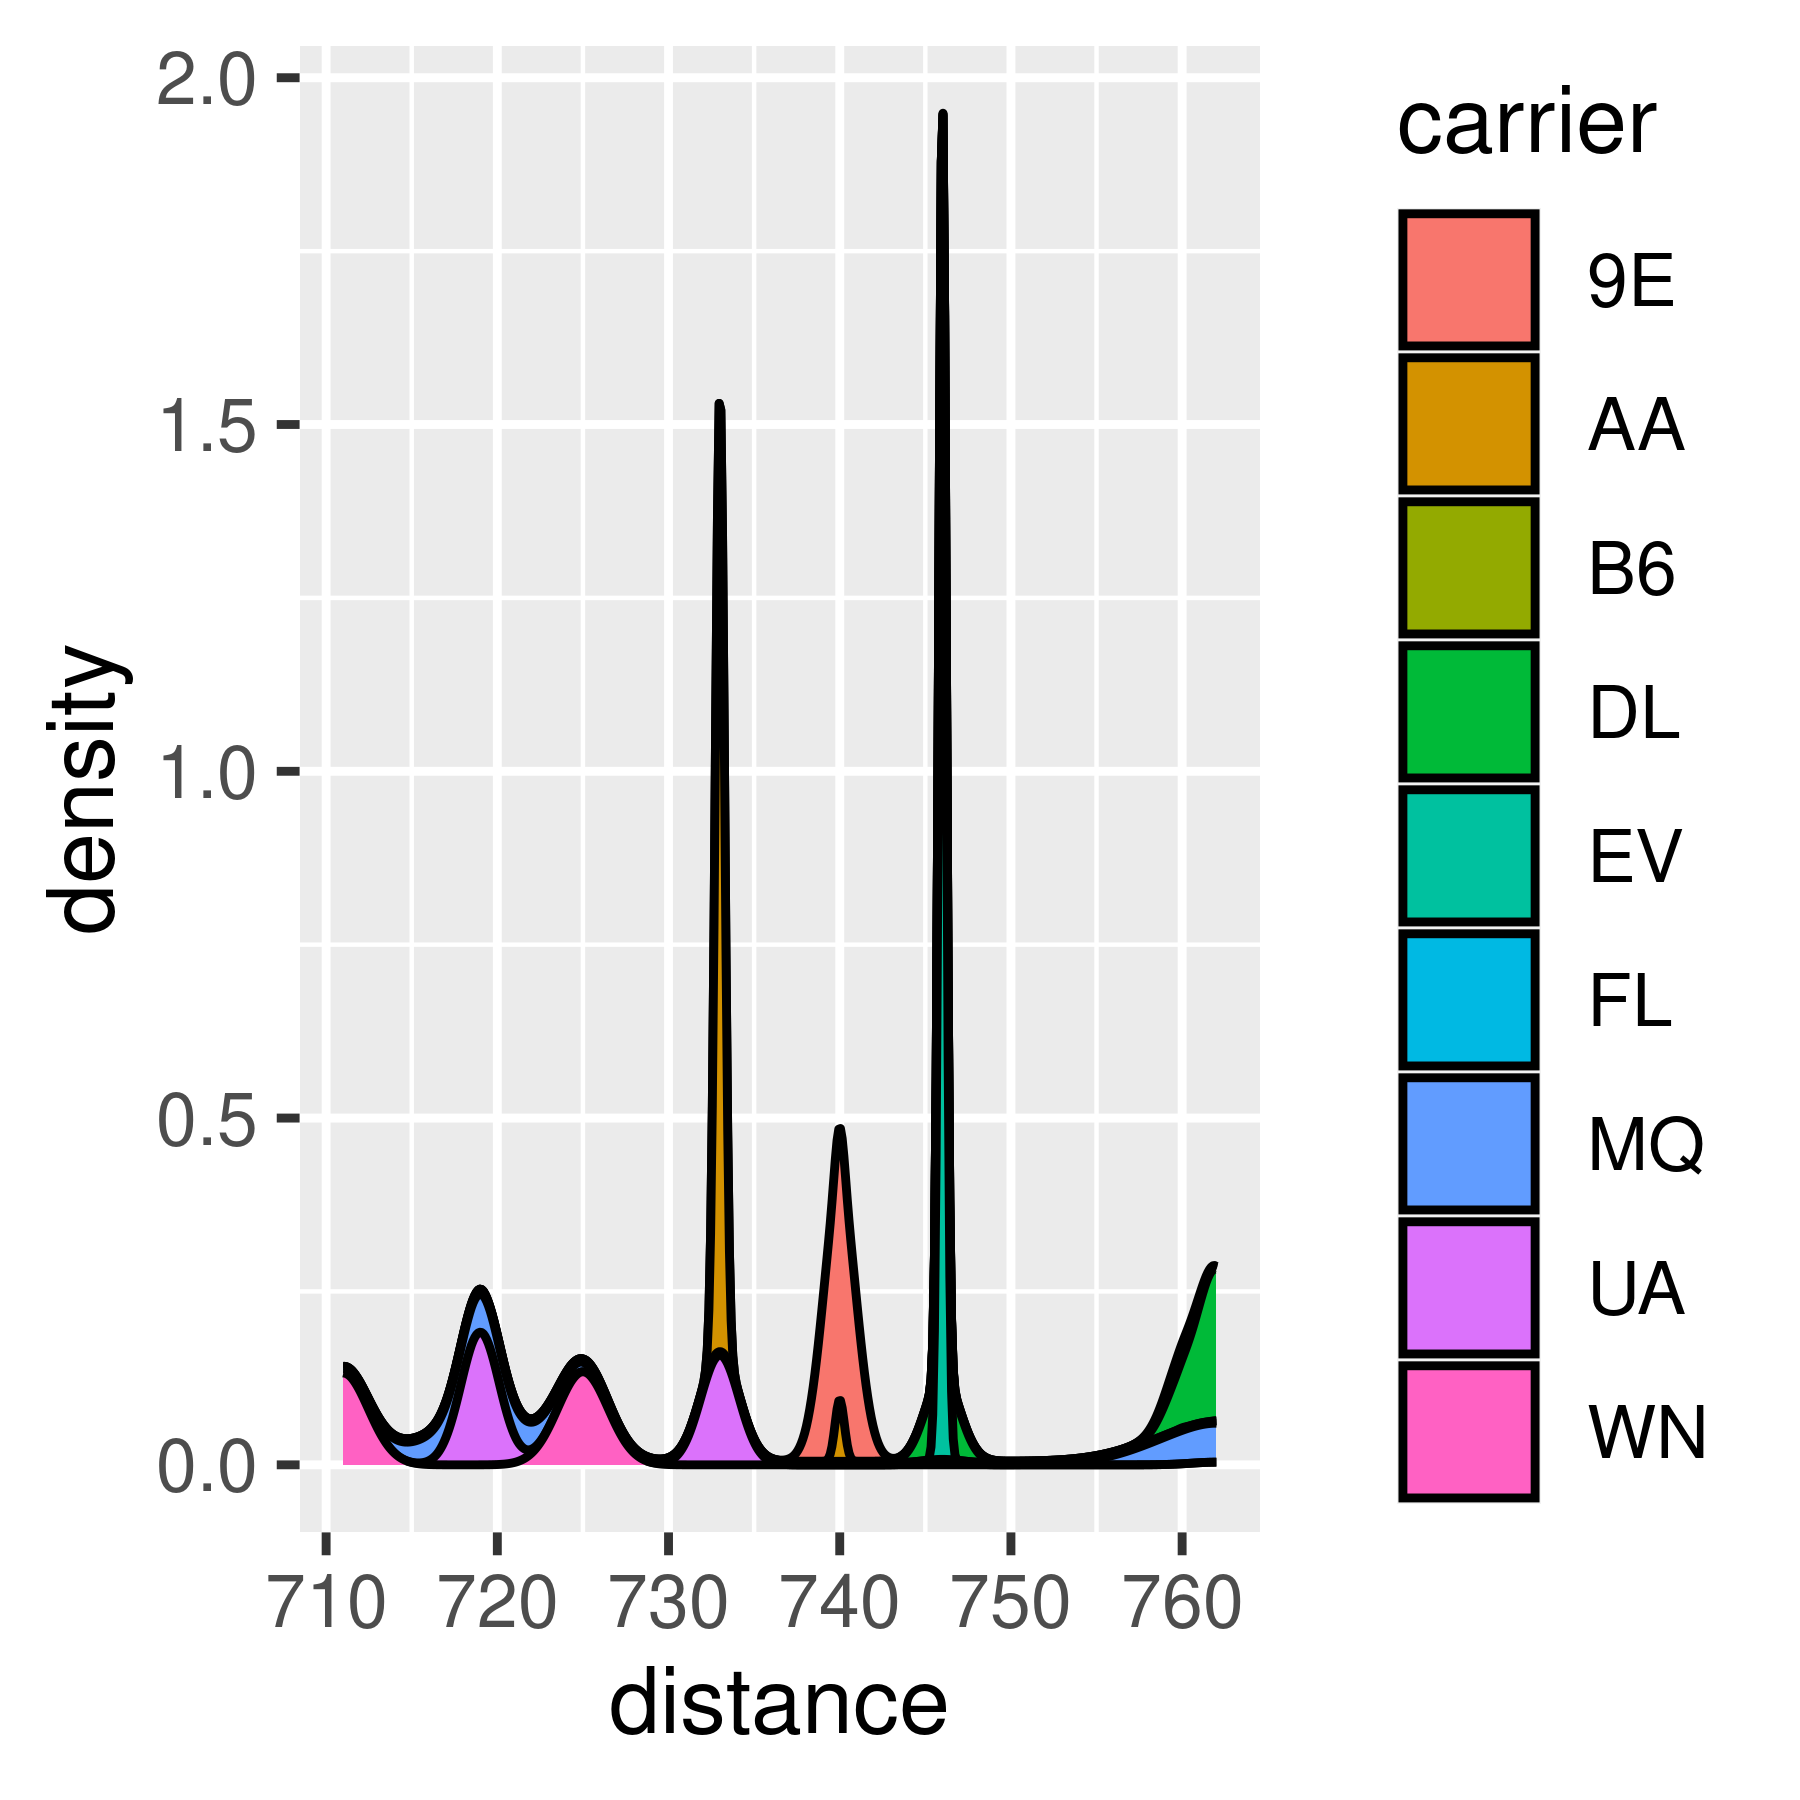
\includegraphics[width=.49\linewidth]{thesis_files/figure-latex/flights_data_example-1} 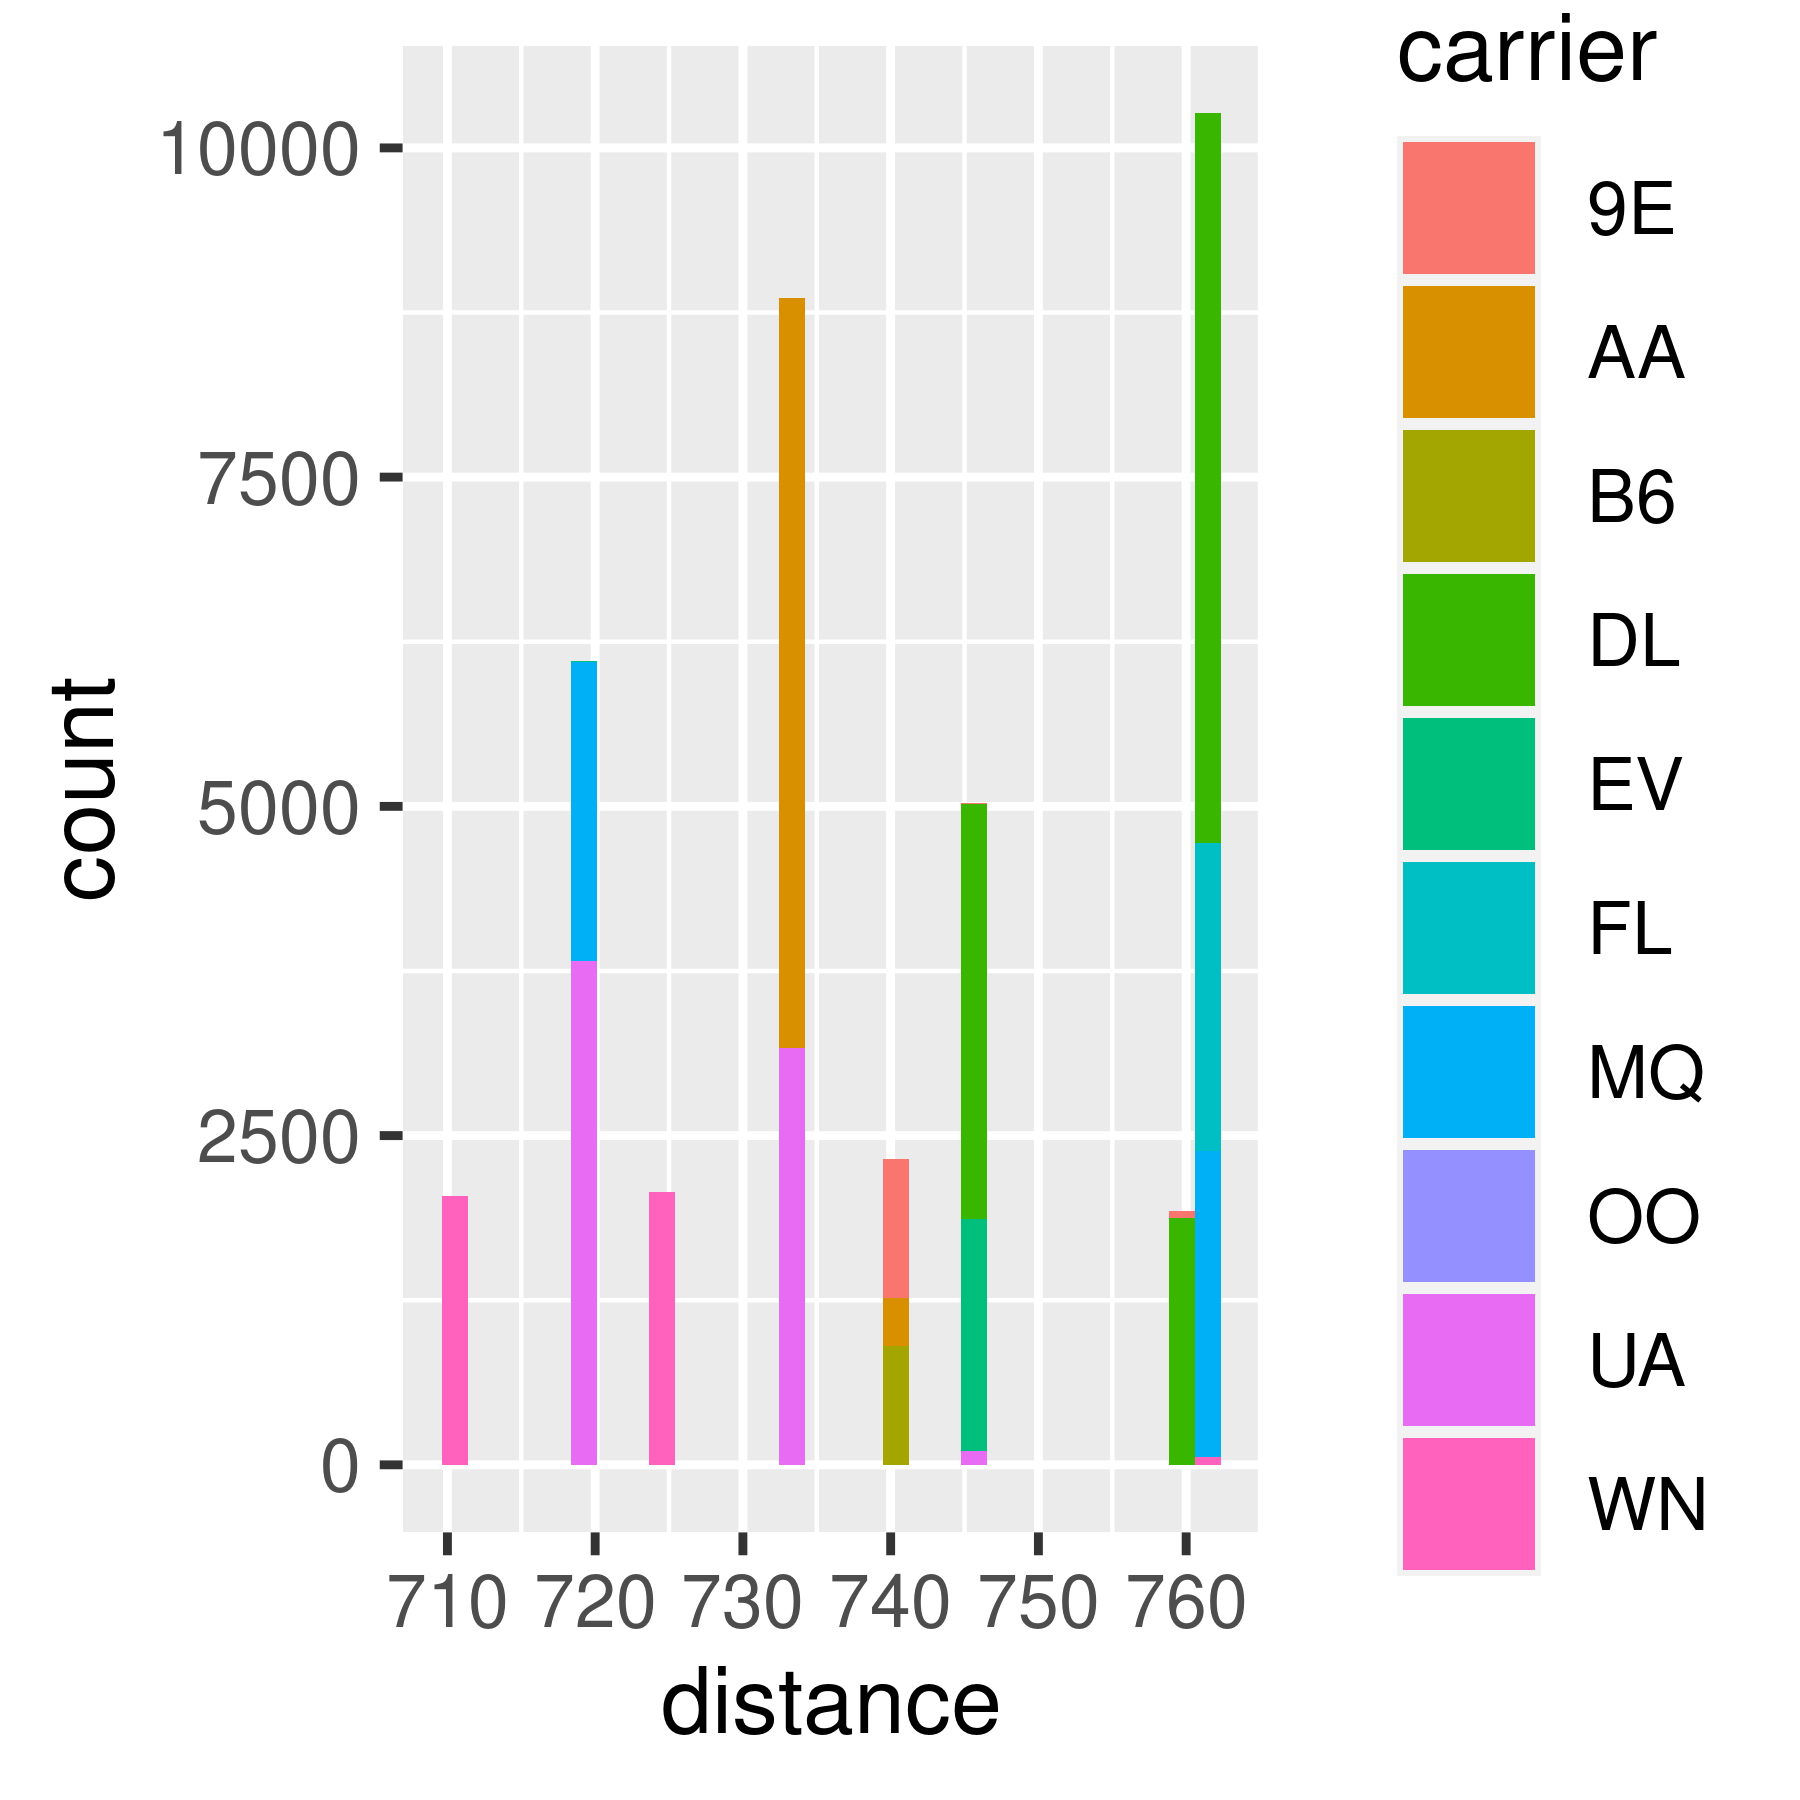
\includegraphics[width=.49\linewidth]{thesis_files/figure-latex/flights_data_example-2} \end{center}

\db{On the other hand, Dashboards are interactive interfaces that display data visually to provide insights and support decision-making. 
Dashboards can be used to monitor key performance indicators, track progress over time, and identify patterns and trends in data. 
They often display real-time data and can be customized to show the most relevant data to the user.}

\hypertarget{interactive-graphics}{%
\subsubsection{Interactive Graphics}\label{interactive-graphics}}

\db{The area of interactive graphics is still very much a work in progress despite existing as a field of research since the late 1960s—developments are driven partly by new technology, such as `d3` [@bostock2011]. 
Visualizations are more than just a picture. 
They are now a tool that facilitates analytic activity through different modes of interaction [@yi2007]. 
Visualization is context-free, as it can mean different things to different people depending on the situation [@parsons2014]. }

\db{Interactive graphics, are essential to EDA [@unwin1999]. 
Beyond the limitations of static statistical displays, interactive graphics enable visualizations to advance alongside the analysis. 
User interaction and direct manipulation are required for dynamic graphics to reach their full potential (@cook1995; @unwin1999).
The connection between EDA and dashboards is that EDA is the process of preparing and understanding the data, which is the first step for building a dashboard, as the data has to be cleaned, transformed, and analyzed to be used efficiently on the dashboard. 
EDA results can be used to identify the most relevant data and metrics to include in the dashboard and to design the visualizations that will be used to display the data. 
And also, the EDA process can be used to identify the outliers, patterns, trends, and insights that will be useful to show in the dashboard to support decision-making.}

\db{The van Wijk Simple Visualization Model is a diagrammatic representation that provides a simple and effective way to understand and visualize the flow of information and data through a system. 
It is a commonly used tool in Exploratory Data Analysis (EDA), which is the initial step in the data analysis process. 
The van Wijk model can be used to represent the flow of data from data sources, through intermediate processing stages, to the final visualization of results. 
van Wiij's simple visualization model shows how insights are generated as the human participates in a feedback loop between reading and interacting with visualization [@van2005]. }

\db{This model is also context-free, allowing for the focus to be on the feedback loops between visualization and the user.}

\db{The relationship between the van Wijk Simple Visualization Model and Human-Computer Interaction (HCI) lies in the area of data visualization. 
The van Wijk Model provides a framework for understanding how information and data flow through a system to be displayed to the user. 
In the context of HCI, the model helps to understand how data is processed, transformed and presented to the user in a way that is intuitive, informative and engaging. 
The model helps to identify the various steps involved in the visualization process, from the collection and processing of data to the presentation of results. 
By doing so, it supports the design of more effective and user-friendly visualizations, which can enhance the overall user experience.}

\begin{center}
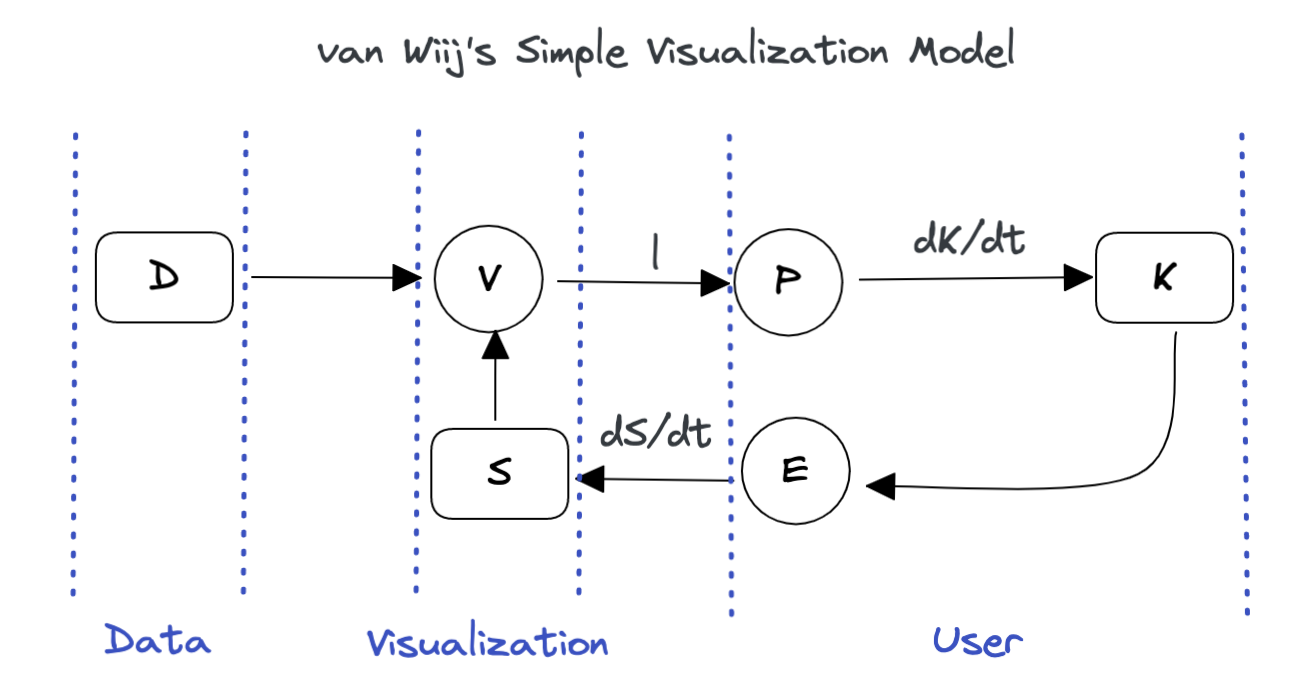
\includegraphics[width=\textwidth]{figure/vanWiijSimpleModel.png}
\captionof{figure}{van Wiij Simple Visualization Model}
\end{center}

\db{Interaction allows the user to define what data they see and how they see it, creating a dialogue between the user and the system. 
Theories behind visual representation include:}

\begin{itemize}
\tightlist
\item
  graphical comprehension ((Cleveland \& McGill, 1984))
\item
  preattentive processing ((Ware, 2012))
\item
  gestalt theory ((Few, 2009))
\item
  graphical excellence ((\textbf{tufte2001?}))
\end{itemize}

Theories behind the manipulation of visualizations include but are not limited to:

\begin{itemize}
\tightlist
\item
  cognitive fit ((Vessey \& Galletta, 1991))
\item
  visual perceptual approaches ((\textbf{baker2009?}))
\item
  human information processing
\end{itemize}

\db{As interactive visualizations play a more significant role in information systems, designers must know what tasks, visual representations, and interaction techniques are available and how they work to facilitate analytical reasoning. 
They must decide on the most effective visual representation without being able to estimate every user's ability to read and interpret the visualization.}

\db{The human brain can only take in a set amount of data from a table or a paragraph.} \svp{references?}

\hypertarget{audience-data-interactions}{%
\section{Audience-Data Interactions}\label{audience-data-interactions}}

\db{User analysis is a crucial step in the design of user interfaces, especially in Human-Computer Interaction (HCI) and User Experience (UX) design. 
It involves studying the users of a system to understand their needs, goals, and behaviors. 
The purpose of user analysis is to create interfaces that are easy to use, efficient, and effective for the intended audience.
The results of user analysis can be used to inform the design of the interface, including the layout, navigation, and functionality. 
It can also be used to identify areas of the interface that are confusing or difficult to use and to make recommendations for improvements. 
User analysis is an iterative process, and it should be done in multiple stages of the design process to ensure that the final product is tailored to the users' needs.}

\hypertarget{background-on-static-graphics}{%
\subsection{Background on static graphics}\label{background-on-static-graphics}}

Cleveland and McGill investigated the effect of various bar chart designs on the accuracy with which viewers perform simple perceptual tasks (\textbf{Cleveland?}).
People perform significantly worse on stacked bar charts than on simple bar charts, and bar charts with filled bars are generally superior to those with empty ones.

Jiao et al.~examine the use of unit charts to represent large-scale data (\textbf{jiao?}).
The study discovered that unit charts are more precise and easier to read than traditional bar graphs for representing values across multiple orders of magnitude.

``The cognitive style of PowerPoint: Pitching out corrupts within'' examined the effect of static graphics, such as bar charts, line charts, and pie charts, on the comprehension and decision-making of viewers (\textbf{Tufte?}).
The results indicated that the bar chart was most effective at accurately communicating information, while the pie chart was least effective.
In addition, the researchers discovered that the type of graphic employed influenced the viewers' perceptions and decision-making, highlighting the significance of selecting the most appropriate graphics when conveying information.

``Using color to code different types of uncertainty in visualization'' investigated the effect of color on the communication effectiveness of static graphics (\textbf{ware2010?}).
Researchers discovered that the use of color in static graphics enhanced viewers' comprehension and memory retention of the presented information.
Specifically, it was determined that the use of color to highlight particular data points or trends in a graph or chart was particularly effective.

``Communicating Uncertainty: A Look at Graphical Representations of Error Bars, Box Plots, and Confidence Intervals'' examined the efficacy of static graphics in communicating data uncertainty and variability (\textbf{wainer2020?}).
Researchers discovered that static graphics, such as boxplots and error bars, effectively communicated the range and variability of data.
Furthermore, the use of static graphics enhanced viewers' comprehension and decision-making in uncertain situations.

Overall, these above studies indicate that static graphics are effective at conveying information to viewers, with their effectiveness being influenced by the type of graphic exercised, the use of color, and their capacity to convey uncertainty and variability in data.
However, it is important to note that the effectiveness of static graphics can also be affected by audience knowledge and experience, the complexity of the information being presented, and the context in which the graphics are used.

\hypertarget{background-on-interactive-graphics}{%
\subsection{Background on interactive graphics}\label{background-on-interactive-graphics}}

The design space of interactive visualizations, including the use of multiple views and coordinated multiple views, is discussed in a paper by Heer and Bostock (\textbf{heer2012?}).
The authors argue that interactive visualizations can enhance comprehension and decision-making by enabling users to investigate complex data and the relationships between multiple variables.
It was discovered that interactive graphics are particularly useful for investigating data that is difficult to comprehend with static graphics, such as time series data or data with multiple aggregation levels.

Compared to static graphics, interactive graphics can improve users' ability to identify patterns and outliers in data, according to a second study (\textbf{wu2017?}).
This is due to the fact that interactive graphics enable users to zero in on particular aspects of the data and adjust the visualization in real time to reveal hidden patterns.

It has also been discovered that interactive graphics increase user engagement with data and improve their decision-making abilities.
``Visualizing decision-making: Introducing the analysis, comparison, and exploration system (ACES)'' showed that interactive graphics can help users make more informed decisions by allowing them to compare and contrast various scenarios and outcomes (\textbf{kornhauser2014?}).
Moreover, interactive graphics can help users identify potential biases or errors in their data analysis by allowing them to rapidly explore various visualizations and test their hypotheses.

In addition to their benefits for data exploration and analysis, interactive graphics have been found to be more engaging and enjoyable for users (\textbf{bresciani2014?}).
This can increase the motivation of users to explore and analyze data, resulting in better decision-making.

In summary, the studies highlighted indicate that interactive graphics can be an effective data visualization and analysis tool, especially for complex and multidimensional data.
They can improve users' comprehension, engagement, and decision-making skills, and are ideal for examining data that is difficult to comprehend with static graphics.

\hypertarget{dashboard-design}{%
\section{Dashboard Design}\label{dashboard-design}}

Given that the audience has limitations, there are design constraints around the data, and the ability of the audience to successfully use the graphical displays of the data, what can we take from this body of research that applies to more complicated sets of graphics?

How do we maintain user attention, desire to explore, and accurately communicate the data through the medium of an interactive data dashboard?

\db{A dashboard is a visual display of the essential information needed to achieve one or more objectives, consolidated and arranged on a single screen so the information can be monitored at a glance [@few]. 
Dashboards have particular characteristics:}

\begin{itemize}
\tightlist
\item
  Achieve specific objectives
\item
  Fits on a single computer screen
\item
  Information can be displayed in multiple mediums (web browser or mobile device)
\item
  Can be used to monitor information at a high level
\end{itemize}

\db{Dashboards can present various statistical data, such as financial performance, website traffic, or customer engagement metrics. 
They allow users to quickly and easily understand complex data sets using visual elements such as charts, graphs, and tables to display the information. 
Additionally, statistics can be used to analyze data presented on a dashboard, providing insights into trends and patterns that can inform decision-making.}

\db{While a dashboard can be handy, it may be worth describing that a poorly designed dashboard will not be used. 
A dashboard should be concise, clear, and intuitive when displaying components in combination with a customized list of requirements of users.}

\db{Much of the work done within statistical research and dashboard design involves collaboration with other researchers and users. 
While this may be the best for the growth of the discipline, one will find that working with collaborators with non-STEM backgrounds.
Dashboards can help understand and support many data types in essential business objectives. 
There are many different ways to label and utilize dashboards in different kinds.}

\db{Dashboards are cognitive tools that should be used to improve understanding of data, which should help people visually find relationships, trends, patterns, and outliers. 
Most importantly, dashboards should leverage people's visual cognitive capabilities.}

\db{EDA refers to methods and procedures for exploring the data space to learn about a data set. 
By analogy, exploratory modeling analysis (EMA) refers to methods and procedures for exploring the space of models which may be fit to a data set.}

\db{Interactive graphics are excellent for EDA; they are designed for exploring rather than presenting information (and more) and can be obtained by directly querying the graphic [@unwin2003].}

\begin{itemize}
\tightlist
\item
  PCPs enable the display of multi-dimensional data in two-dimensional space.
\item
  There must be some loss of information, but this can be partly counteracted by varying the order of the axes.
\item
  Interactivity is valuable for reordering the axes flexibly and fast.
\item
  Interaction is valuable for dealing with the dense mass of lines produced by large data sets.
\end{itemize}

\db{Being able to select subgroups of cases, highlight the chosen lines, and switch between different subgroups all assist in interpreting the otherwise intricate displays which arise.}

\db{Cowan suggested that the average person can only hold two to six pieces of information in their attention [@cowan2001]. 
People can develop detailed understandings of reality, which is infinitely complex.}

\db{Cognitive structures consist of mental models and their relationships ([@rumelhart1976], [@carley1992], [@jonassen1996]).
A schema is a mental model containing a breadth of information about a specific object or concept. 
Schemas are organized into semantic networks based on their relationships to other schemas [@wertheimer1938], [@rumelhart1976].
This arrangement helps the brain process its experiences instead of storing every sensory observation; the brain only needs to maintain its schemas, which are good summaries of all previous observations. 
Some "memories" may even be complete recreations built with a schema [@bartlett1932], [@klein2007]}

\db{Wixon introduce "contextual design" as a systems development method in which the researcher partners with the user at the user's place of work to "develop a shared understanding" of the user's activities, and they define contextual inquiry as the first part of the broader process [@cowan2001]. 
Contextual inquiry is the data collection step of the field research element of the contextual design method, and it emphasizes four essential principles:}

\begin{enumerate}
\def\labelenumi{\arabic{enumi}.}
\tightlist
\item
  The context of the activity being performed by the user
\item
  The partnership between the researcher and the participant
\item
  The spoken verification that the investigator's interpretation of the activity matches the user's
\item
  The focus of the study is central to the approach taken by the interviewer
\end{enumerate}

\db{Kandal conducted what might be considered a contextual interview study similar to ours in that they analyzed data scientists' self-reported work processes [@kandel2012]. 
They proposes three main archetypes that data scientists may be classed into the following:}

\begin{itemize}
\tightlist
\item
  Hackers: who build processes chaining together multiple programming languages of different types (analytical, scripting, and database languages) and use visualization in various environments.
\item
  Scripters: who perform most of their analysis in an analytical environment (e.g., R or Python) and execute the most complex statistical modeling of the types but who do not perform statements their ETL
\item
  Application Users: who performed most or all of their work in an application such as Excel or SPSS and, like scripters, relied on others (namely, their organizations' IT departments) for ETL.
\end{itemize}

\hypertarget{conclusion}{%
\section{Conclusion}\label{conclusion}}

\db{In this dissertation, I address this question of design for dashboards, as well as tools which can be used to support the display of multivariate data in an interactive context.
Chapter 1 presents a thorough review of the literature regarding graphical and human computer interaction/UI-UX methods. 
Chapter 2 will explore the process of designing dashboards for public use thorough parallel coordinate plots as a central component to data exploration to make decisions.
Chapter 3 focuses on graphical methods for multidimensional categorical variables and visualization methods have for growth.
We conclude with a Shiny application that facilitates a better understanding of the possible forms a parallel coordinate plots in exploratory data analysis can take by accommodating a through examination through variables and structural changes to the parallel coordinate plot with a click of a mouse.
Chapter 4 further explores multidimensional categorical data visualizations and develops an approach to using parallel coordinate plots to assess predictive model. 
We identify visual indicators for parameters in different models and extend the connection between parallel coordinate plots of binary tables and odds ratios to include logistic regression models with categorical variables.
}

\hypertarget{rmd-basics}{%
\chapter{Chapter Paper on Rural Shrink Smart Manuscript submitted to Journal of Data Science Special Issue}\label{rmd-basics}}

\hypertarget{abstract}{%
\section{Abstract}\label{abstract}}

Many small and rural places are shrinking. Interactive dashboards are the most common use cases for data visualization and context for exploratory data tools. In our paper, we will explore the specific scope of how dashboards are used in small and rural area to empower novice analysts to make data-driven decisions. Our framework will suggest a number of research directions to better support small and rural places from shrinking using an interactive dashboard design, implementation and use for the every day analyst.

\hypertarget{introduction-1}{%
\section{Introduction}\label{introduction-1}}

As the amount of data has increased in nearly every facet of life, the need to make sense of that data in an approachable, accessible form has become ever more important.
As a result, many companies and organizations use interactive dashboards to present these data in a more useful and visually appealing form (Sarikaya, Correll, Bartram, Tory, \& Fisher, 2019).

In many cases, dashboards support viewers' information processing, helping to make sense of complex data, navigate through a dataset, and supporting decision making based on the data.

Dashboards are often used, as with the car display of the same name, to provide summary information about many separate attributes of a common entity. One glance at a car's dashboard will tell you the speed, RPM, engine temperature, amount of gas in the tank; more importantly, however, the goal is not for the user to remember all of these characteristics, but to assess whether any of these quantities is outside of the expected range.
Similarly, interactive dashboards for data are often used to display many different attributes and performance metrics which are of importance for stakeholders.

In this paper, we discuss the process of designing a dashboard to present publicly available government data to stakeholders in small Iowa towns to facilitate decision making and objective comparison with other similarly-situated towns.

Some communities continue to thrive as they lose population because they adapt, maintaining quality of life and community services for residents while investing in the future. This process, \emph{smart shrinkage}, is important for rural areas who have experienced shrinking populations for decades. As small rural towns do not have access to data scientists or even the ability to easily leverage data collected locally to support decisions, our research team will provide communities with data about services in small town Iowa in order to assist with developing strategies to improve quality of life for their residents amid shrinking populations (Rural Shrink Smart Team, 2022). We hope to allow towns to explore their own data and compare to other similar towns, centering decision-making on data in the context of small-town Iowa life.

\hypertarget{data-description}{%
\section{Data Description}\label{data-description}}

The Smart and Connected Community (SCC) dashboard data are primarily assembled from \url{data.iowa.gov} (State of Iowa, 2020), with some additional datasets assembled from federal and private sources. Most of these data sets are collected at a town/city or county spatial resolution, requiring us to carefully join data to ensure that these differences are respected while collating relevant information at the city level. In addition to the more commonly available statistics derived from e.g.~the census and American Community Survey, \url{data.iowa.gov} contains several unique data sets, including local liquor sales, school building locations, town budgets and expenditures, hospital beds, Medicaid reimbursements, and other details that may provide information about local quality of life.

Data available on Iowa's data portal were augmented in some cases with higher-quality data sets in cases where the Iowa data were out of date or insufficiently accurate.
Data collected from ELSI (National Center for Education Statistics, 2020) from \url{https://nces.ed.gov} were used to show the distance to any private or public school. The National Center for Education Statistics (NCES) is the primary federal entity for collecting and analyzing data related to education (Zarecor, Peters, \& Hamideh, 2021).

Data collected from the Index of Relative Rurality (IRR) (USDA - ERS, 2020a) were used in the SCC dashboard to help classify the towns. The Index of Relative Rurality (IRR) is a continuous, threshold-free, and unit-free measure of rurality. It is an alternative to the traditional discrete threshold-based classifications.The IRR ranges between 0 (low level of rurality, i.e., urban) and 1 (most rural). Four steps are involved in its design:

\begin{enumerate}
\item Identifying the dimensions of rurality: population size, density, remoteness, and built-up area.
\item Selecting measurable variables to adequately represent each dimension:
    \begin{itemize}
        \item Size: logarithm of population size
        \item Density: logarithm of population density.
        \item Remoteness: network distance.
        \item Built-up area: urban area (as defined by the US Census Bureau) as a percentage of total land area.
    \end{itemize}
\item Re-scaling the variables onto bounded scales that range from 0 to 1.
\item Selecting a link function: unweighted average of the four re-scaled variable.
\end{enumerate}

Data collected from Rural Urban Commuting Area Codes (USDA - ERS, 2020b) were used to help identify towns with commuting behaviors in our rural areas. The rural-urban commuting area (RUCA) codes classify U.S. census tracts using measures of population density, urbanization, and daily commuting. This data is on a zip code-level that will help identify those communities that commute to more urban areas. The most recent RUCA codes are based on data from the 2010 decennial census and the 2006-10 American Community Survey. The classification contains two levels. Whole numbers (1-10) delineate metropolitan, micropolitan, small town, and rural commuting areas based on the size and direction of the primary (largest) commuting flows.

One of the interesting features of this assembled data set is that missing data can be missing for multiple reasons: not all state data is complete, but data about certain services may also be missing because towns do not offer that service.
Thus, in addition to the usual challenges of working with real-world data that is ``messy'' in a variety of ways, we also have to contend with missing data that is missing due to the size of the community or the lack of services. This makes both visualization and statistical analysis more complicated (and more interesting).

\hypertarget{dashboard-design-considerations}{%
\section{Dashboard Design Considerations}\label{dashboard-design-considerations}}

\begin{figure}
\hypertarget{fig:metrics}{%
\centering
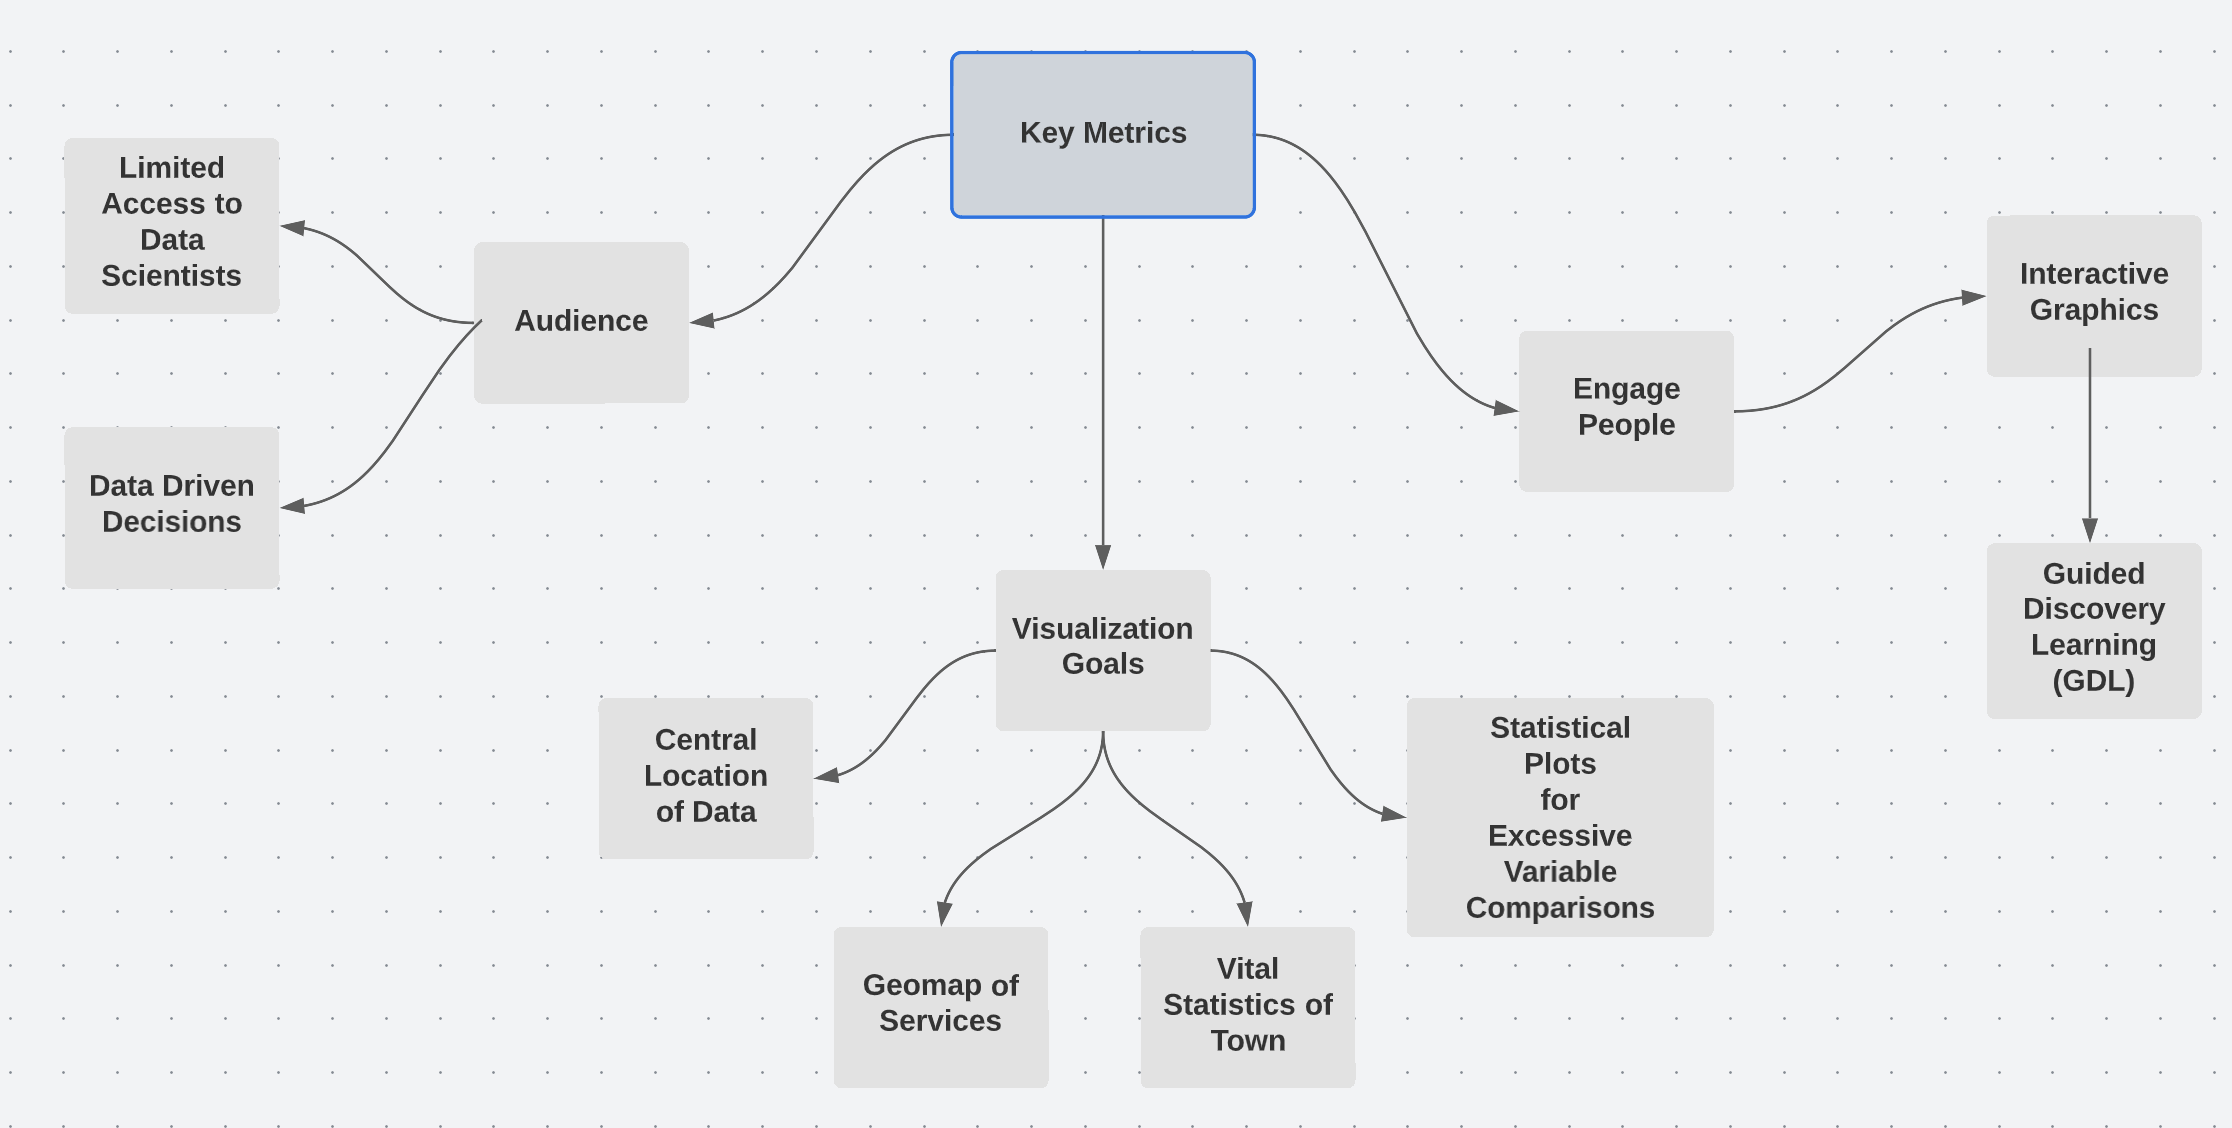
\includegraphics{figure/KeyMetrics.png}
\caption{Diagram of considerations for our dashboard design process.}\label{fig:metrics}
}
\end{figure}

One problem we identified early in the process of assessing smart-shrinkage strategies in small towns is that these towns do not have the resources to make data-driven decisions. Typically, small towns in Iowa are managed by at most a few part-time employees or volunteers. In some cases, essential management functions of the town are paid, but the municipalities we are interested in do not have sufficient funding to hire professionals to gather and analyze data.

As part of a wider project investigating the strategies towns use to maintain quality of life amid shrinking population, our research team provides communities with data about their own town, but also comparable towns across the state which may have a different approach to city services. In combination with other engagement strategies that are more qualitative, we hope to use this interactive dashboard approach to assist small Iowa cities with generalizing and developing strategies to improve or maintain quality of life amid shrinking populations.

One factor at the forefront of our visualization design is the importance of reducing the cognitive demands on viewers: we have assembled an incredible amount of data, and it is easy for even statisticians who deal with much larger datasets to get lost in the details of this data. At the same time, we want to invite viewers to engage with the data - to imagine, to draw comparisons, to generalize across towns, and to integrate outside information into the conclusions drawn based on the data we present.
This invitation to engage with the data is similar to the approach advocated in Guided Discovery Learning, a framework leverages hints, feedback, and other helpful information to guide users in interactive exploration (DeDonno, 2016).

We expect that users will be interested in ``sets'' of variables from the wider dataset, which we assembled based on quality of life factors in the Iowa Small Town Poll (David J. Peters, 2019). For instance, users might be interested in medical and social services available to residents, such as a local primary care clinic, nursing homes which are within driving distance, and the distance to the nearest emergency room; these factors might be explored separately from variables describing the services provided directly by city government, such as parks and recreation expenditures, snow removal services, and the distance to the closest fire station.

As a consequence of this massively multivariate structure, we very quickly focused on the use of parallel coordinate plots; other alternatives, such as tours (Wickham, Cook, Hofmann, \& Buja, 2011), require much more sustained attention to interactive plots as well as a deeper understanding of projections in multidimensional space which we cannot assume our users will have. Introduced in the 1880s (d'Ocagne, 1885), parallel coordinate or parallel set plots feature a series of vertical axes representing different variables arranged horizontally, with lines connecting each observation. When representing categorical data, parallel set plots may show ``blocks'' of data instead of individual lines, and are useful for representing conditional relationships between adjacent variables (Bendix, Kosara, \& Hauser, 2005); modifications of this design, such as common-angle plots (Hofmann \& Vendettuoli, 2013), address the issues which arise due to line-width illusions VanderPlas \& Hofmann (2015a). Parallel coordinate plots have been generalized to allow for continuous data and additional summaries beyond individual data points, such as densities (Heinrich \& Weiskopf, 2009). In this paper, we use the \texttt{ggpcp} package, which leverages the grammar-of-graphics framework introduced in Wickham (2016), allowing us to use not only parallel coordinate plots, but also to overlay other statistical summaries, such as boxplots or violin plots, to provide additional context about the marginal distributions of each variable in addition to allowing for exploration of the multivariate space.

We also anticipate that users will be interested in comparing their town to other, similar towns. We will discuss the different ways that this comparison strategy was implemented in each dashboard in the next section, which describes the evolution of the dashboard over time and accounting for feedback from users and other researchers on the wider project.

One final component of this project is that our dashboard is part of a wider effort to work with towns to understand the different strategies used to maintain resident quality of life amid shrinking populations. Thus, while the town leaders are our primary audience, we also are creating this applet for use in parallel with a team of other researchers: sociologists, economists, city planning specialists, and artists. These researchers opinions and feedback about the dashboard are also useful and important, as they regularly work with town leaders in different capacities and have an understanding of what factors are most important to them and what types of questions these leaders may have when faced with data and unfamiliar statistical visualizations.

Throughout the design process, we will assess our visualizations to determine which strategies for user interface and interactive graphics design are most useful to empower town leaders to make discoveries in publicly available data assembled with a focus on items that impact rural quality of life.

\hypertarget{guiding-design-principles}{%
\section{Guiding Design Principles}\label{guiding-design-principles}}

Research on dashboard creation and interactive visualization tends to be very task-specific and hard to apply to more generalized settings. That is, it is relatively easy to create a dashboard that works for a particular task, but it is hard to generalize from that process what will work for the next dashboard. With this in mind, we set out to clearly document our intentions at each stage of the design and evaluation process, with the goal of gathering some useful information about general dashboard design from the process of creating this specific dashboard.

Thus, our initial set of dashboard design principles is as follows:

\begin{itemize}
\item The town leaders are the focus audience; thus, the town itself should be the central focus of the app.
\item We should facilitate comparisons with other towns in order to allow the user to explore other potential solutions to offering services that enhance resident quality of life.
\item We will present the user with peer comparisons in order to widen the scope of exploration beyond the initial set of obvious peers in the local region.
\item We will implement feedback mechanisms that allow us to provide more detailed data and respond to feature requests to improve the dashboard design over time.
\end{itemize}

As with many dashboards, this project is under continuous development; while it makes for an unsatisfactory conclusion, we do not have a ``final'' dashboard design because the application will continue to evolve. However, we have some useful insights into the process of creating an application designed to invite users to explore a large and complex dataset that we believe to be a useful contribution to work in this area.

\hypertarget{dashboard-design-process}{%
\section{Dashboard Design Process}\label{dashboard-design-process}}

\hypertarget{dashboard-components}{%
\subsection{Dashboard Components}\label{dashboard-components}}

In this section, we discuss the philosophy behind the basic ``building blocks'' of the dashboard. This philosophy is present in all of the iterations of the dashboard that we present in this discussion, and we will evaluate the overall philosophy's effectiveness in the conclusion.

The large set of publicly available data (primarily from \url{data.iowa.gov}) we have assembled is useful, but we must be careful with how we present this data because it would be easy to overwhelm the user with small details that mask the bigger picture. We select a small subset of towns (out of the 999 towns in Iowa) and a small subset of variables of interest to start with, and then allow the user to increase the complexity of the display in accordance with their interest. This avoids some of the pitfalls of dashboard design that can easily lead to user overload (Few, 2006).

Our primary objective is to provide users with a town-centric approach: their town is at the center of our application, and comparisons to other, similar towns are secondary. As a result, the next component of the dashboard is intended to provide a brief overview of the information we have about a specific town of interest. This design is based on research into visualization sensemaking (Lee et al., 2016), in that we allow users to explore outward from the familiar to the unknown. The map visuals were built using Open Source Routing Machine (OSRM) route functions (Luxen \& Vetter, 2011) in R (R Core Team, 2022) to amplify the accuracy of the distances from necessary services in town-centric point. OSRM allows for finding the ``As the Crow Flies'' distance and time on the road for our vital services map, since OSRM technology is similar to Google maps.

When faced with the next component, a parallel coordinate plot (PCP), a novice user will be able to determine two basic components: Visual Object (textual objects and non-textual objects) and Frame (frame of content and frame of visual encoding).

Taken together, the app is a single page; the initial ``solid ground'' which the user explores from consists of maps showing the route from the center of town to necessary services, including the fire department, schools, post offices, and hospitals. In version 2, as shown in \autoref{fig:v2}, the map portion is condensed, and more space is given to value boxes that show vital statistics about the town's QoL and financial metrics. This relatively straightforward display is followed by a parallel coordinate plot that allows the user to see similar towns along dimensions such as economic indicators or population size.

\hypertarget{initial-draft}{%
\subsection{Initial Draft}\label{initial-draft}}

The initial design sketch and implementation are shown in \autoref{fig:v1}.

Users' towns are at the center of our application, and comparisons to other, similar towns are secondary. As it can be extremely difficult to predict which towns are optimal for comparison purposes (similar may involve population, region, economic indicators, sports rivalries, and any number of other variables), we allow users to modify a set of suggested comparison towns to indicate other towns of interest.

\begin{figure}
\centering
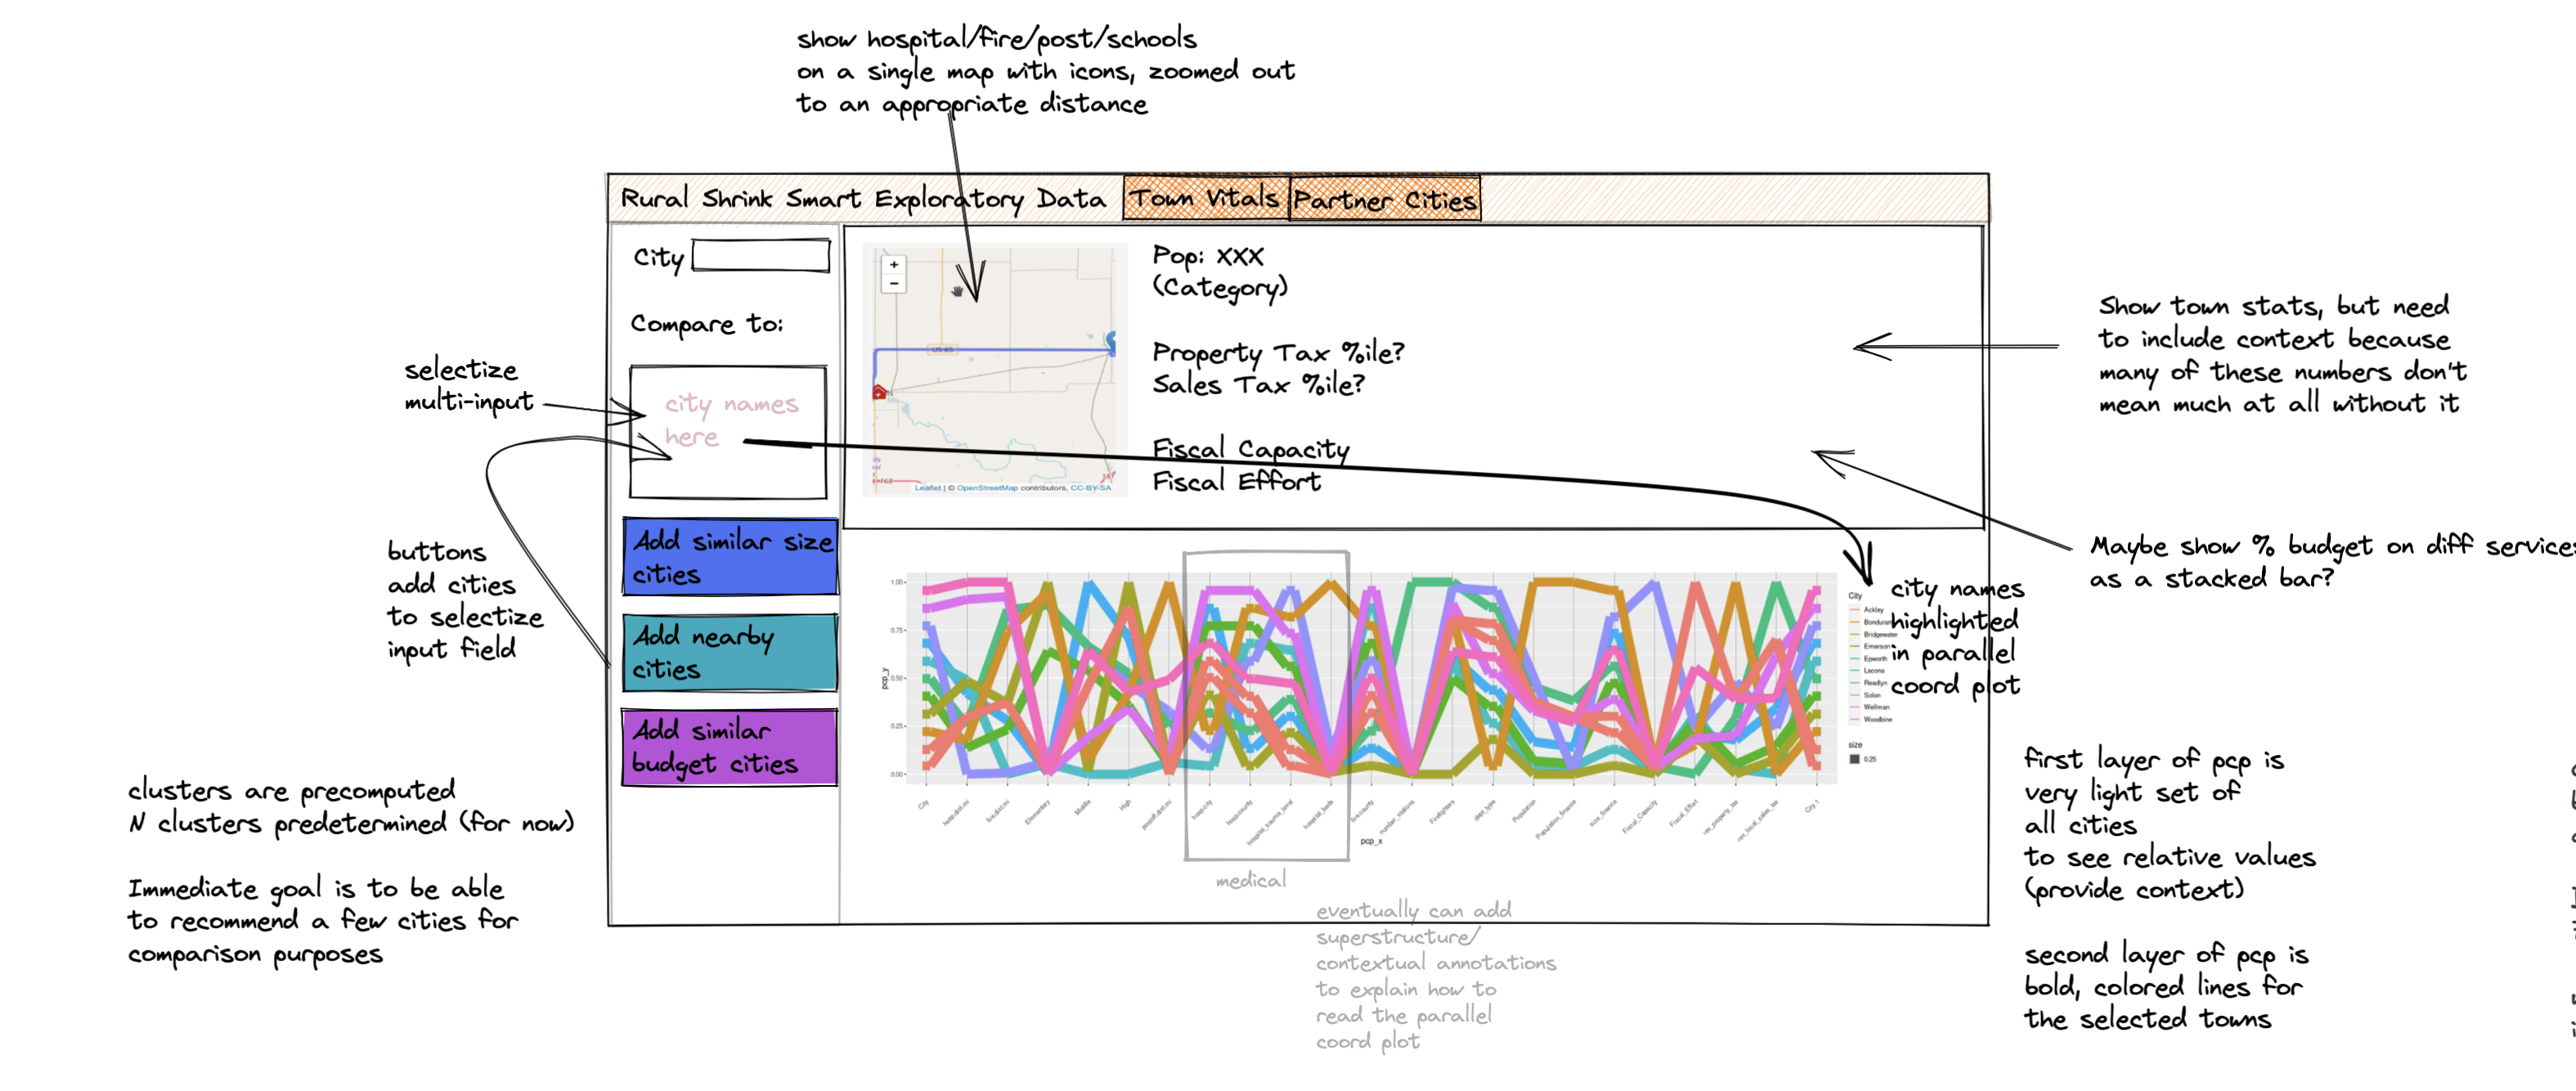
\includegraphics[width=\textwidth]{figure/Version1.png}

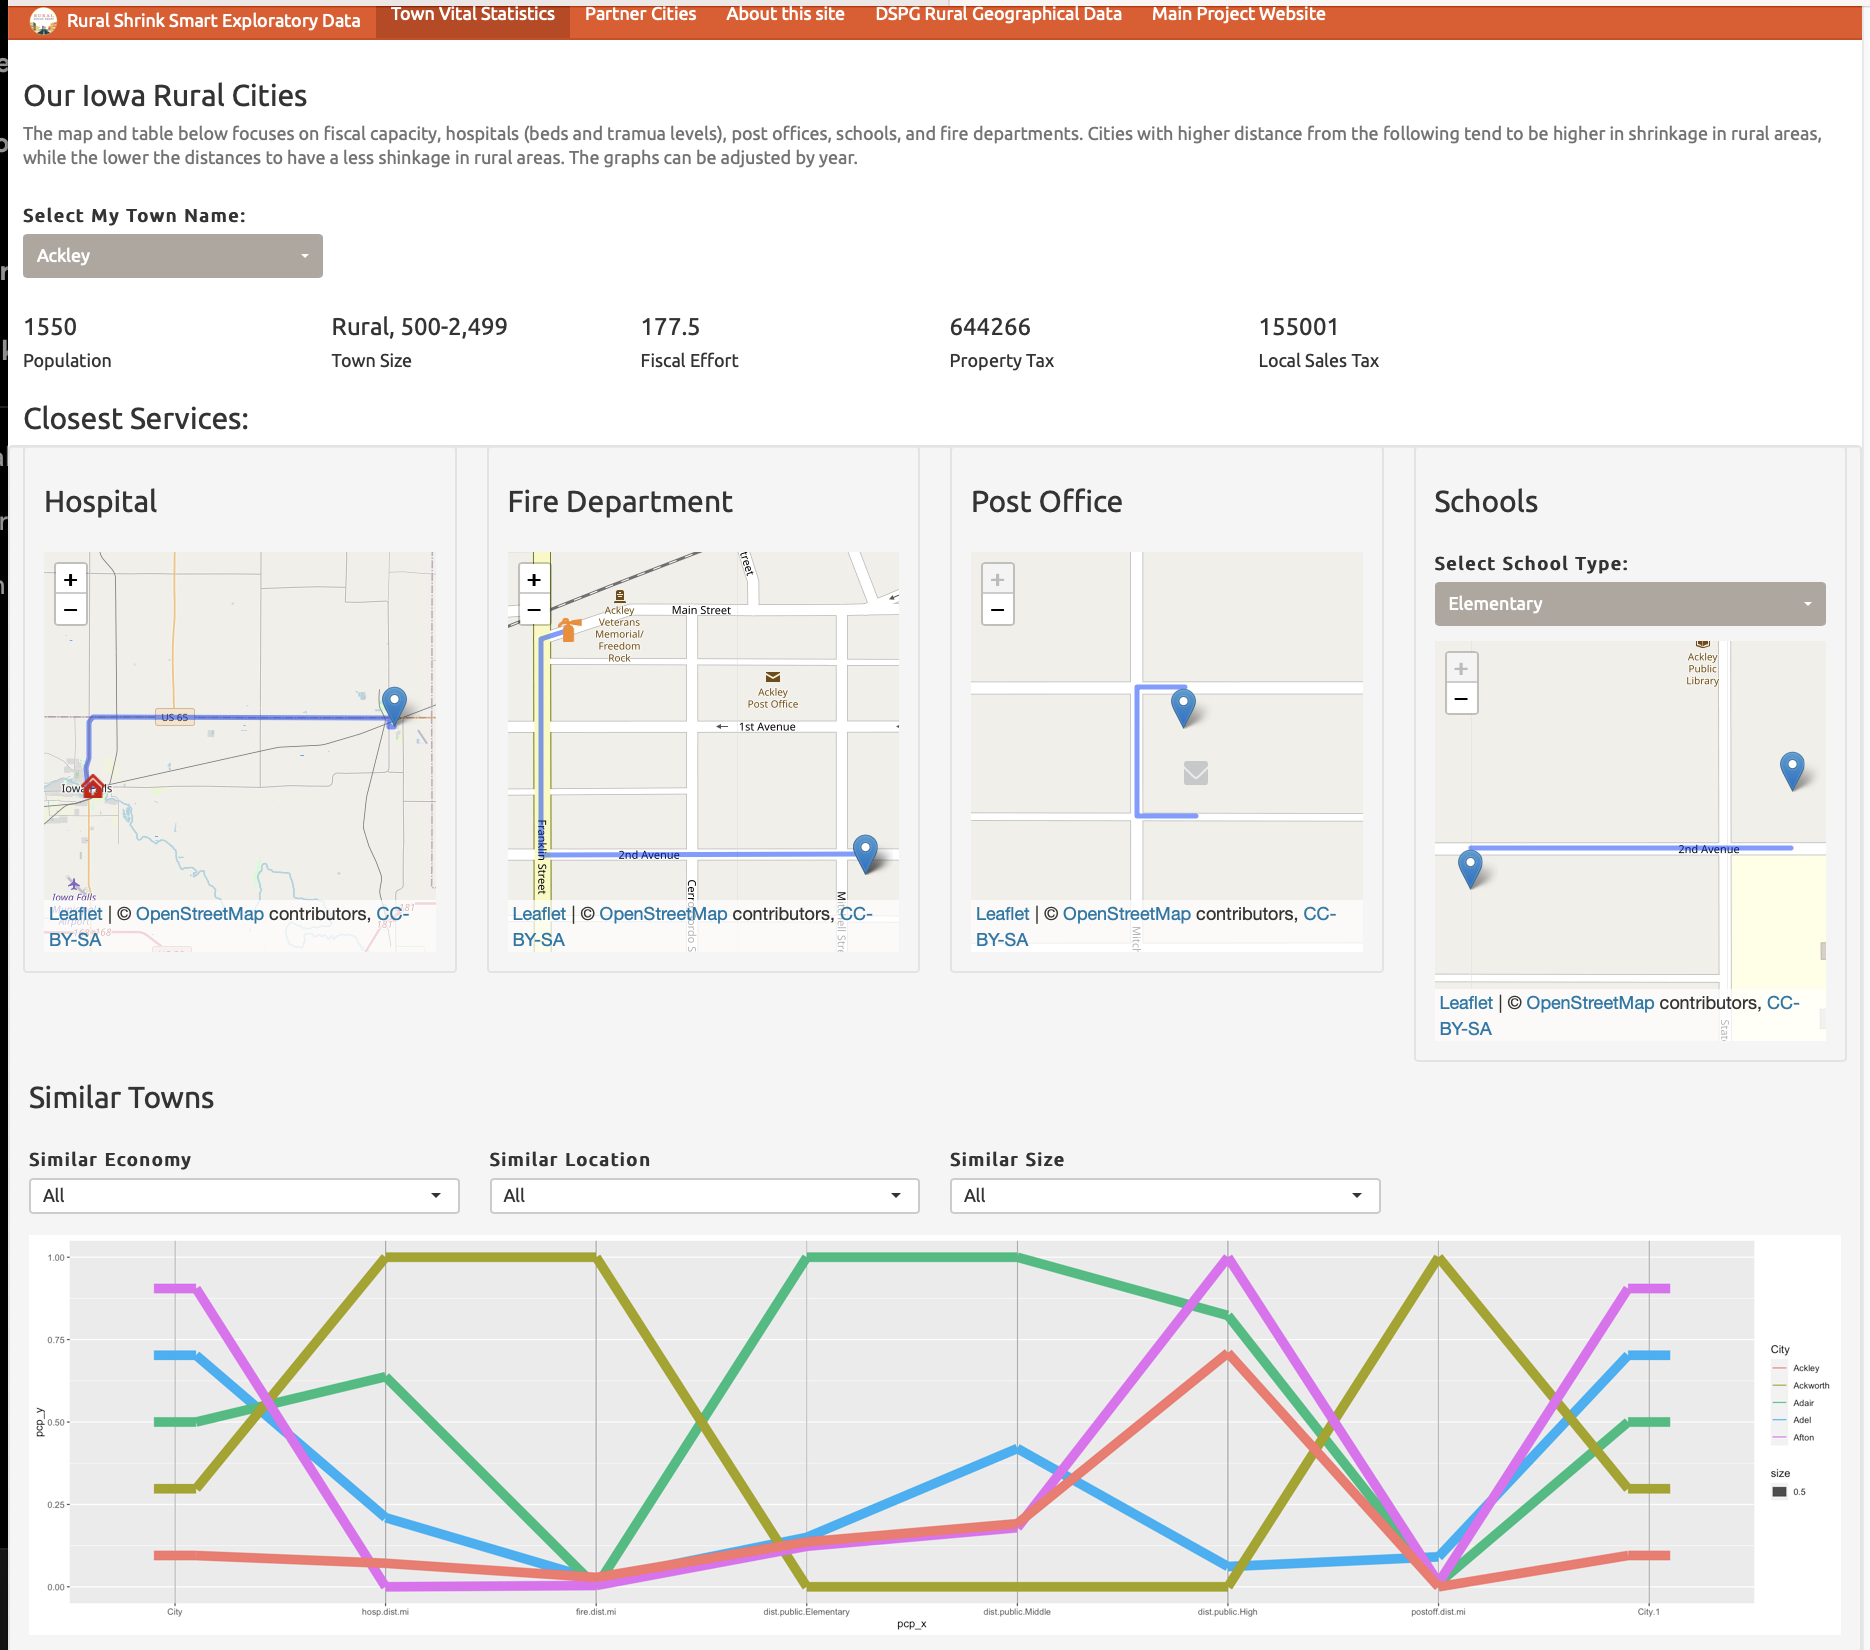
\includegraphics[width=.7\textwidth]{figure/Version2.png}
\caption{Initial dashboard design sketch (top) and implementation (bottom).}\label{fig:v1}
\end{figure}

We implemented some suggested town comparisons using unsupervised clustering methods to help our towns make decisions that are informed in comparison to similar towns, for budget size, population size and location. We initially focused on determining the next five to ten similar towns, based on distances to services. This feature became an important diagnostic for our data quality, as it became clear that towns which were grouped with big cities but which did not have a large population were so grouped because of missing data. Unfortunately, this clustering feature was not as useful to the application users, as they came to the dashboard with a pre-existing set of towns to compare to; our suggested comparisons were in the way.

The initial dashboard design featured several responsive maps showing the distance to the nearest hospital, fire department, post office, and school. These maps were ineffective for several reasons:

\begin{itemize}
\tightlist
\item
  Town residents already know this information (though it was useful for us as the dashboard designers, because we aren't nearly as familiar with the 900+ small towns in Iowa)
\item
  We computed distance from services relative to the center of town - coordinates provided in the data from \url{data.iowa.gov}. Generally speaking, the post office is at the center of town and the fire department is usually very close to the center of town; these two maps were useless. The school and hospital maps were less useless, but still did not provide particularly useful information to people already familiar with the town.
\item
  It became clear that it might be more useful to show the comparison towns on a map (relative to the town of interest) so that users could compare geographical ratings for unfamiliar data to familiar data.
\end{itemize}

In addition, we received feedback on the parallel coordinate plot at the bottom of the app which was surprising: the viewers (in this case, other researchers on the team) were not as intimidated by the parallel coordinate plot as we had expected. They did need some explanation of how to read the plot, and these hints need to be included in the dashboard, but they grasped the fundamental idea of the plot very quickly.

Our conclusion, based on this initial dashboard draft, was that we needed to restructure the application. Our attempt to show familiar information first to ``build up'' to the more unfamiliar structure of a parallel coordinate plot was not effective; there was too much clutter and not enough new information to draw users in.

\hypertarget{redesign}{%
\subsection{Redesign}\label{redesign}}

\begin{figure}
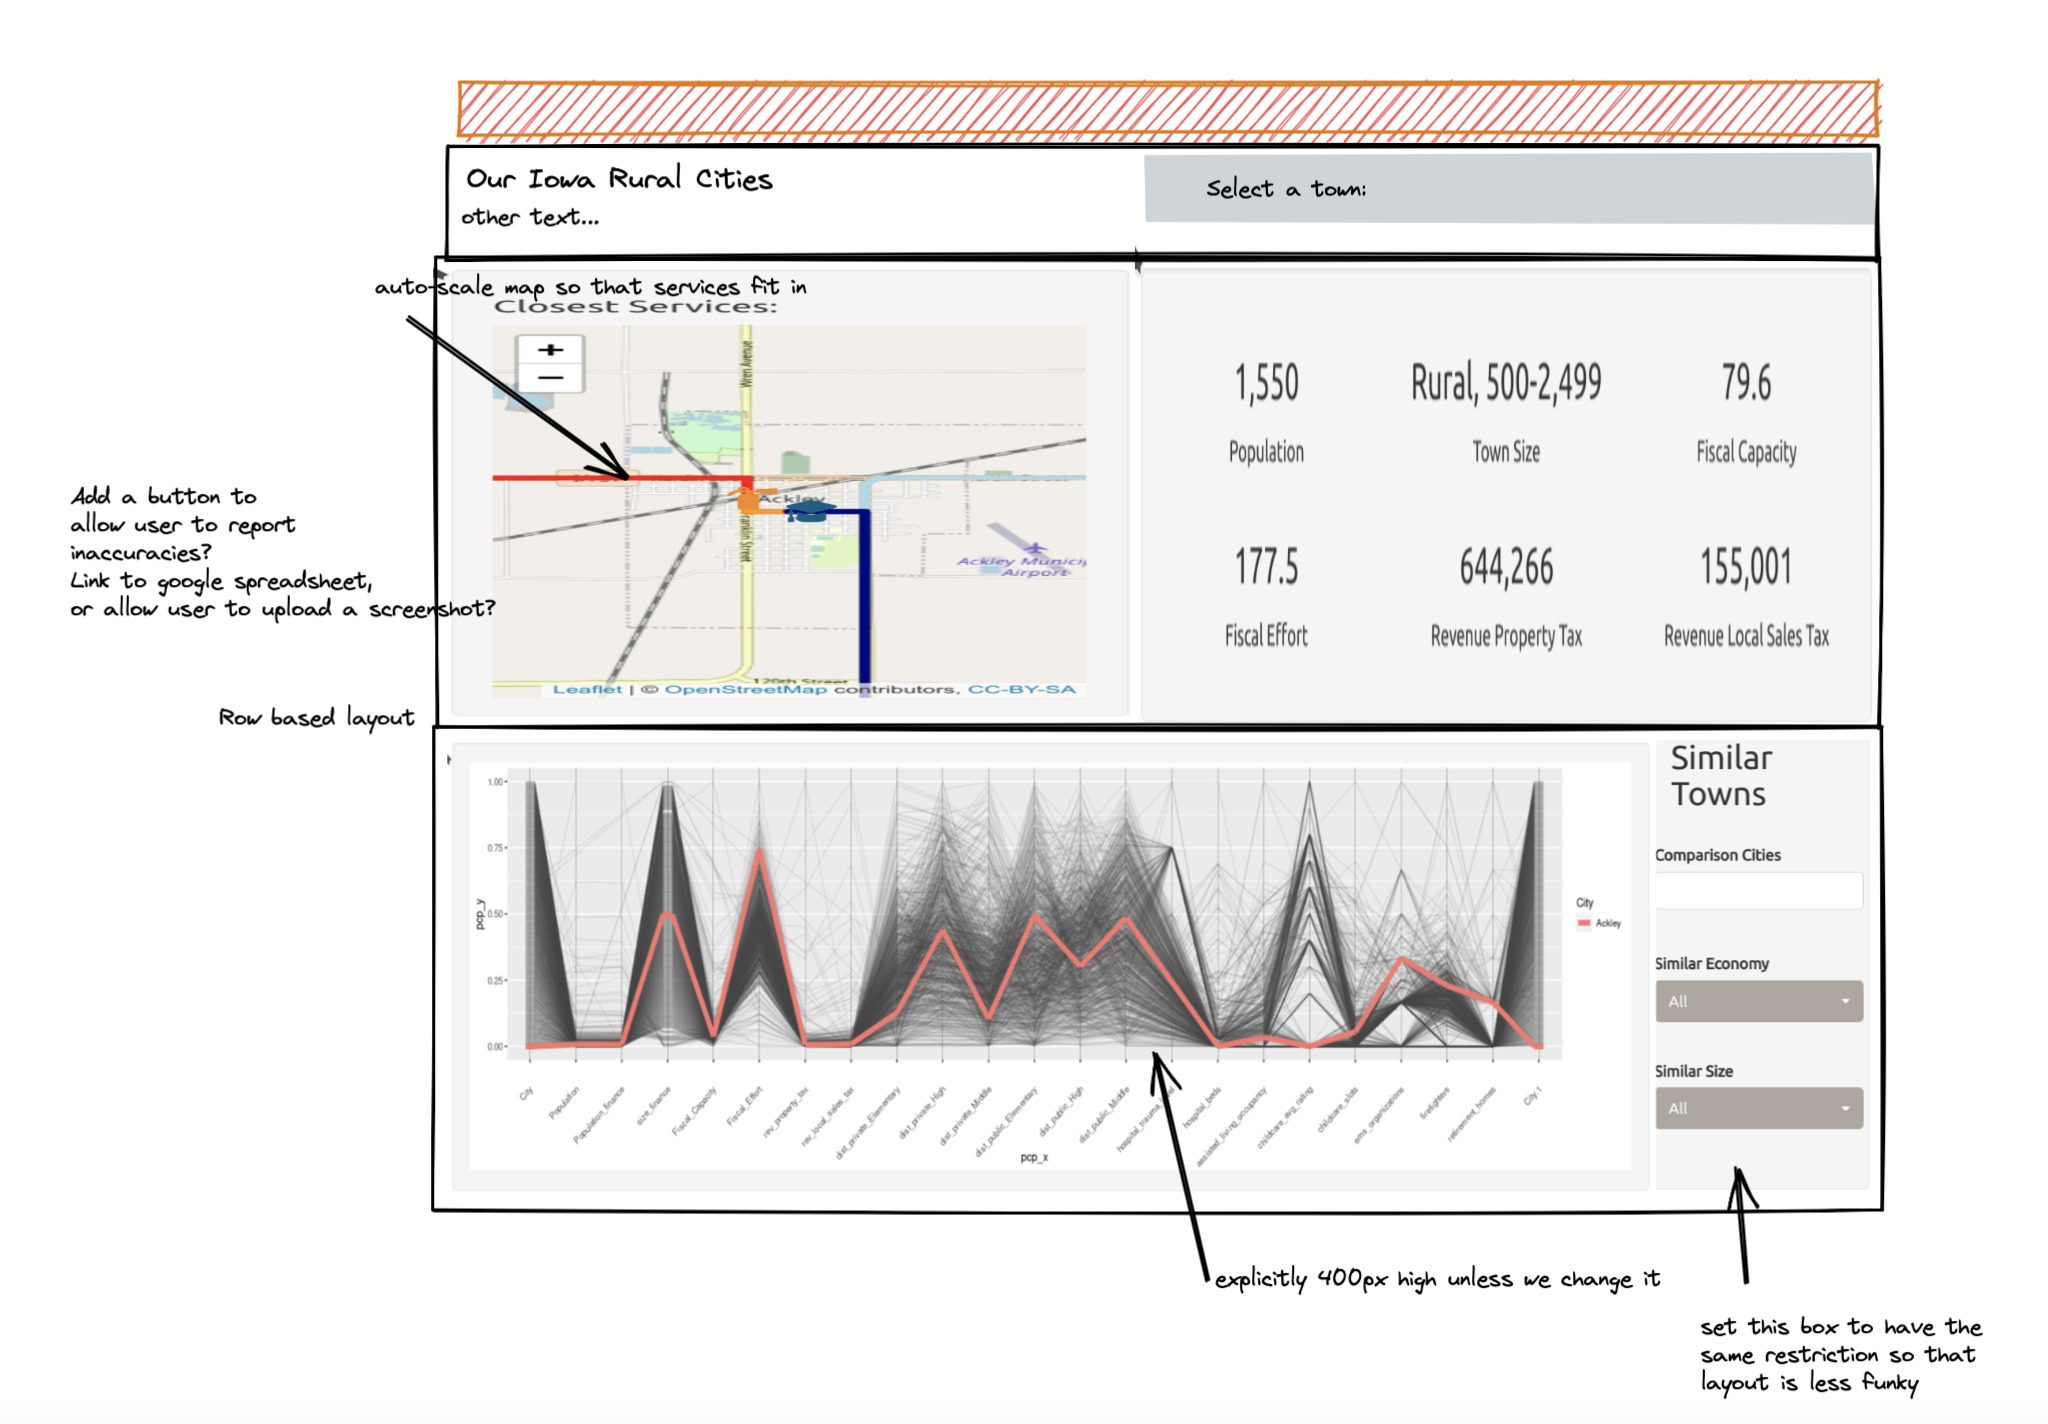
\includegraphics[width=.8\textwidth]{figure/Version3.png}

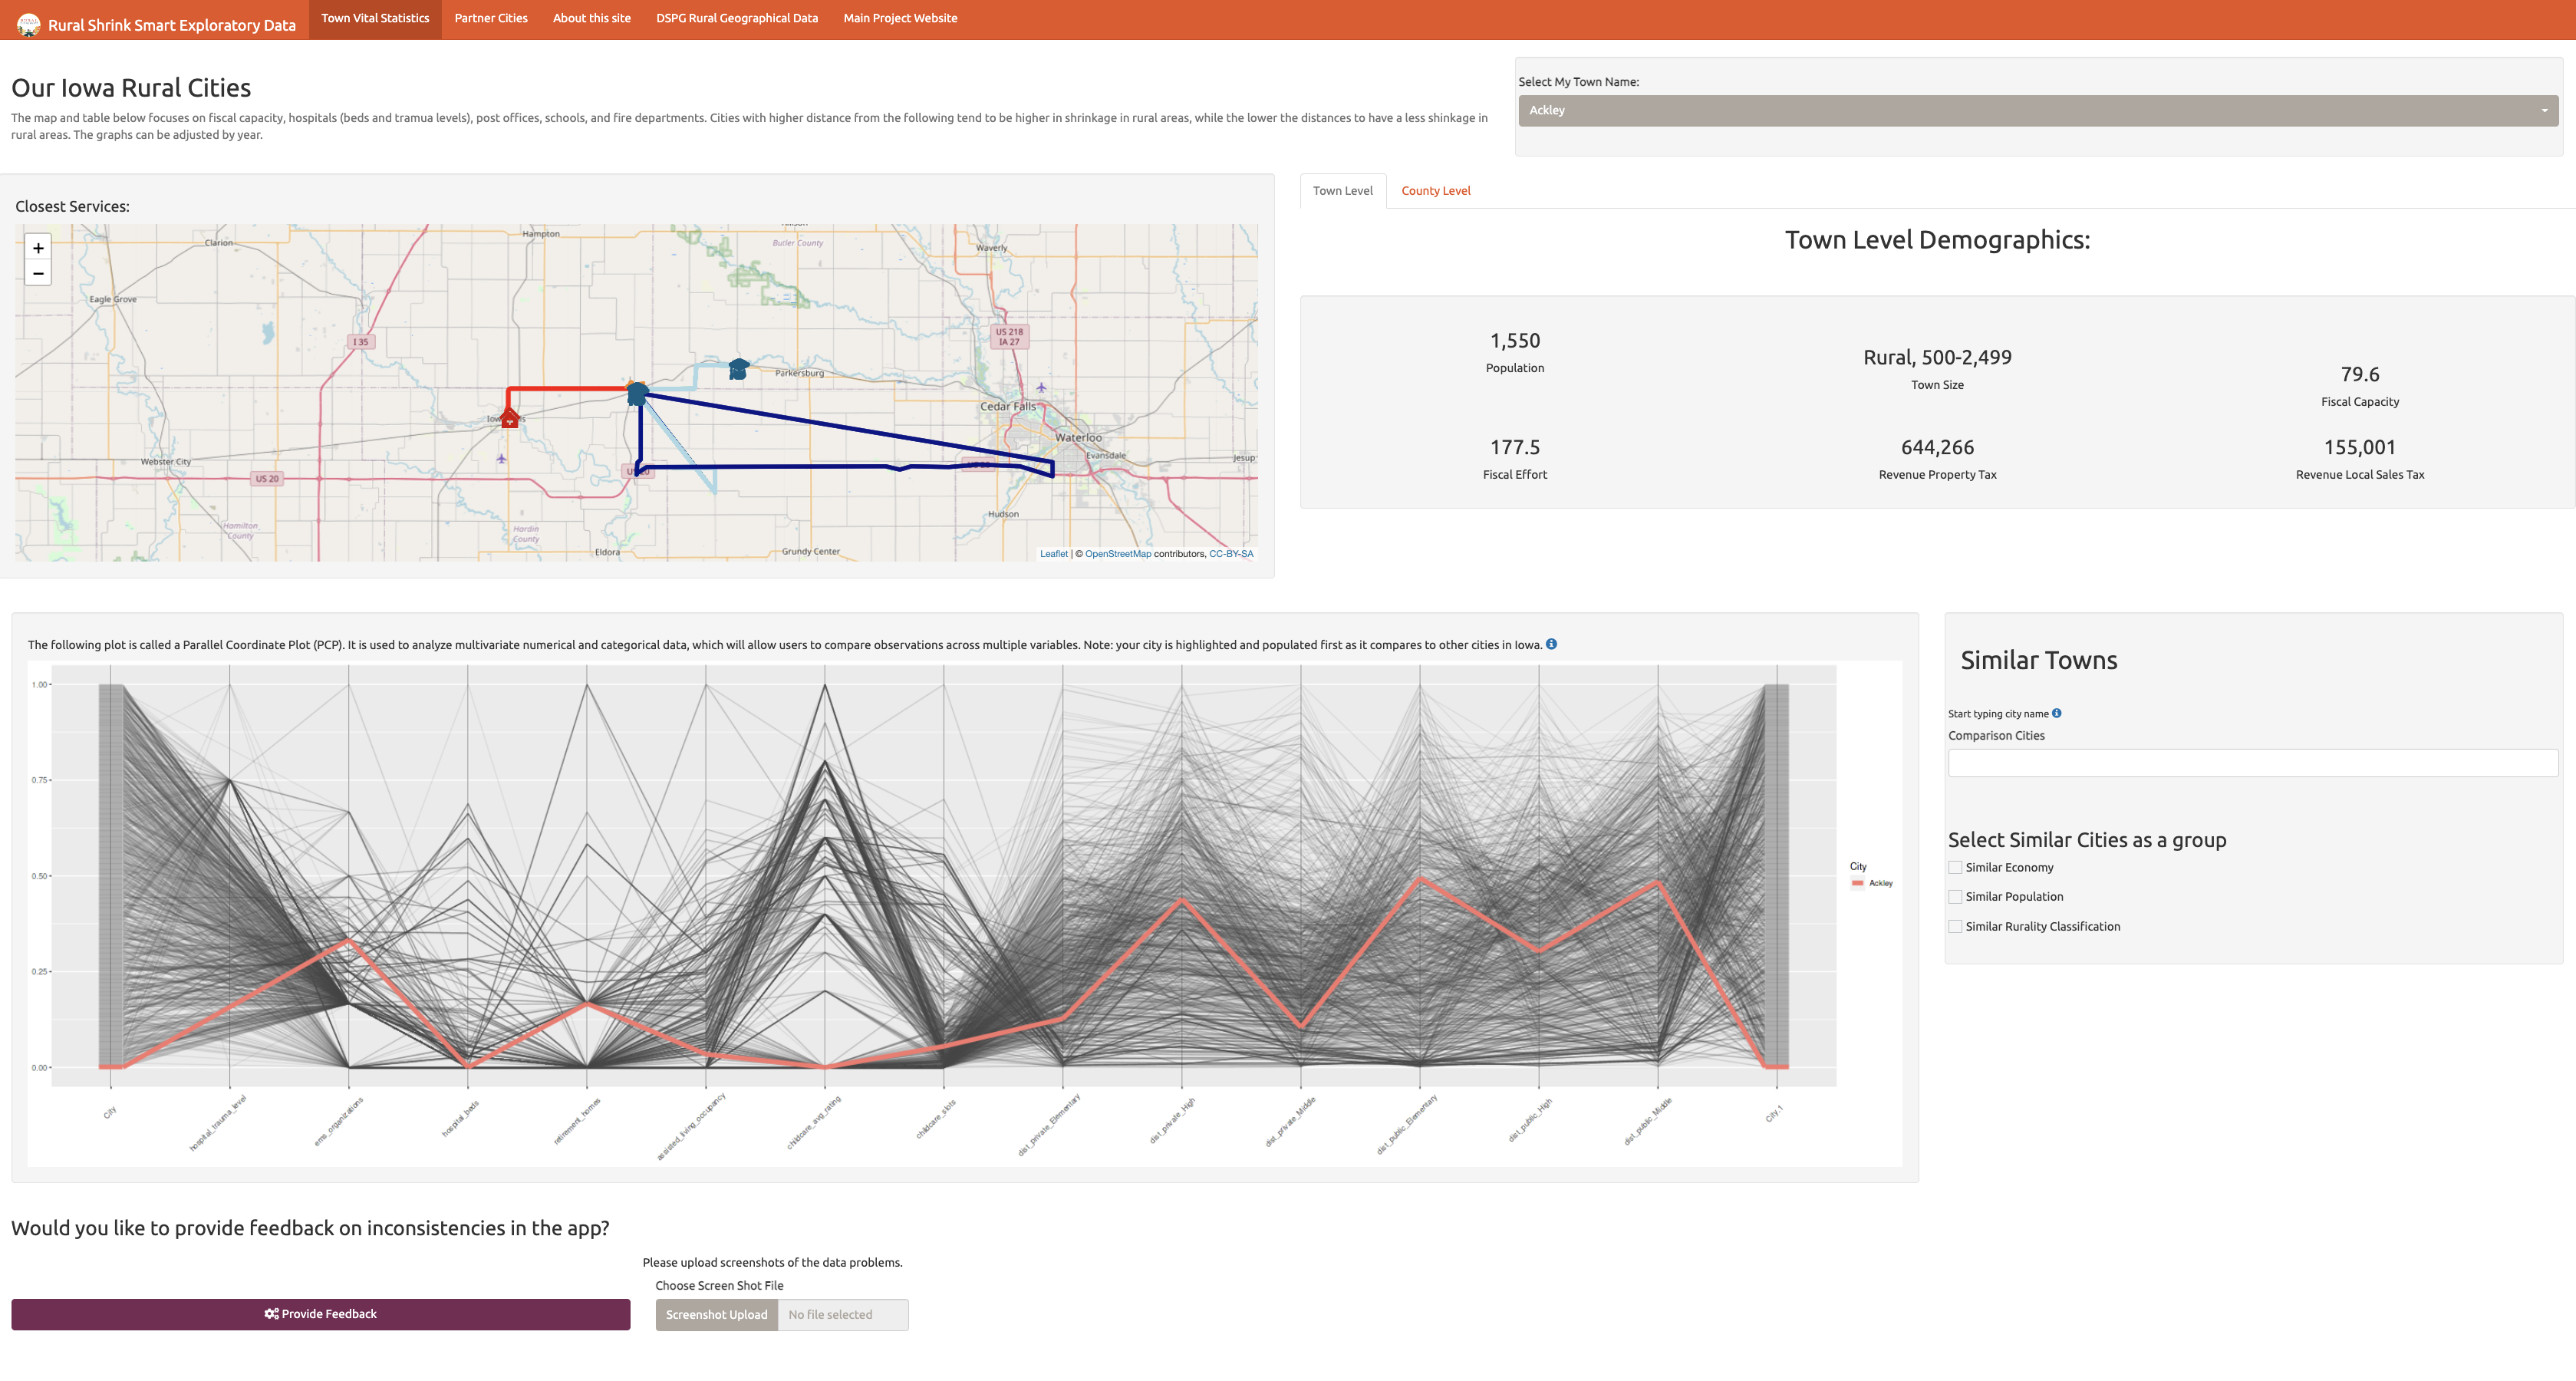
\includegraphics[width=\textwidth]{figure/Version4.png}
\caption{A second iteration of the sketched design (top) and the implementation (bottom).}\label{fig:v2}
\end{figure}

In the initial design, we included a map for each vital service, this initially created a lag for the users' experience. As a result, we cached map directions from OSRM for each service in our database, which drastically reduced the response time for the user. Our initial design did not naturally focus the user's eye on the most important parts of the dashboard; the redesign allowed for a cleaner flow from the top to the bottom.

In addition to the timing due to the map loading slowly, we added the vital statistics at the county level to allow for a more robust understanding of the town and it's surroundings. The rurality index provided a better classification and the USDA sources allowed for the town to understand the impact of the closest major city due to commuting for work and shopping at larger stores not available within the town.

We also modified the parallel coordinate plots in several ways:

\begin{itemize}
\tightlist
\item
  Our x-axis had a large number of variables that we as researchers believed to be the most strongly associated with quality of life. However, there were still too many variables for users to successfully parse. We reduced the number of variables, focusing on variables that had the highest data quality, and we grouped these variables by quality of life factor (David J. Peters, 2019).
\item
  Originally, parallel coordinate bands were scaled based on the selected comparison towns. This had the effect of truncating the range of variables and over-emphasizing differences between selected towns relative to the overall range of each variable over all towns in our data set. We chose to show all towns in the data set in a very light \(\alpha\) grey color to provide some information about the overall range of each variable. Unfortunately, even with the low-\(\alpha\) value, this increased the visual complexity of the plot and confused users. Future iterations will likely make use of another aesthetic, such as boxplots or violin plots, to show the range of values for all towns, and then use lines only for towns that are selected by the user. This should strike a balance between visual complexity and representing the data accurately.
\item
  We noticed that users did not make use of our suggested comparison towns, and so we removed that option in favor of allowing users to enter their own comparison towns directly. Users already had pre-determined towns they wanted to compare to, and our suggestions were just in the way.
\end{itemize}

While not all of these modifications were well received in our second round of user testing, the changes did incrementally move the dashboard display towards our goal of allowing users to explore the data and engage with it. We continued to be surprised with how well users reacted to the parallel coordinate plots, which we initially thought might be too abstract for users unfamiliar with multivariate data displays, but the ability to compare towns across multiple dimensions and examine the similarities and differences between their approaches to different services seemed to be intuitive for users once they understood that each vertical axis was a different variable.

\hypertarget{discussion}{%
\section{Discussion}\label{discussion}}

Our dashboard design philosophy worked primarily to promote a town-centric approach application with comparisons to other similar towns being secondary. This approach created a way for the user to see their town information at the top of the page and to explore the PCP after reviewing their own town's essential statistics. The PCP in the lower part of the dashboard allowed for the user to see the plot and adjust to the fact that they could add more towns to the plot, providing an opportunity to explore the wider dataset from a base of familiar knowledge.

While we initially framed the design around guided discovery learning, the approach did not seem to suffice for our user base; instead, we found that users were more drawn to the unfamiliar from the start. We will likely leverage this in future iterations by using visual forms such as flower plots to draw the users in; even though these plots are not ideal for numerical display of data, the visual novelty and aesthetic appeal will provide some motivation to continue exploring and thinking about the data.

One factor that we have briefly considered and have seen hints of in our user feedback is that towns may not want to be compared negatively with other towns. While users have very definite ideas about which towns they would like to compare to, we can always mask the town names and move back to comparisons based on town size and other factors (for instance, whether or not a town is the county seat is a factor that is important outside of population). Using this approach, we would label each town as ``Town 1'', ``Town 2'', and so on, which would eliminate some of the fears about negative comparisons, but would also remove some of the novelty of the data dashboard for our users and would prevent users from drawing on their own outside knowledge about each of the comparison towns.

We also recognize that we need to leverage the expertise of others in our research team: we are working with artists, researchers in architecture, economists, and sociologists; these researchers provide outside knowledge that we do not have and may be able to help us create insightful use-cases to showcase the app and teach towns how to use it. We can also leverage the app to connect users with our research team, providing additional value to those who use the applet and facilitating development of strategies for maintaining quality of life amid shrinking populations.

\hypertarget{future-work}{%
\section{Future Work}\label{future-work}}

One avenue we will explore in future iterations of the dashboard is to incorporate other dashboards generated by different groups within this project. This will create a wider field of information to explore: for instance, some of the additional work will focus on the 99 towns featured in the Iowa Small Town Poll; this will allow us to showcase survey-based measures of quality of life alongside the more objective measurements assembled in the dataset discussed in this paper. While at least one tab of this omni-dashboard will still focus on wider EDA and discovery, we hope to incorporate other information as well to provide a more well-rounded data display encompassing most of the facets of this complex project.

We are also mindful of a distinction between ``eye candy'' and purpose-driven data visualization. While we have typically focused on the latter, there is certainly a place in our dashboard for the former as well. ``Eye candy'' visualization is intended to draw the viewer in and motivate them to explore; while these visualizations may not be particularly effective at communicating quantitative information, if they motivate the user to engage with the rest of the dashboard, they still serve a purpose. It is with this mindset that we intend to explore the use of flower plots - the artistic opportunities combined with the display of quantitative information (even in a form that isn't optimal for quantitative comparisons) may be useful to engage viewers before transitioning to more useful data visualizations intended to provide accurate quantitative comparisons.

EDA can be a difficult for a variety of groups of people, novice users and experienced researchers. One of the more difficult components of this project has been clearly articulating the purposes of EDA to a diverse group of researchers unfamiliar with the concept. One of the most useful parts of this dashboard iteration process has been as an aid to data discovery: that is, the dashboard motivated us to find additional data sources and incorporate them into the project. Having conversations with other researchers about the EDA process helped to facilitate these conversations, as each discussion seemed to uncover additional data sources that someone remembered after looking at the dashboard. While this facet of the dashboard process may be difficult to study formally, it would be an interesting avenue for investigation.

\hypertarget{conclusions}{%
\section{Conclusions}\label{conclusions}}

In this paper, we have documented the process of designing a dashboard for exploration and visualization of a large and complex data set assembled from many different sources. Our primary audience was leaders of small towns in Iowa, with a secondary audience of researchers in fields other than statistics collaborating on this project with us. Through the process of revising our dashboard, we found that the idea of guided discovery learning as implemented in our first version did not work as well as we had anticipated. It was more important to focus on allowing users to explore their questions about the dataset by facilitating user-driven comparisons and exploration, rather than attempting to anticipate user desires by providing comparison towns. In addition, we found that it would be more effective to draw users in with novel visual displays, as these seemed to attract more interest than providing known facts and an opportunity to explore outwards from an initial area of familiarity.

While it is hard to apply the findings from one fairly specific visualization project more widely, there is a lack of resources in this area that provide both design philosophies and actual analysis of user feedback in a qualitative sense. We have attempted to address this dearth of information by providing the design strategies, user feedback, and our planned and executed modifications, in the hopes that others facing the daunting challenge of designing a dashboard for EDA may learn something from our experiences.

\hypertarget{math-sci}{%
\chapter{Chapter 2 Stuff}\label{math-sci}}

\hypertarget{chapter-paper-on-rural-shrink-smart-manuscriptsubmitted-to-journal-of-data-science-special-issue}{%
\chapter{Chapter Paper on Rural Shrink Smart Manuscriptsubmitted to Journal of Data Science Special Issue}\label{chapter-paper-on-rural-shrink-smart-manuscriptsubmitted-to-journal-of-data-science-special-issue}}

\hypertarget{introduction-2}{%
\section{Introduction}\label{introduction-2}}

As the amount of data has increased in nearly every facet of life, the need to make sense of that data in an approachable, accessible form has become ever more important.
As a result, many companies and organizations use interactive dashboards to present these data in a more useful and visually appealing form (Sarikaya et al., 2019).
In many cases, dashboards support viewers' information processing, helping to make sense of complex data, navigate through a dataset, and supporting decision making based on the data.

Dashboards are often used, as with the car display of the same name, to provide summary information about many separate attributes of a common entity. One glance at a car's dashboard will tell you the speed, RPM, engine temperature, amount of gas in the tank; more importantly, however, the goal is not for the user to remember all of these characteristics, but to assess whether any of these quantities is outside of the expected range.
Similarly, interactive dashboards for data are often used to display many different attributes and performance metrics which are of importance for stakeholders.

In this paper, we discuss the process of designing a dashboard to present publicly available government data to stakeholders in small Iowa towns to facilitate decision making and objective comparison with other similarly-situated towns.

Some communities continue to thrive as they lose population because they adapt, maintaining quality of life and community services for residents while investing in the future. This process, \emph{smart shrinkage}, is important for rural areas who have experienced shrinking populations for decades. As small rural towns, defined in the Iowa Small Town Poll as towns with between 500 and 10,000 people in the 1990 census (David J. Peters, Hamideh, Zarecor, \& Ghandour, 2018), do not have access to data scientists or even the ability to easily leverage data collected locally to support decisions, our research team will provide communities with data about services in small town Iowa in order to assist with developing strategies to improve quality of life for their residents amid shrinking populations (Rural Shrink Smart Team, 2022). We hope to allow towns to explore their own data and compare to other similar towns, centering decision-making on data in the context of small-town Iowa life.

\section{Data Description}

The Smart and Connected Community (SCC) dashboard data are primarily assembled from \url{data.iowa.gov} (State of Iowa, 2020), with some additional datasets assembled from federal and private sources. Most of these data sets are collected at a town/city or county spatial resolution, requiring us to carefully join data to ensure that these differences are respected while collating relevant information at the city level. In addition to the more commonly available statistics derived from e.g.~the census and American Community Survey, \url{data.iowa.gov} contains several unique data sets, including local liquor sales, school building locations, town budgets and expenditures, hospital beds, Medicaid reimbursements, and other details that may provide information about local quality of life.

Data available on Iowa's data portal were augmented in some cases with higher-quality data sets in cases where the Iowa data were out of date or insufficiently accurate.
Data collected from ELSI (National Center for Education Statistics, 2020) from \url{https://nces.ed.gov} were used to show the distance to any private or public school. The National Center for Education Statistics (NCES) is the primary federal entity for collecting and analyzing data related to education (Zarecor et al., 2021).

Data collected from the Index of Relative Rurality (IRR) (USDA - ERS, 2020a) were used in the SCC dashboard to help classify the towns. The IRR is a continuous, threshold-free, and unit-free measure of rurality. It is an alternative to the traditional discrete threshold-based classifications.The IRR ranges between 0 (low level of rurality, i.e., urban) and 1 (most rural). Four steps are involved in its design:

\begin{enumerate}
\item Identifying the dimensions of rurality: population size, density, remoteness, and built-up area.
\item Selecting measurable variables to adequately represent each dimension:
    \begin{itemize}
        \item Size: logarithm of population size
        \item Density: logarithm of population density.
        \item Remoteness: network distance.
        \item Built-up area: urban area (as defined by the US Census Bureau) as a percentage of total land area.
    \end{itemize}
\item Re-scaling the variables onto bounded scales that range from 0 to 1.
\item Selecting a link function: unweighted average of the four re-scaled variable.
\end{enumerate}

Data collected from Rural Urban Commuting Area Codes (USDA - ERS, 2020b) were used to help identify towns with commuting behaviors in our rural areas. The rural-urban commuting area (RUCA) codes classify U.S. census tracts using measures of population density, urbanization, and daily commuting. This data is on a zip code-level that will help identify those communities that commute to more urban areas. The most recent RUCA codes are based on data from the 2010 decennial census and the 2006-10 American Community Survey. The classification contains two levels. Whole numbers (1-10) delineate metropolitan, micropolitan, small town, and rural commuting areas based on the size and direction of the primary (largest) commuting flows.

One of the interesting features of this assembled data set is that missing data can be missing for multiple reasons: not all state data is complete, but data about certain services may also be missing because towns do not offer that service.
Thus, in addition to the usual challenges of working with real-world data that is ``messy'' in a variety of ways, we also have to contend with missing data that is missing due to the size of the community or the lack of services. This makes both visualization and statistical analysis more complicated (and more interesting).

\hypertarget{dashboard-design-considerations-1}{%
\section{Dashboard Design Considerations}\label{dashboard-design-considerations-1}}

\begin{figure}
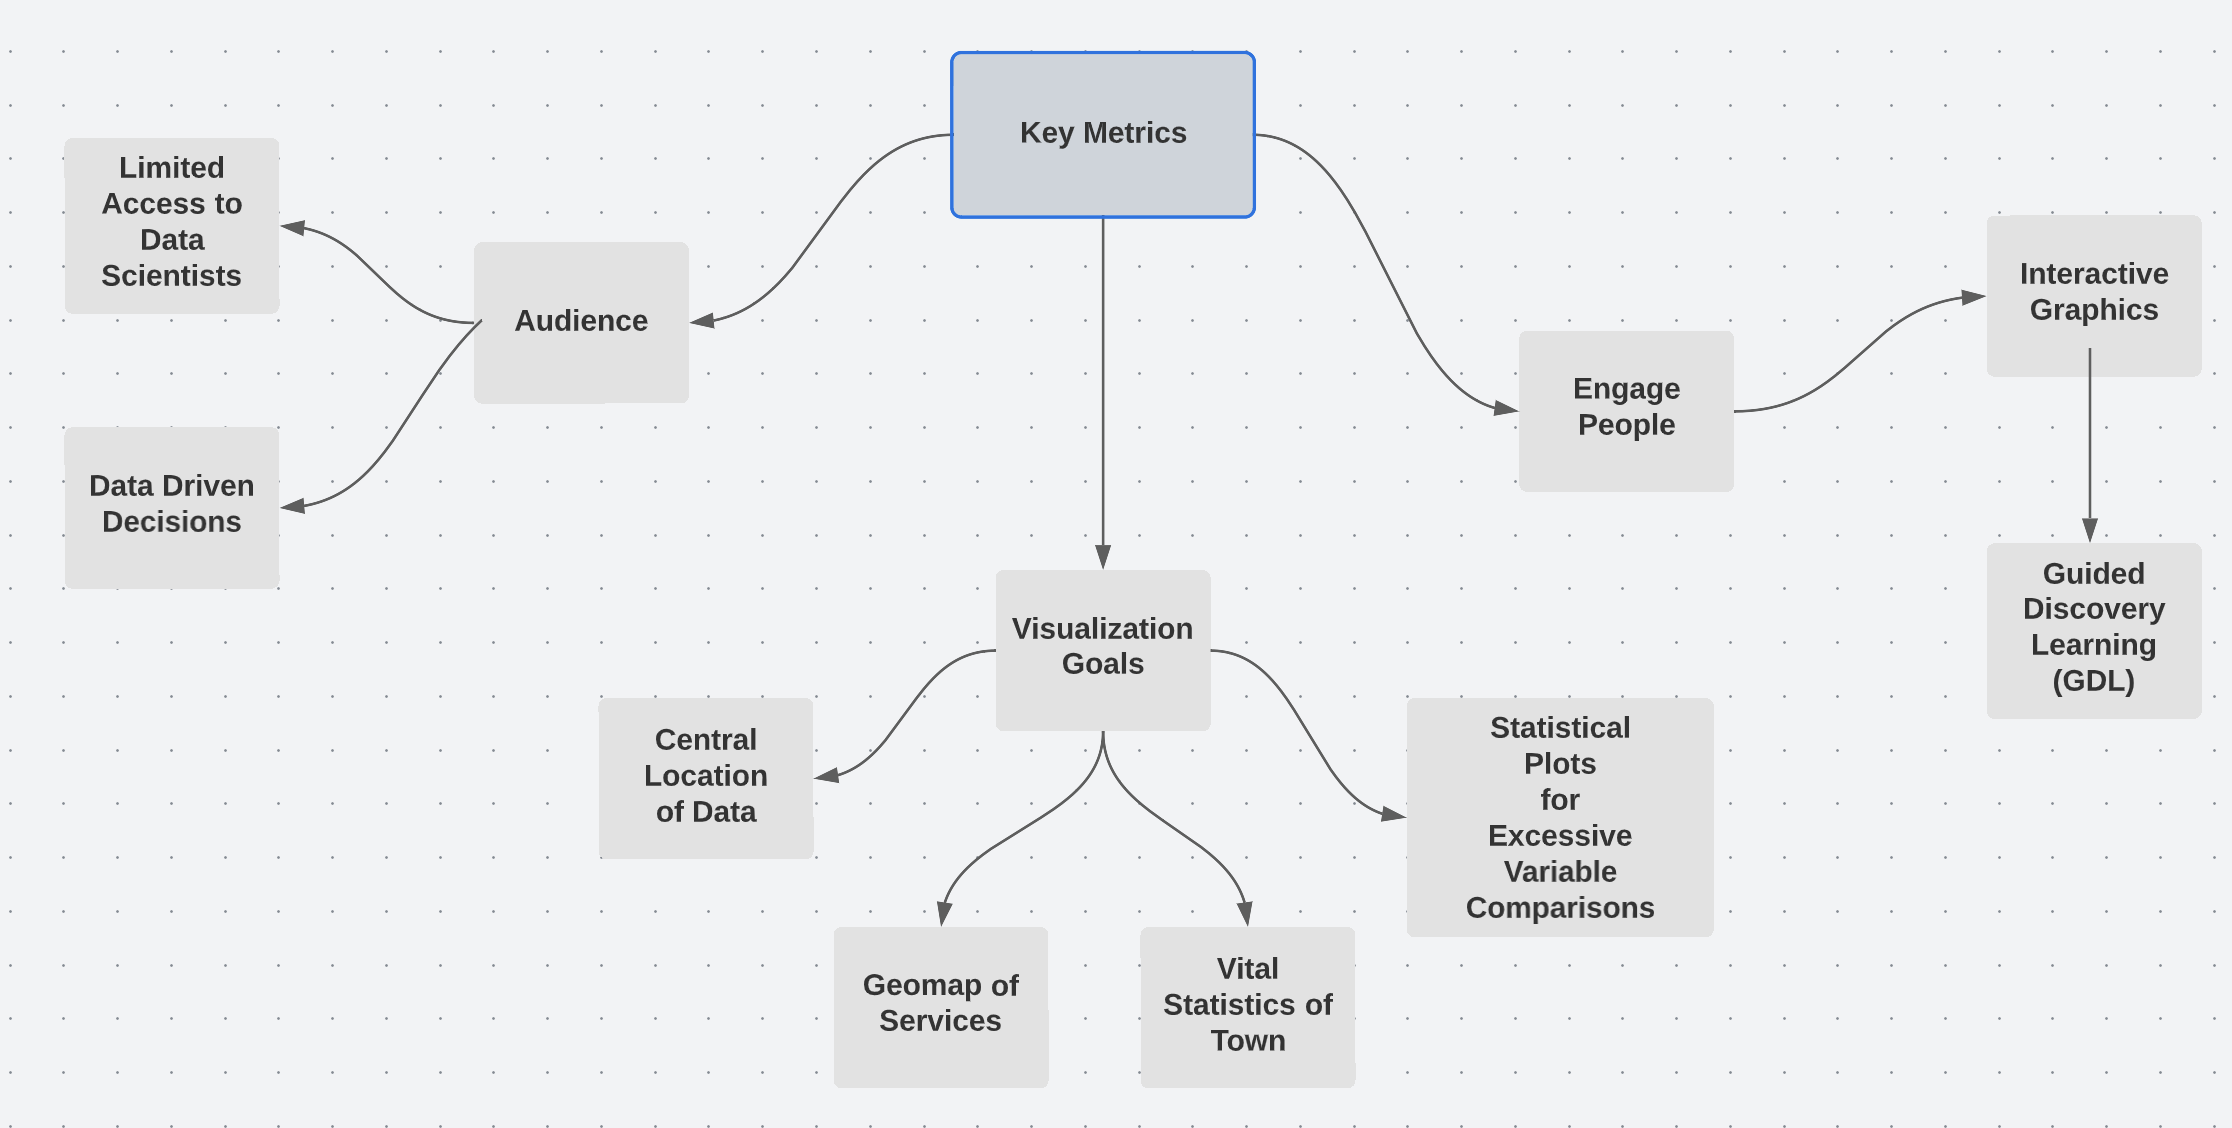
\includegraphics[width=.8\textwidth]{figure/KeyMetrics.png}
\caption{Diagram of considerations for our dashboard design process.}\label{fig:metrics}
\end{figure}

One problem we identified early in the process of assessing smart-shrinkage strategies in small towns is that these towns do not have the resources to make data-driven decisions. Typically, small towns in Iowa are managed by at most a few part-time employees or volunteers. In some cases, essential management functions of the town are paid, but the municipalities we are interested in do not have sufficient funding to hire professionals to gather and analyze data.

As part of a wider project investigating the strategies towns use to maintain quality of life amid shrinking population, our research team provides communities with data about their own town, but also comparable towns across the state which may have a different approach to city services. In combination with other engagement strategies that are more qualitative, we hope to use this interactive dashboard approach to assist small Iowa cities with generalizing and developing strategies to improve or maintain quality of life amid shrinking populations.

One factor at the forefront of our visualization design is the importance of reducing the cognitive demands on viewers: we have assembled an incredible amount of data, and it is easy for even statisticians who deal with much larger datasets to get lost in the details of this data. At the same time, we want to invite viewers to engage with the data - to imagine, to draw comparisons, to generalize across towns, and to integrate outside information into the conclusions drawn based on the data we present.
This invitation to engage with the data is similar to the approach advocated in Guided Discovery Learning, a framework that leverages hints, feedback, and other helpful information to guide users in interactive exploration (DeDonno, 2016).

We expect that users will be interested in ``sets'' of variables from the wider dataset, which we assembled based on quality of life factors in the Iowa Small Town Poll (David J. Peters, 2019). For instance, users might be interested in medical and social services available to residents, such as a local primary care clinic, nursing homes which are within driving distance, and the distance to the nearest emergency room; these factors might be explored separately from variables describing the services provided directly by city government, such as parks and recreation expenditures, snow removal services, and the distance to the closest fire station.

As a consequence of this massively multivariate structure, we very quickly focused on the use of parallel coordinate plots; other alternatives, such as tours (Wickham et al., 2011), require much more sustained attention to interactive plots as well as a deeper understanding of projections in multidimensional space which we cannot assume our users will have. Introduced in the 1880s (d'Ocagne, 1885), parallel coordinate or parallel set plots feature a series of vertical axes representing different variables arranged horizontally, with lines connecting each observation. When representing categorical data, parallel set plots may show ``blocks'' of data instead of individual lines, and are useful for representing conditional relationships between adjacent variables (Bendix et al., 2005); modifications of this design, such as common-angle plots (Hofmann \& Vendettuoli, 2013), address the issues which arise due to line-width illusions VanderPlas \& Hofmann (2015a). Parallel coordinate plots have been generalized to allow for continuous data and additional summaries beyond individual data points, such as densities (Heinrich \& Weiskopf, 2009). In this paper, we use the \texttt{ggpcp} package in R Hofmann, VanderPlas, \& Ge (2022), which leverages the grammar-of-graphics framework introduced in Wickham (2016), allowing us to use not only parallel coordinate plots, but also to overlay other statistical summaries, such as boxplots or violin plots, to provide additional context about the marginal distributions of each variable in addition to allowing for exploration of the multivariate space.

We also anticipate that users will be interested in comparing their town to other, similar towns. We will discuss the different ways that this comparison strategy was implemented in each dashboard in the next section, which describes the evolution of the dashboard over time and accounting for feedback from users and other researchers on the wider project.

One final component of this project is that our dashboard is part of a wider effort to work with towns to understand the different strategies used to maintain resident quality of life amid shrinking populations. Thus, while the town leaders are our primary audience, we also are creating this applet for use in parallel with a team of other researchers: sociologists, economists, city planning specialists, and artists. These researchers opinions and feedback about the dashboard are also useful and important, as they regularly work with town leaders in different capacities and have an understanding of what factors are most important to them and what types of questions these leaders may have when faced with data and unfamiliar statistical visualizations.

Throughout the design process, we will assess our visualizations to determine which strategies for user interface and interactive graphics design are most useful to empower town leaders to make discoveries in publicly available data assembled with a focus on items that impact rural quality of life.

\hypertarget{guiding-design-principles-1}{%
\subsection{Guiding Design Principles}\label{guiding-design-principles-1}}

Research on dashboard creation and interactive visualization tends to be very task-specific and hard to apply to more generalized settings. That is, it is relatively easy to create a dashboard that works for a particular task, but it is hard to generalize from that process what will work for the next dashboard. With this in mind, we set out to clearly document our intentions at each stage of the design and evaluation process, with the goal of gathering some useful information about general dashboard design from the process of creating this specific dashboard.

Thus, our initial set of dashboard design principles is as follows:

\begin{itemize}
\item The town leaders are the focus audience; thus, the town itself should be the central focus of the app.
\item We should facilitate comparisons with other towns in order to allow the user to explore other potential solutions to offering services that enhance resident quality of life.
\item We will present the user with peer comparisons in order to widen the scope of exploration beyond the initial set of obvious peers in the local region.
\item We will implement feedback mechanisms that allow us to provide more detailed data and respond to feature requests to improve the dashboard design over time.
\end{itemize}

As with many dashboards, this project is under continuous development; while it makes for an unsatisfactory conclusion, we do not have a ``final'' dashboard design because the application will continue to evolve. However, we have some useful insights into the process of creating an application designed to invite users to explore a large and complex dataset that we believe to be a useful contribution to work in this area.

\section{ Dashboard Design Process}

\subsection{Dashboard Components }

In this section, we discuss the philosophy behind the basic ``building blocks'' of the dashboard. This philosophy is present in all of the iterations of the dashboard that we present in this discussion, and we will evaluate the overall philosophy's effectiveness in the conclusion.

The large set of publicly available data (primarily from \url{data.iowa.gov}) we have assembled is useful, but we must be careful with how we present this data because it would be easy to overwhelm the user with small details that mask the bigger picture. The user selects a single town of interest and we add summary variables reflecting QoL metrics such as distance to local schools and city budget. Then, the user can in accordance with their interest. This avoids some of the pitfalls of dashboard design that can easily lead to user overload (Few, 2006).

Our primary objective is to provide users with a town-centric approach: their town is at the center of our application, and comparisons to other, similar towns are secondary. As a result, the next component of the dashboard is intended to provide a brief overview of the information we have about a specific town of interest. This design is based on research into visualization sensemaking (Lee et al., 2016), in that we allow users to explore outward from the familiar to the unknown. The map visuals were built using Open Source Routing Machine (OSRM) route functions (Luxen \& Vetter, 2011) in R (R Core Team, 2022) to amplify the accuracy of the distances from necessary services in town-centric point. OSRM allows for finding the ``As the Crow Flies'' distance and time on the road for our vital services map, since OSRM technology is similar to Google maps.

When faced with the next component, a parallel coordinate plot (PCP), a novice user will be able to determine two basic components: Visual Object (textual objects and non-textual objects) and Frame (frame of content and frame of visual encoding).

Taken together, the app is a single page; the initial ``solid ground'' which the user explores from consists of maps showing the route from the center of town to necessary services, including the fire department, schools, post offices, and hospitals. In version 2, as shown in \autoref{fig:v2}, the map portion is condensed, and more space is given to value boxes that show vital statistics about the town's Quality of Life (QoL) and financial metrics. This relatively straightforward display is followed by a parallel coordinate plot that allows the user to see similar towns along dimensions such as economic indicators or population size.

\subsection{Initial Draft}

The initial design sketch and implementation are shown in \autoref{fig:v1}.

Users' towns are at the center of our application, and comparisons to other, similar towns are secondary. As it can be extremely difficult to predict which towns are optimal for comparison purposes (similar may involve population, region, economic indicators, sports rivalries, and any number of other variables), we allow users to modify a set of suggested comparison towns to indicate other towns of interest.

\begin{figure}
\centering
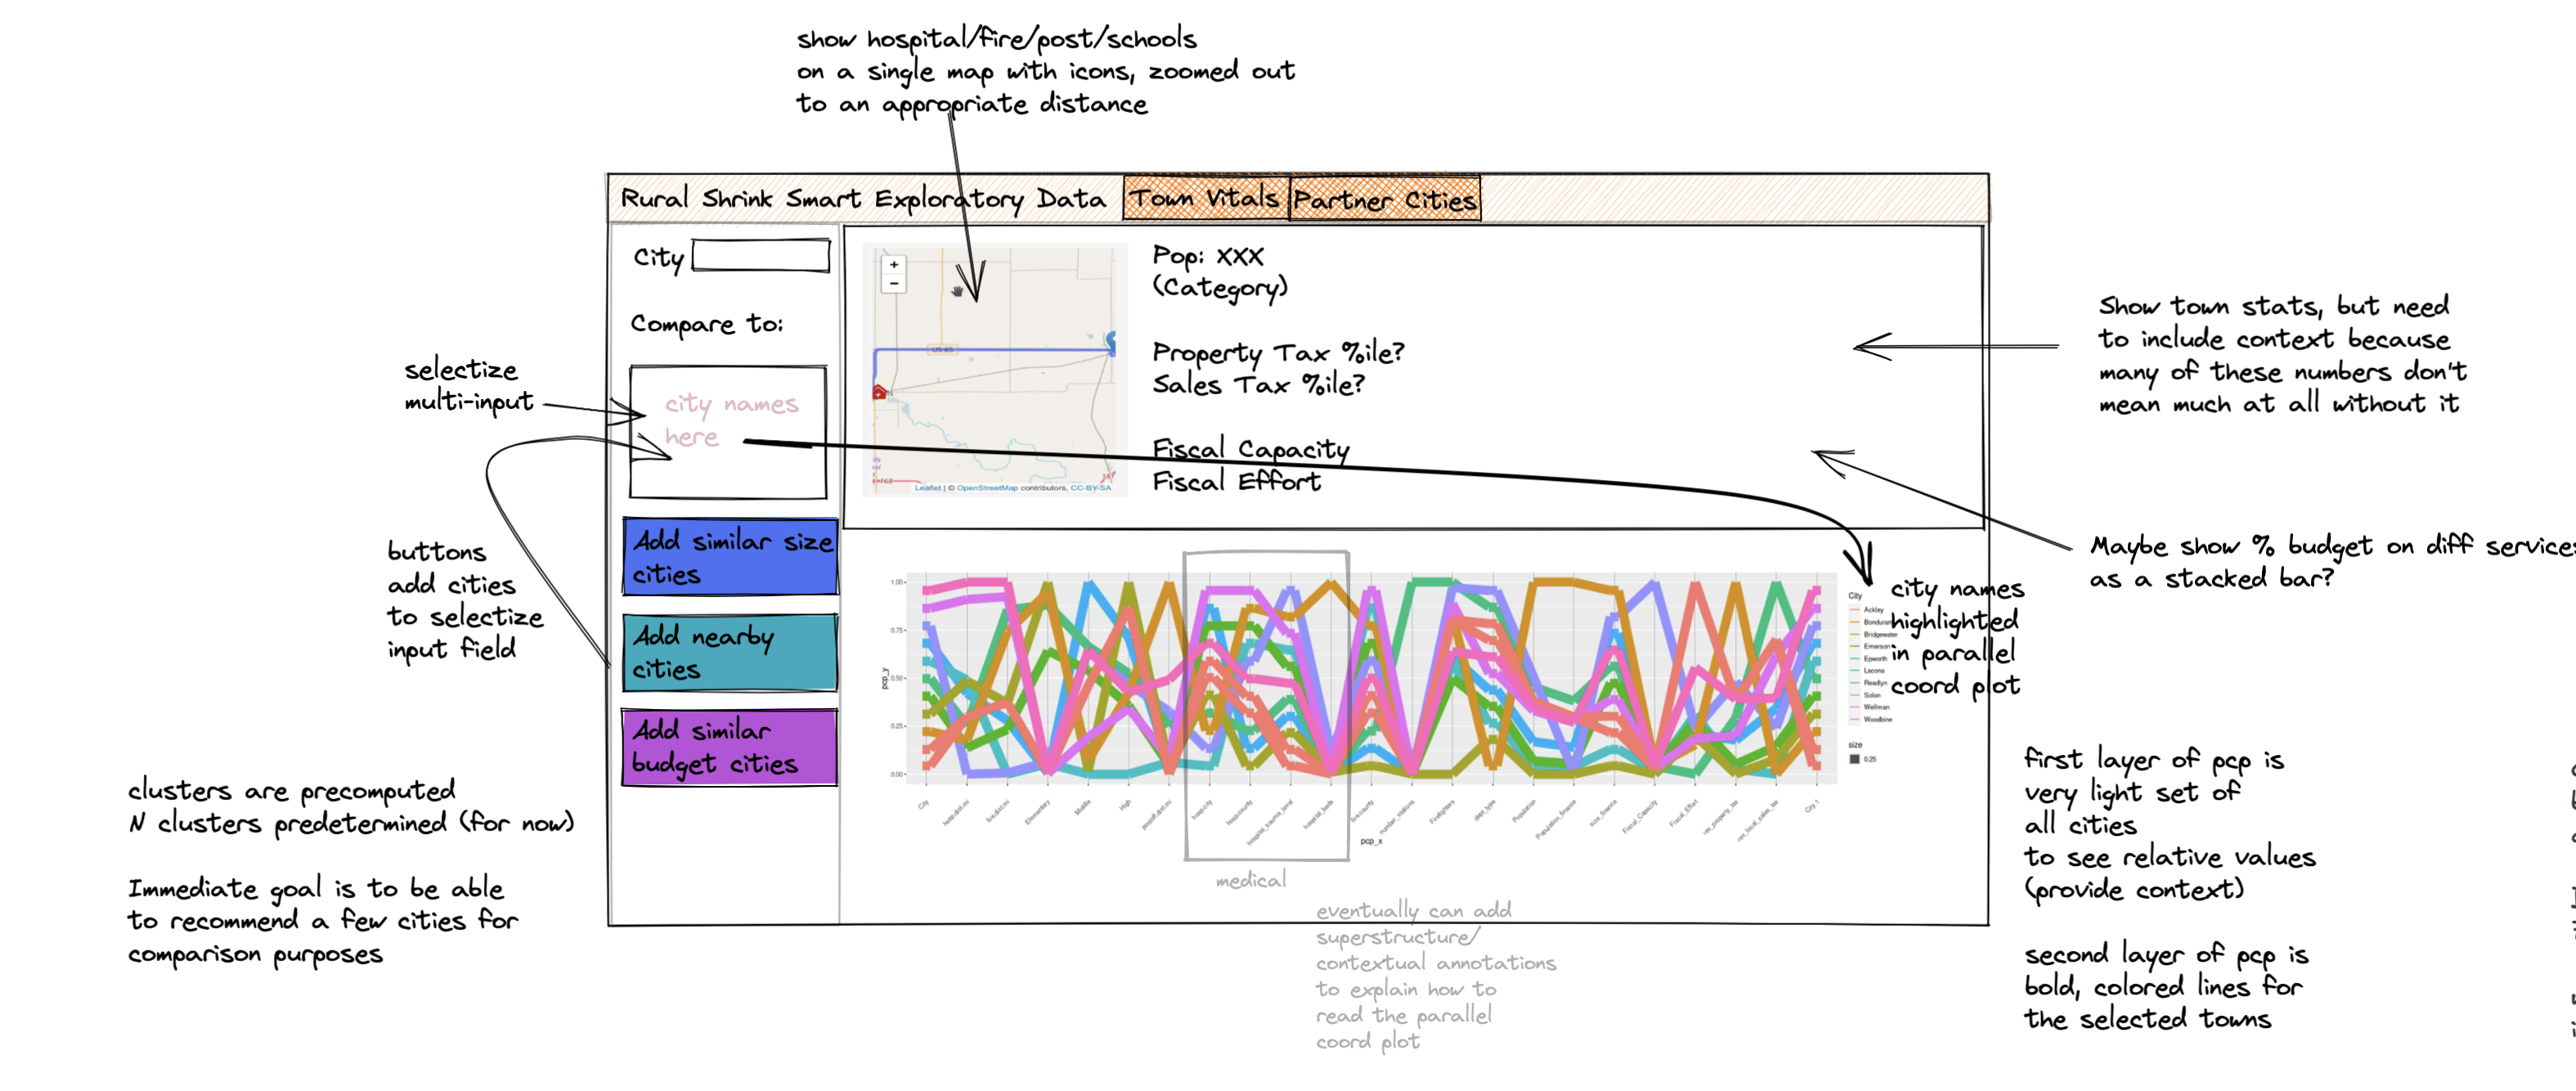
\includegraphics[width=\textwidth]{figure/Version1.png}

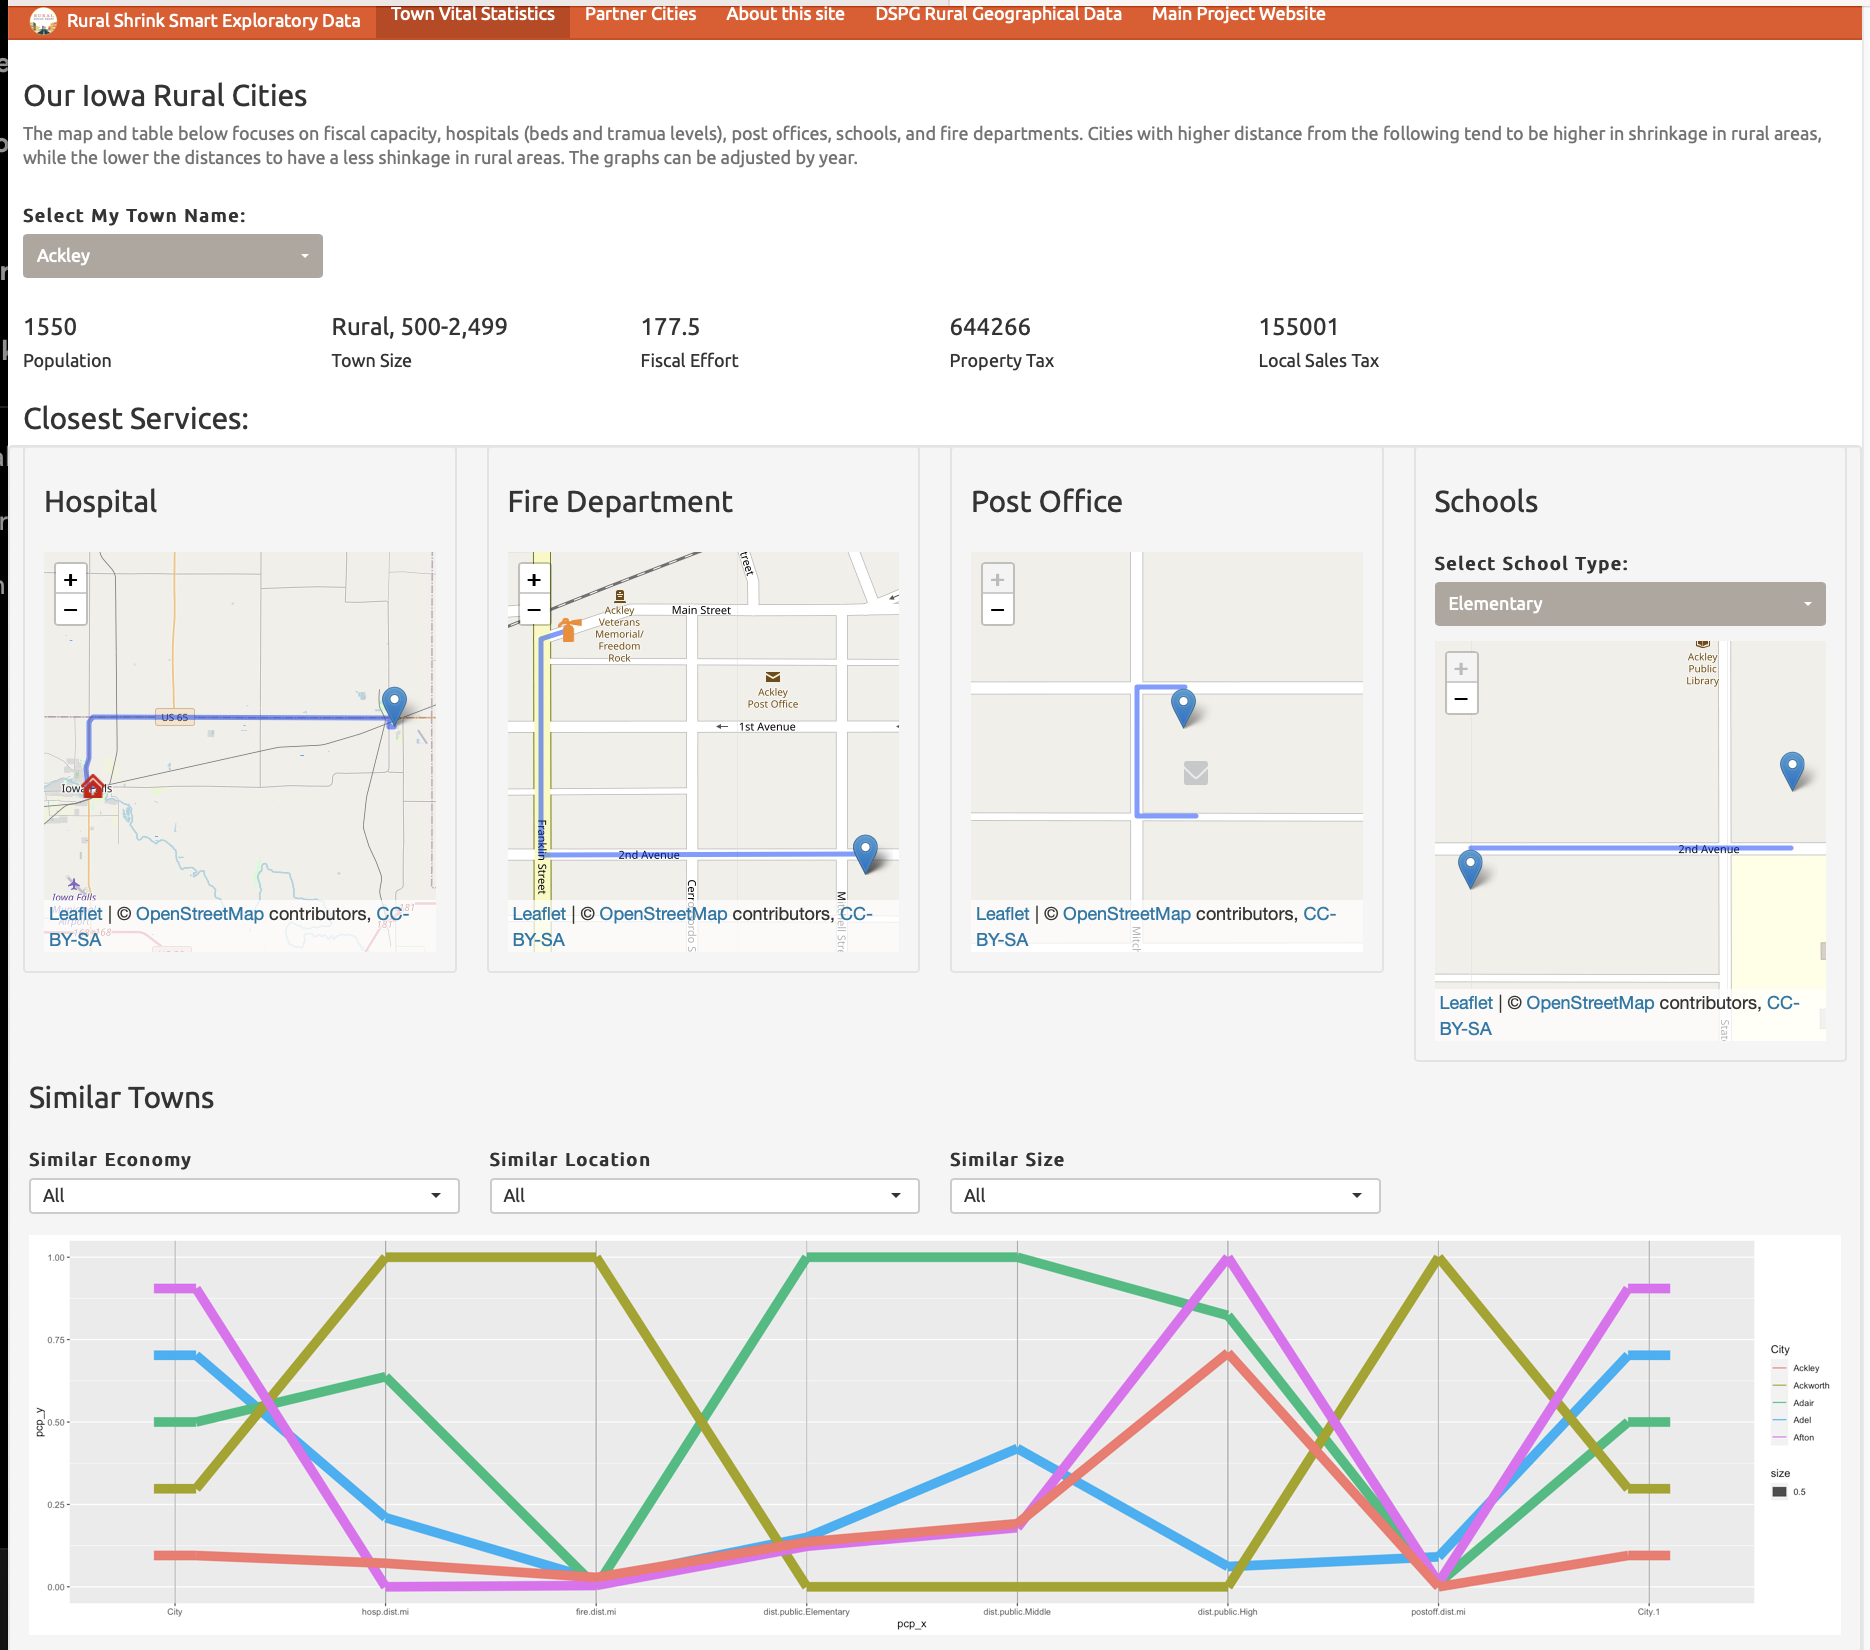
\includegraphics[width=.7\textwidth]{figure/Version2.png}
\caption{Initial dashboard design sketch (top) and implementation (bottom).}\label{fig:v1}
\end{figure}

We implemented some suggested town comparisons using unsupervised clustering methods to help our towns make decisions that are informed in comparison to similar towns, for budget size, population size and location. We initially focused on determining the next five to ten similar towns, based on distances to services. This feature became an important diagnostic for our data quality, as it became clear that towns which were grouped with big cities but which did not have a large population were so grouped because of missing data. Unfortunately, this clustering feature was not as useful to the application users, as they came to the dashboard with a pre-existing set of towns to compare to; our suggested comparisons were in the way.

The initial dashboard design featured several responsive maps showing the distance to the nearest hospital, fire department, post office, and school. These maps were ineffective for several reasons:

\begin{itemize}
\tightlist
\item
  Town residents already know this information (though it was useful for us as the dashboard designers, because we aren't nearly as familiar with the 900+ small towns in Iowa)
\item
  We computed distance from services relative to the center of town - coordinates provided in the data from \url{data.iowa.gov}. Generally speaking, the post office is at the center of town and the fire department is usually very close to the center of town; these two maps were useless. The school and hospital maps were less useless, but still did not provide particularly useful information to people already familiar with the town.
\item
  It became clear that it might be more useful to show the comparison towns on a map (relative to the town of interest) so that users could compare geographical ratings for unfamiliar data to familiar data.
\end{itemize}

In addition, we received feedback on the parallel coordinate plot at the bottom of the app which was surprising: the viewers (in this case, other researchers on the team) were not as intimidated by the parallel coordinate plot as we had expected. They did need some explanation of how to read the plot, and these hints need to be included in the dashboard, but they grasped the fundamental idea of the plot very quickly.

Our conclusion, based on this initial dashboard draft, was that we needed to restructure the application. Our attempt to show familiar information first to ``build up'' to the more unfamiliar structure of a parallel coordinate plot was not effective; there was too much clutter and not enough new information to draw users in.

\subsection{ Redesign }

\begin{figure}
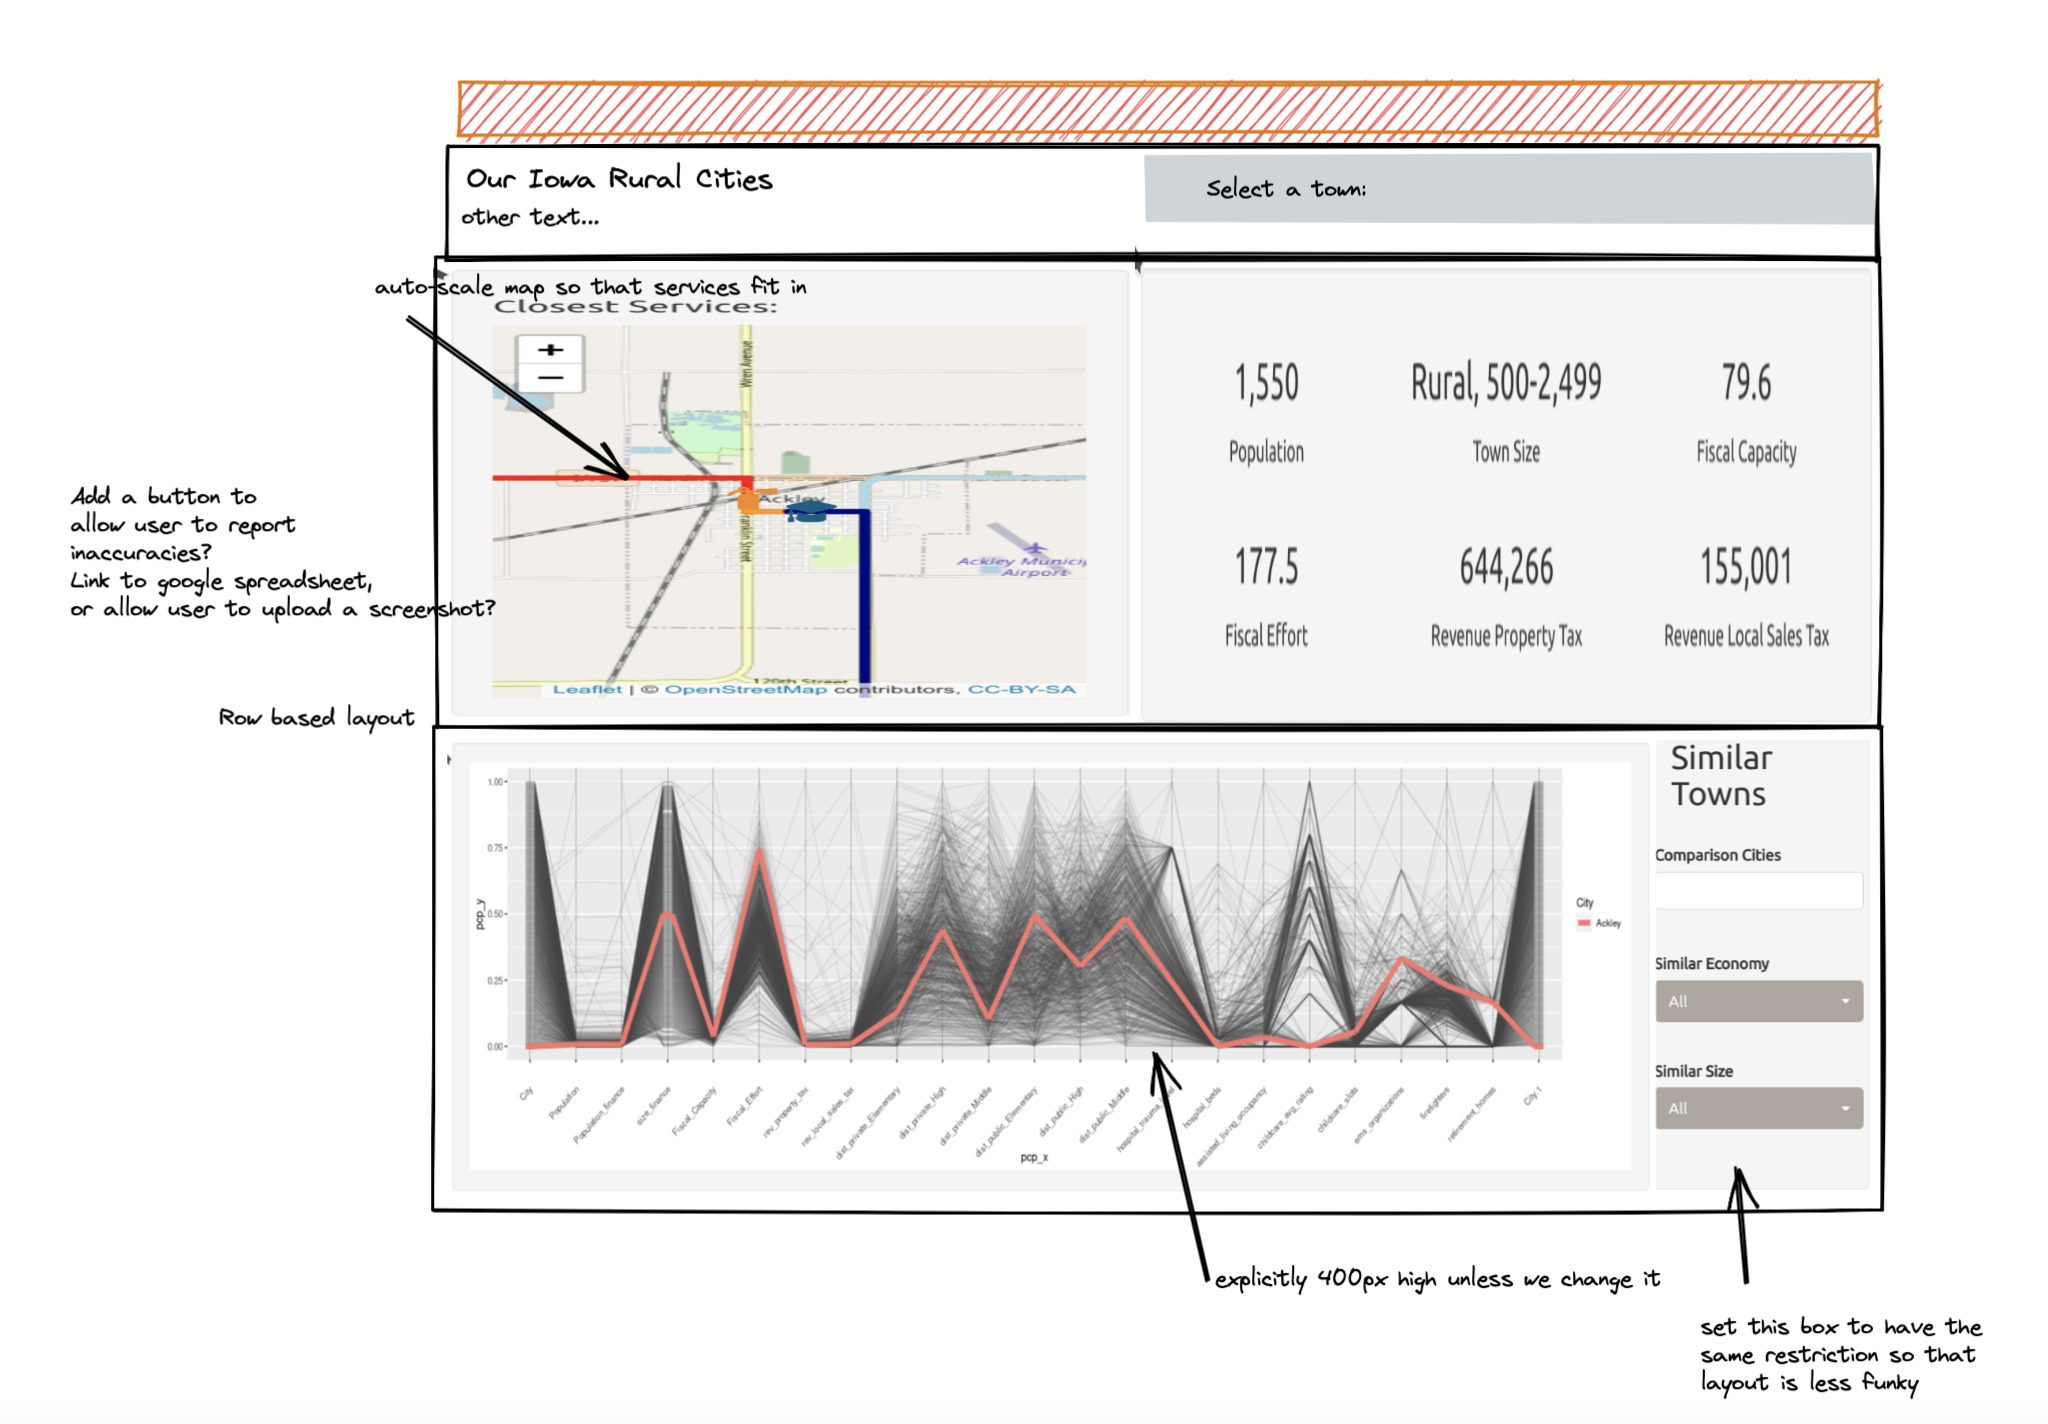
\includegraphics[width=.8\textwidth]{figure/Version3.png}

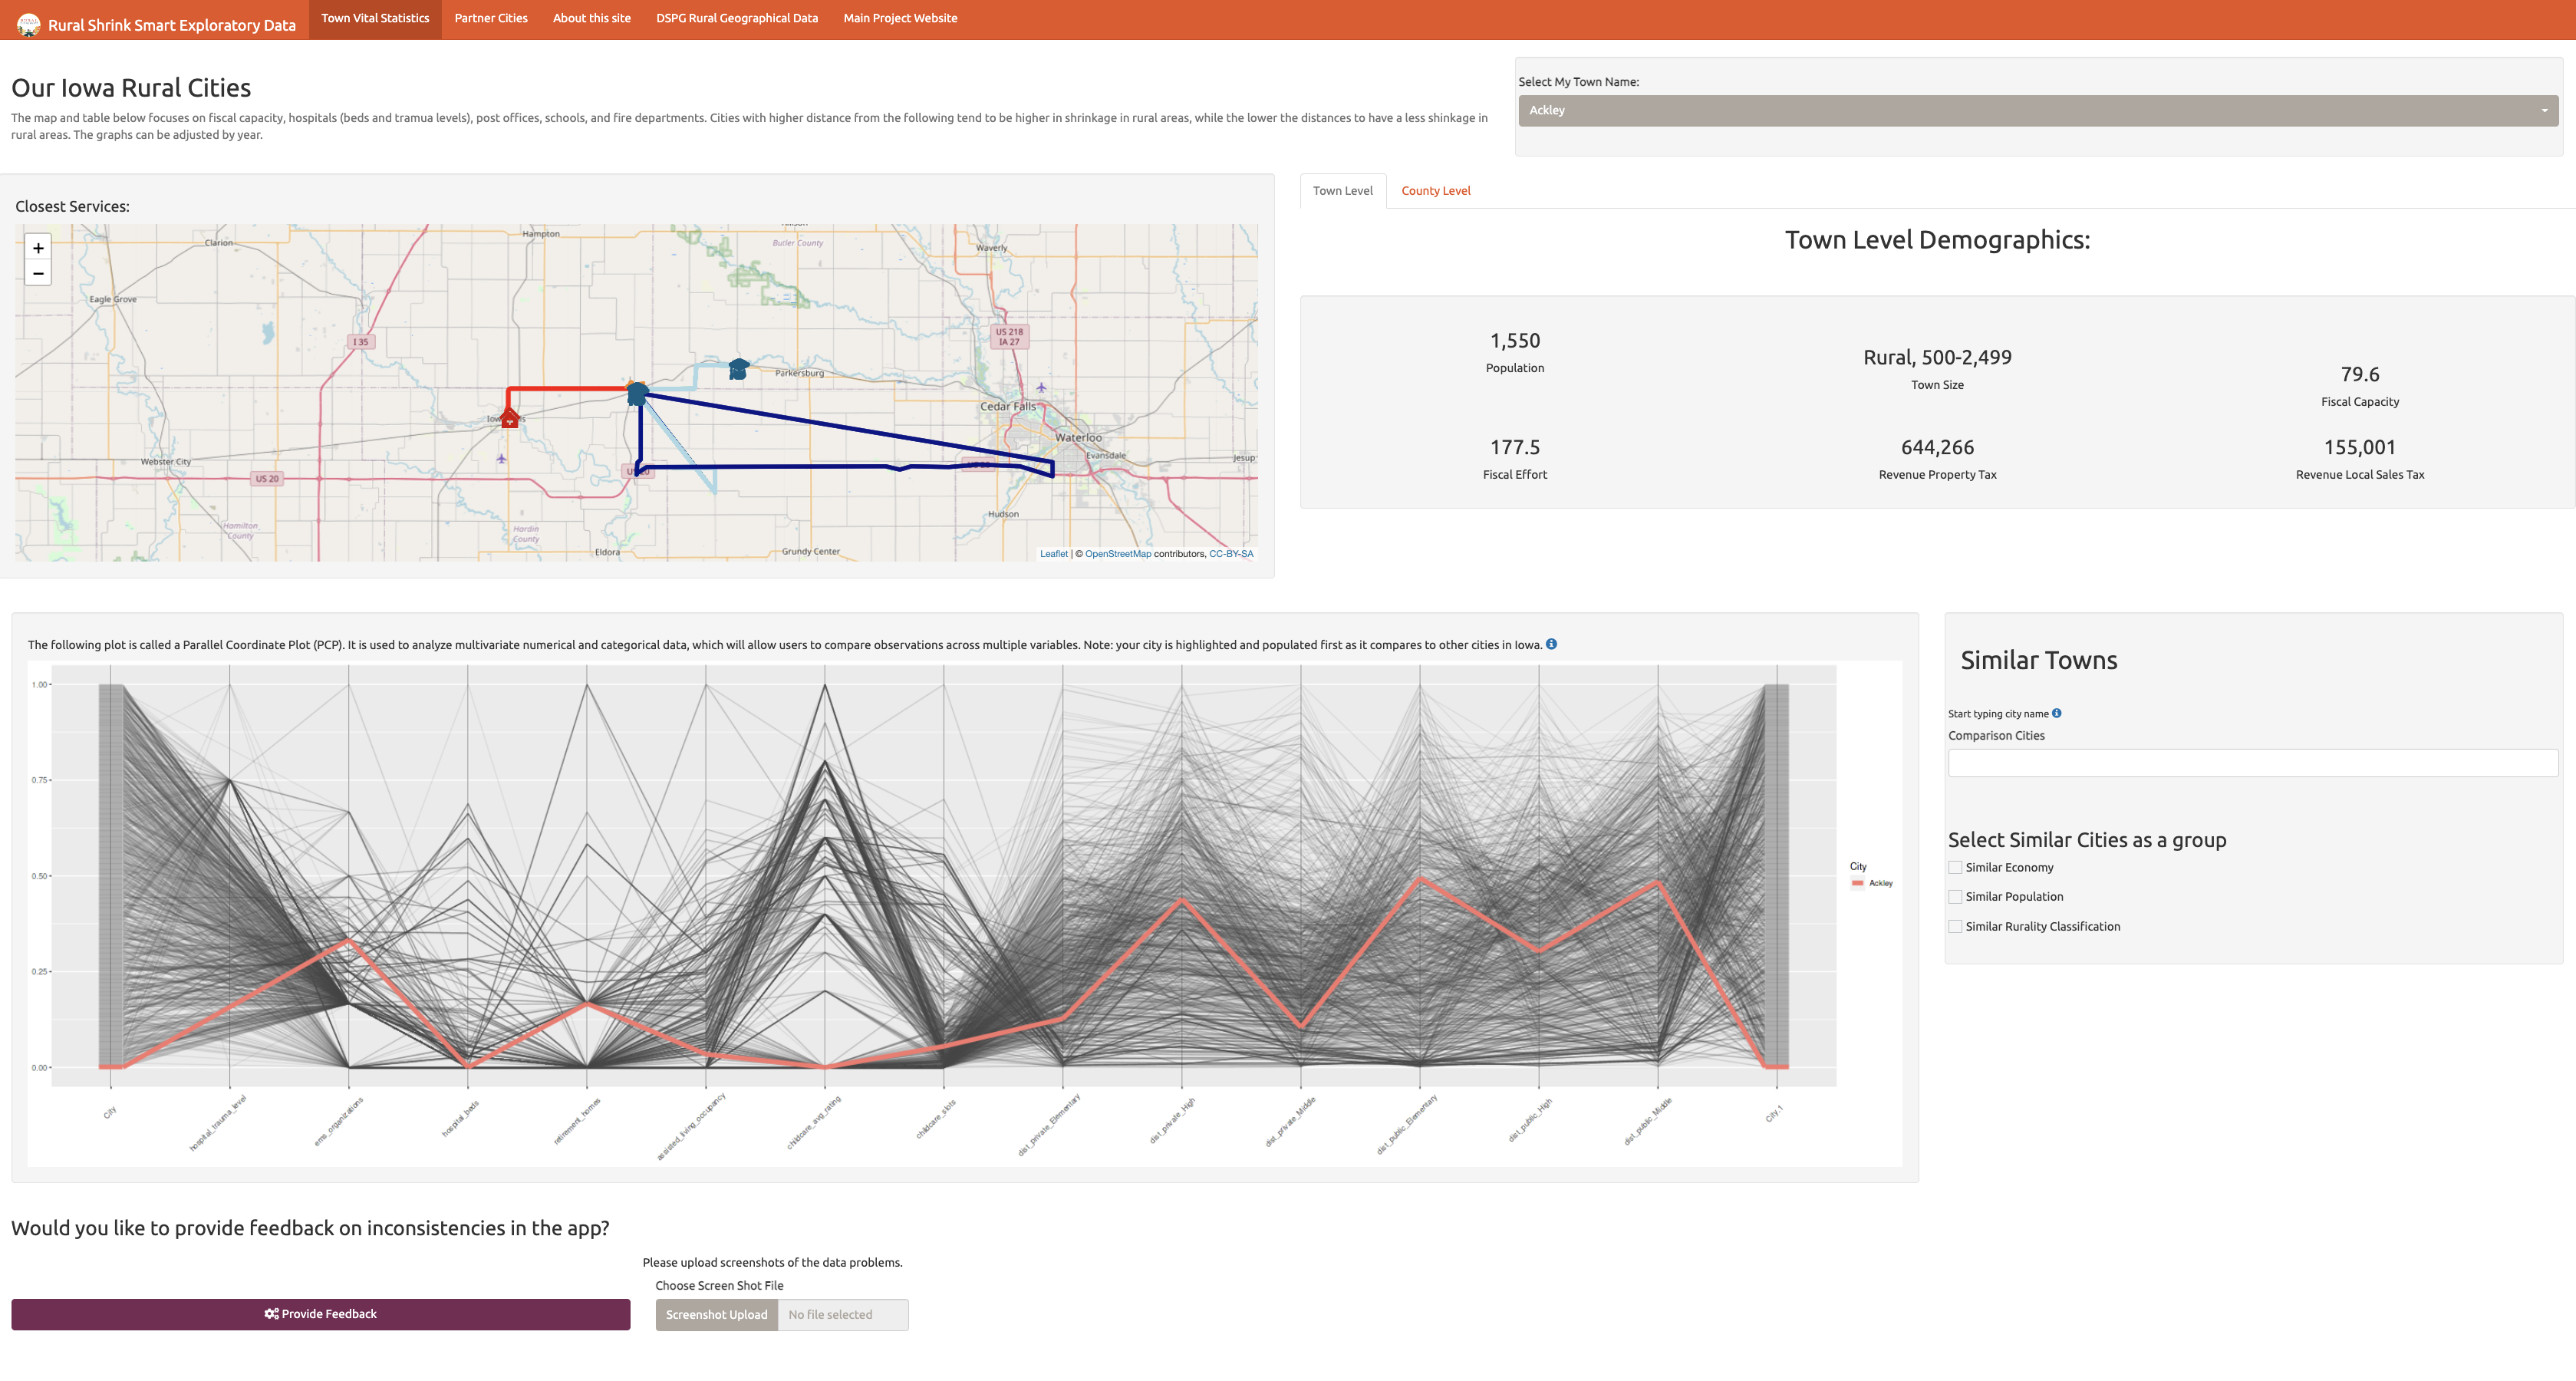
\includegraphics[width=\textwidth]{figure/Version4.png}
\caption{A second iteration of the sketched design (top) and the implementation (bottom).}\label{fig:v2}
\end{figure}

In the initial design, we included a map for each vital service, this initially created a lag for the users' experience. As a result, we cached map directions from OSRM for each service in our database, which drastically reduced the response time for the user. Our initial design did not naturally focus the user's eye on the most important parts of the dashboard; the redesign allowed for a cleaner flow from the top to the bottom.

In addition to the timing due to the map loading slowly, we added the vital statistics at the county level to allow for a more robust understanding of the town and it's surroundings. The rurality index provided a better classification and the USDA sources allowed for the town to understand the impact of the closest major city due to commuting for work and shopping at larger stores not available within the town.

We also modified the parallel coordinate plots in several ways:

\begin{itemize}
\tightlist
\item
  Our x-axis had a large number of variables that we as researchers believed to be the most strongly associated with QoL, grouped into four domains: physical, psychological, social, and environmental. However, there were still too many variables for users to successfully parse. We reduced the number of variables, focusing on variables that had the highest data quality, and we grouped these variables by QoL factor (David J. Peters, 2019).
\item
  Originally, parallel coordinate bands were scaled based on the selected comparison towns. This had the effect of truncating the range of variables and over-emphasizing differences between selected towns relative to the overall range of each variable over all towns in our data set. We chose to show all towns in the data set in a very light \(\alpha\) grey color to provide some information about the overall range of each variable. Unfortunately, even with the low-\(\alpha\) value, this increased the visual complexity of the plot and confused users. Future iterations will likely make use of another aesthetic, such as boxplots or violin plots, to show the range of values for all towns, and then use lines only for towns that are selected by the user. This should strike a balance between visual complexity and representing the data accurately.
\item
  We noticed that users did not make use of our suggested comparison towns, and so we removed that option in favor of allowing users to enter their own comparison towns directly. Users already had pre-determined towns they wanted to compare to, and our suggestions were just in the way.
\end{itemize}

While not all of these modifications were well received in our second round of user testing, the changes did incrementally move the dashboard display towards our goal of allowing users to explore the data and engage with it. We continued to be surprised with how well users reacted to the parallel coordinate plots, which we initially thought might be too abstract for users unfamiliar with multivariate data displays, but the ability to compare towns across multiple dimensions and examine the similarities and differences between their approaches to different services seemed to be intuitive for users once they understood that each vertical axis was a different variable.

\section{ Discussion}

Our dashboard design philosophy worked primarily to promote a town-centric approach application with comparisons to other similar towns being secondary. This approach created a way for the user to see their town information at the top of the page and to explore the PCP after reviewing their own town's essential statistics. The PCP in the lower part of the dashboard allowed for the user to see the plot and adjust to the fact that they could add more towns to the plot, providing an opportunity to explore the wider dataset from a base of familiar knowledge.

While we initially framed the design around guided discovery learning, the approach did not seem to suffice for our user base; instead, we found that users were more drawn to the unfamiliar from the start. We will likely leverage this in future iterations by using visual forms such as flower plots to draw the users in; even though these plots are not ideal for numerical display of data, the visual novelty and aesthetic appeal will provide some motivation to continue exploring and thinking about the data.

One factor that we have briefly considered and have seen hints of in our user feedback is that towns may not want to be compared negatively with other towns. While users have very definite ideas about which towns they would like to compare to, we can always mask the town names and move back to comparisons based on town size and other factors (for instance, whether or not a town is the county seat is a factor that is important outside of population). Using this approach, we would label each town as ``Town 1'', ``Town 2'', and so on, which would eliminate some of the fears about negative comparisons, but would also remove some of the novelty of the data dashboard for our users and would prevent users from drawing on their own outside knowledge about each of the comparison towns.

We also recognize that we need to leverage the expertise of others in our research team: we are working with artists, researchers in architecture, economists, and sociologists; these researchers provide outside knowledge that we do not have and may be able to help us create insightful use-cases to showcase the applet and teach towns how to use it. We can also leverage the app to connect users with our research team, providing additional value to those who use the applet and facilitating development of strategies for maintaining QoL amid shrinking populations.

\section{ Future Work }

One avenue we will explore in future iterations of the dashboard is to incorporate other dashboards generated by different groups within this project. This will create a wider field of information to explore: for instance, some of the additional work will focus on the 99 towns featured in the Iowa Small Town Poll; this will allow us to showcase survey-based measures of quality of life alongside the more objective measurements assembled in the dataset discussed in this paper. While at least one tab of this omni-dashboard will still focus on wider EDA and discovery, we hope to incorporate other information as well to provide a more well-rounded data display encompassing most of the facets of this complex project.

We are also mindful of a distinction between ``eye candy'' and purpose-driven data visualization. While we have typically focused on the latter, there is certainly a place in our dashboard for the former as well. ``Eye candy'' visualization is intended to draw the viewer in and motivate them to explore; while these visualizations may not be particularly effective at communicating quantitative information, if they motivate the user to engage with the rest of the dashboard, they still serve a purpose. It is with this mindset that we intend to explore the use of flower plots - the artistic opportunities combined with the display of quantitative information (even in a form that isn't optimal for quantitative comparisons) may be useful to engage viewers before transitioning to more useful data visualizations intended to provide accurate quantitative comparisons.

EDA can be difficult for a variety of groups of people, novice users and experienced researchers. One of the more difficult components of this project has been clearly articulating the purposes of EDA to a diverse group of researchers unfamiliar with the concept. One of the most useful parts of this dashboard iteration process has been as an aid to data discovery: that is, the dashboard motivated us to find additional data sources and incorporate them into the project. Having conversations with other researchers about the EDA process helped to facilitate these conversations, as each discussion seemed to uncover additional data sources that someone remembered after looking at the dashboard. While this facet of the dashboard process may be difficult to study formally, it would be an interesting avenue for investigation.

\section{Conclusions}

In this paper, we have documented the process of designing a dashboard for exploration and visualization of a large and complex data set assembled from many different sources. Our primary audience was leaders of small towns in Iowa, with a secondary audience of researchers in fields other than statistics collaborating on this project with us. Through the process of revising our dashboard, we found that the idea of guided discovery learning as implemented in our first version did not work as well as we had anticipated. It was more important to focus on allowing users to explore their questions about the dataset by facilitating user-driven comparisons and exploration, rather than attempting to anticipate user desires by providing comparison towns. In addition, we found that it would be more effective to draw users in with novel visual displays, as these seemed to attract more interest than providing known facts and an opportunity to explore outwards from an initial area of familiarity.

While it is hard to apply the findings from one fairly specific visualization project more widely, there is a lack of resources in this area that provide both design philosophies and actual analysis of user feedback in a qualitative sense. We have attempted to address this dearth of information by providing the design strategies, user feedback, and our planned and executed modifications, in the hopes that others facing the daunting challenge of designing a dashboard for EDA may learn something from our experiences.

\hypertarget{ref-labels}{%
\chapter{Tables, Graphics, References, and Labels}\label{ref-labels}}

\hypertarget{tables}{%
\section{Tables}\label{tables}}

By far the easiest way to present tables in your thesis is to store the contents of the table in a CSV or Excel file, then read that file in to your R Markdown document as a data frame. Then you can style the table with the \texttt{kable} function, or functions in the \href{https://cran.r-project.org/web/packages/kableExtra/index.html}{kableExtra} pacakge.

In addition to the tables that can be automatically generated from a data frame in \textbf{R} that you saw in {[}R Markdown Basics{]} using the \texttt{kable} function, you can also create tables using \emph{pandoc}. (More information is available at \url{http://pandoc.org/README.html\#tables}.) This might be useful if you don't have values specifically stored in \textbf{R}, but you'd like to display them in table form. Below is an example. Pay careful attention to the alignment in the table and hyphens to create the rows and columns. Generally I don't recommend this approach of typing the table directly into your R Markdown document.

\begin{longtable}[]{@{}
  >{\centering\arraybackslash}p{(\columnwidth - 4\tabcolsep) * \real{0.3133}}
  >{\centering\arraybackslash}p{(\columnwidth - 4\tabcolsep) * \real{0.5060}}
  >{\centering\arraybackslash}p{(\columnwidth - 4\tabcolsep) * \real{0.1807}}@{}}
\caption{\label{tab:inher} Correlation of Inheritance Factors for Parents and Child}\tabularnewline
\toprule()
\begin{minipage}[b]{\linewidth}\centering
Factors
\end{minipage} & \begin{minipage}[b]{\linewidth}\centering
Correlation between Parents \& Child
\end{minipage} & \begin{minipage}[b]{\linewidth}\centering
Inherited
\end{minipage} \\
\midrule()
\endfirsthead
\toprule()
\begin{minipage}[b]{\linewidth}\centering
Factors
\end{minipage} & \begin{minipage}[b]{\linewidth}\centering
Correlation between Parents \& Child
\end{minipage} & \begin{minipage}[b]{\linewidth}\centering
Inherited
\end{minipage} \\
\midrule()
\endhead
Education & -0.49 & Yes \\
Socio-Economic Status & 0.28 & Slight \\
Income & 0.08 & No \\
Family Size & 0.18 & Slight \\
Occupational Prestige & 0.21 & Slight \\
\bottomrule()
\end{longtable}

We can also create a link to the table by doing the following: Table \ref{tab:inher}. If you go back to {[}Loading and exploring data{]} and look at the \texttt{kable} table, we can create a reference to this max delays table too: Table \ref{tab:maxdelays}. The addition of the \texttt{(\textbackslash{}\#tab:inher)} option to the end of the table caption allows us to then make a reference to Table \texttt{\textbackslash{}@ref(tab:label)}. Note that this reference could appear anywhere throughout the document after the table has appeared.

\clearpage

\hypertarget{figures}{%
\section{Figures}\label{figures}}

If your thesis has a lot of figures, \emph{R Markdown} might behave better for you than that other word processor. One perk is that it will automatically number the figures accordingly in each chapter. You'll also be able to create a label for each figure, add a caption, and then reference the figure in a way similar to what we saw with tables earlier. If you label your figures, you can move the figures around and \emph{R Markdown} will automatically adjust the numbering for you. No need for you to remember! So that you don't have to get too far into LaTeX to do this, a couple \textbf{R} functions have been created for you to assist. You'll see their use below.

In the \textbf{R} chunk below, we will load in a picture stored as \texttt{uw.png} in our main directory. We then give it the caption of ``UW logo'', the label of ``uwlogo'', and specify that this is a figure. Make note of the different \textbf{R} chunk options that are given in the R Markdown file (not shown in the knitted document).

\begin{Shaded}
\begin{Highlighting}[]
\FunctionTok{include\_graphics}\NormalTok{(}\AttributeTok{path =} \StringTok{"figure/unl.png"}\NormalTok{)}
\end{Highlighting}
\end{Shaded}

\begin{figure}

\includegraphics[width=\linewidth]{figure/unl} \caption{logo}\label{fig:uwlogo}
\end{figure}

Here is a reference to the UW logo: Figure \ref{fig:uwlogo}. Note the use of the \texttt{fig:} code here. By naming the \textbf{R} chunk that contains the figure, we can then reference that figure later as done in the first sentence here. We can also specify the caption for the figure via the R chunk option \texttt{fig.cap}.

\clearpage

Below we will investigate how to save the output of an \textbf{R} plot and label it in a way similar to that done above. Recall the \texttt{flights} dataset from Chapter \ref{rmd-basics}. (Note that we've shown a different way to reference a section or chapter here.) We will next explore a bar graph with the mean flight departure delays by airline from Portland for 2014. Note also the use of the \texttt{scale} parameter which is discussed on the next page.

\begin{Shaded}
\begin{Highlighting}[]
\FunctionTok{library}\NormalTok{(nycflights13)}
\FunctionTok{data}\NormalTok{(flights)}
\NormalTok{flights }\SpecialCharTok{\%\textgreater{}\%}
    \FunctionTok{group\_by}\NormalTok{(carrier) }\SpecialCharTok{\%\textgreater{}\%}
    \FunctionTok{summarize}\NormalTok{(}\AttributeTok{mean\_dep\_delay =} \FunctionTok{mean}\NormalTok{(dep\_delay)) }\SpecialCharTok{\%\textgreater{}\%}
    \FunctionTok{ggplot}\NormalTok{(}\FunctionTok{aes}\NormalTok{(}\AttributeTok{x =}\NormalTok{ carrier, }\AttributeTok{y =}\NormalTok{ mean\_dep\_delay)) }\SpecialCharTok{+}
    \FunctionTok{geom\_bar}\NormalTok{(}\AttributeTok{position =} \StringTok{"identity"}\NormalTok{, }\AttributeTok{stat =} \StringTok{"identity"}\NormalTok{,}
        \AttributeTok{fill =} \StringTok{"red"}\NormalTok{)}
\end{Highlighting}
\end{Shaded}

\begin{verbatim}
## Warning: Removed 15 rows containing
## missing values
## (`geom_bar()`).
\end{verbatim}

\begin{figure}
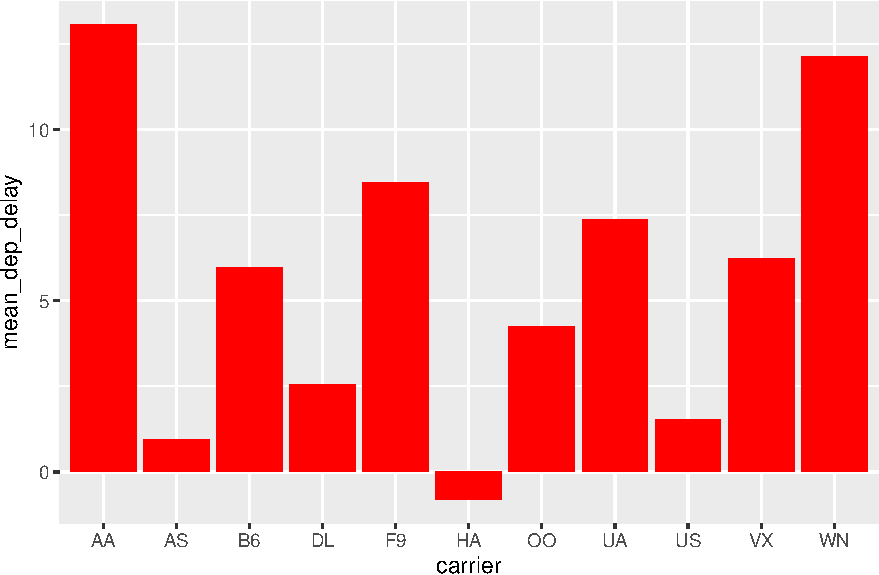
\includegraphics[width=\linewidth]{thesis_files/figure-latex/delaysboxplot-1} \caption{Mean Delays by Airline}\label{fig:delaysboxplot}
\end{figure}

Here is a reference to this image: Figure \ref{fig:delaysboxplot}.

A table linking these carrier codes to airline names is available at \url{https://github.com/ismayc/pnwflights14/blob/master/data/airlines.csv}.

\clearpage

Next, we will explore the use of the \texttt{out.extra} chunk option, which can be used to shrink or expand an image loaded from a file by specifying \texttt{"scale=\ "}. Here we use the mathematical graph stored in the ``subdivision.pdf'' file.

\begin{figure}
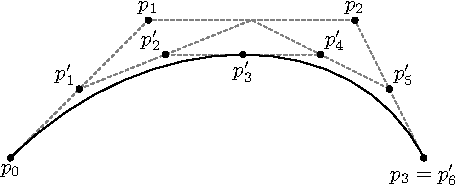
\includegraphics[width=\linewidth,scale=0.75]{figure/subdivision} \caption{Subdiv. graph}\label{fig:subd}
\end{figure}

Here is a reference to this image: Figure \ref{fig:subd}. Note that \texttt{echo=FALSE} is specified so that the \textbf{R} code is hidden in the document.

\textbf{More Figure Stuff}

Lastly, we will explore how to rotate and enlarge figures using the \texttt{out.extra} chunk option. (Currently this only works in the PDF version of the book.)

\begin{figure}
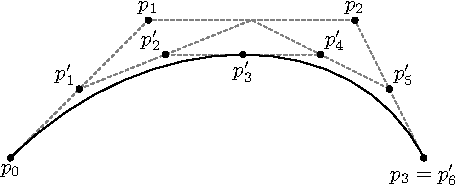
\includegraphics[width=\linewidth,angle=180, scale=1.1]{figure/subdivision} \caption{A Larger Figure, Flipped Upside Down}\label{fig:subd2}
\end{figure}

As another example, here is a reference: Figure \ref{fig:subd2}.

\hypertarget{footnotes-and-endnotes}{%
\section{Footnotes and Endnotes}\label{footnotes-and-endnotes}}

You might want to footnote something. \footnote{footnote text} The footnote will be in a smaller font and placed appropriately. Endnotes work in much the same way.

\hypertarget{cross-referencing-chapters-and-sections}{%
\section{Cross-referencing chapters and sections}\label{cross-referencing-chapters-and-sections}}

The \href{https://bookdown.org/yihui/bookdown/cross-references.html}{bookdown documentation} is an excellent source for learning how to cross-reference in a bookdown project such as a huskydown document. Here we only cover the most common uses for a typical thesis. If you want something more complex or fancy, please refer to the bookdown documentation and seek help from the developers of that package.

By default, all of your chapter and section headers will get an auto-generated ID label For example, e.g., \texttt{\#\ Chapter\ 1} will have an auto-generated ID \texttt{chapter-1}. Note that the ID label is all lower case, and has no spaces. If you have any kind of punctuation in your header, such as a colon (:), it will not appear in the ID label. Then in your text you can reference chapter one in your Rmd file like this: `as discussed in Chapter \texttt{\textbackslash{}@ref(chapter-1)}', which will print as `as discussed in Chapter 1'

We strongly recommend that you to manually assign ID labels to your chapter header to make it easy to cross-reference. For example, at the top of the Rmd file for this chapter, you can see:

\texttt{\#\ Tables,\ Graphics,\ References,\ and\ Labels\ \{\#ref-labels\}}

The \texttt{\{\#ref-labels\}} part of this header is the ID label. It doesn't show in the output, but is there for us to use for easy cross-referencing, because it can be short, and we don't need to change it elsewhere our document when we update the chapter header. We can use this custom ID label in our Rmd document like this: `as discussed in Chapter \texttt{\textbackslash{}@ref(ref-labels)}', which will print as `as discussed in Chapter \ref{ref-labels}'. If you need to show custom text instead of the chapter number, you use this syntax in your Rmd document: \texttt{see\ {[}my\ chapter\ about\ labels{]}(\#ref-labels)\ for\ more\ details} which will appear as `see \protect\hyperlink{ref-labels}{my chapter about labels} for more details'

To cross-reference a specific section in the same chapter, we recommend adding a custom ID label to the section header, and using that to cross-reference. For example, earlier in this chapter we have a section on tables and in the Rmd file we see \texttt{\#\#\ Tables\ \{\#tables\}}. We can cross-reference that in the text like this `as discussed in the section on \texttt{{[}tables{]}(\#tables)}' which will appear as `as discussed in the above section on \protect\hyperlink{tables}{tables}'

To cross-reference a section in a different chapter we can use the ID label from that section directly. For example, we can write in our Rmd document \texttt{as\ discussed\ in\ the\ section\ on\ {[}R\ code\ chunks{]}(\#r-chunks)\ in\ Chapter\ \textbackslash{}@ref(rmd-basics)} which will appear as `as discussed in the section on \protect\hyperlink{r-chunks}{R code chunks} in Chapter \ref{rmd-basics}'.

If you prefer to cross-reference by the section number, we can use custom ID labels in our Rmd document. For example, to refer to a section in our first chapter, we can write in the Rmd document: \texttt{as\ discussed\ in\ section\ \textbackslash{}@ref(r-chunks)\ in\ Chapter\ \textbackslash{}@ref(rmd-basics)}. This will appear with section and chapter numbers like so: as `as discussed in section \ref{r-chunks} in Chapter \ref{rmd-basics}'.

\hypertarget{bibliographies}{%
\section{Bibliographies}\label{bibliographies}}

Of course you will need to cite things, and you will probably accumulate an armful of sources. There are a variety of tools available for creating a bibliography database (stored with the .bib extension). In addition to BibTeX suggested below, you may want to consider using the free and easy-to-use tool called Zotero. Some Zotero documentation is at \url{http://libguides.reed.edu/citation/zotero}. In addition, a tutorial is available from Middlebury College at \url{http://sites.middlebury.edu/zoteromiddlebury/}.

\emph{R Markdown} uses \emph{pandoc} (\url{http://pandoc.org/}) to build its bibliographies. One nice caveat of this is that you won't have to do a second compile to load in references as standard LaTeX requires. To cite references in your thesis (after creating your bibliography database), place the reference name inside square brackets and precede it by the ``at'' symbol. For example, here's a reference to a book about worrying: (Molina \& Borkovec, 1994). This \texttt{Molina1994} entry appears in a file called \texttt{thesis.bib} in the \texttt{bib} folder. This bibliography database file was created by a program called BibTeX. You can call this file something else if you like (look at the YAML header in the main .Rmd file) and, by default, is to placed in the \texttt{bib} folder.

For more information about BibTeX and bibliographies, see (\url{http://web.reed.edu/cis/help/latex/index.html})\footnote{Reed~College (2007)}. There are three pages on this topic: \emph{bibtex} (which talks about using BibTeX, at \url{http://web.reed.edu/cis/help/latex/bibtex.html}), \emph{bibtexstyles} (about how to find and use the bibliography style that best suits your needs, at \url{http://web.reed.edu/cis/help/latex/bibtexstyles.html}) and \emph{bibman} (which covers how to make and maintain a bibliography by hand, without BibTeX, at \url{http://web.reed.edu/cis/help/latex/bibman.html}). The last page will not be useful unless you have only a few sources.

If you look at the YAML header at the top of the main .Rmd file you can see that we can specify the style of the bibliography by referencing the appropriate csl file. You can download a variety of different style files at \url{https://www.zotero.org/styles}. Make sure to download the file into the csl folder.

\textbf{Tips for Bibliographies}

\begin{itemize}
\tightlist
\item
  Like with thesis formatting, the sooner you start compiling your bibliography for something as large as thesis, the better.
\item
  The cite key (a citation's label) needs to be unique from the other entries.
\item
  When you have more than one author or editor, you need to separate each author's name by the word ``and'' e.g.~\texttt{Author\ =\ \{Noble,\ Sam\ and\ Youngberg,\ Jessica\},}.
\item
  Bibliographies made using BibTeX (whether manually or using a manager) accept LaTeX markup, so you can italicize and add symbols as necessary.
\item
  To force capitalization in an article title or where all lowercase is generally used, bracket the capital letter in curly braces.
\end{itemize}

\hypertarget{anything-else}{%
\section{Anything else?}\label{anything-else}}

If you'd like to see examples of other things in this template, please \href{https://github.com/benmarwick/huskydown/issues/new}{contact us} (email \href{mailto:bmarwick@uw.edu}{\nolinkurl{bmarwick@uw.edu}}) with your suggestions. We love to see people using \emph{R Markdown} for their theses, and are happy to help.

\hypertarget{conclusion-1}{%
\chapter*{Conclusion}\label{conclusion-1}}
\addcontentsline{toc}{chapter}{Conclusion}

If we don't want Conclusion to have a chapter number next to it, we can add the \texttt{\{-\}} attribute.

\textbf{More info}

And here's some other random info: the first paragraph after a chapter title or section head \emph{shouldn't be} indented, because indents are to tell the reader that you're starting a new paragraph. Since that's obvious after a chapter or section title, proper typesetting doesn't add an indent there.

\appendix

\hypertarget{the-first-appendix}{%
\chapter{The First Appendix}\label{the-first-appendix}}

This first appendix includes all of the R chunks of code that were hidden throughout the document (using the \texttt{include\ =\ FALSE} chunk tag) to help with readibility and/or setup.

\textbf{In the main Rmd file}

\begin{Shaded}
\begin{Highlighting}[]
\FunctionTok{library}\NormalTok{(knitr)}
\FunctionTok{library}\NormalTok{(palmerpenguins)}
\FunctionTok{library}\NormalTok{(tidyverse)}
\FunctionTok{library}\NormalTok{(nycflights13)}
\FunctionTok{data}\NormalTok{(flights)}

\FunctionTok{library}\NormalTok{(ggpcp)}
\FunctionTok{library}\NormalTok{(ggplot2)}
\FunctionTok{library}\NormalTok{(dplyr)}
\FunctionTok{data}\NormalTok{(nasa)}

\FunctionTok{library}\NormalTok{(scales)}
\FunctionTok{library}\NormalTok{(datasets)}
\FunctionTok{data}\NormalTok{(}\StringTok{"ChickWeight"}\NormalTok{)}
\FunctionTok{library}\NormalTok{(formatR)}
\end{Highlighting}
\end{Shaded}

\textbf{In Chapter \ref{ref-labels}:}

\hypertarget{the-second-appendix-for-fun}{%
\chapter{The Second Appendix, for Fun}\label{the-second-appendix-for-fun}}

\hypertarget{colophon}{%
\chapter*{Colophon}\label{colophon}}
\addcontentsline{toc}{chapter}{Colophon}

This document is set in \href{https://github.com/georgd/EB-Garamond}{EB Garamond}, \href{https://github.com/adobe-fonts/source-code-pro/}{Source Code Pro} and \href{http://www.latofonts.com/lato-free-fonts/}{Lato}. The body text is set at 11pt with \(\familydefault\).

It was written in R Markdown and \(\LaTeX\), and rendered into PDF using \href{https://github.com/benmarwick/huskydown}{huskydown} and \href{https://github.com/rstudio/bookdown}{bookdown}.

This document was typeset using the XeTeX typesetting system, and the \href{http://staff.washington.edu/fox/tex/}{University of Washington Thesis class} class created by Jim Fox. Under the hood, the \href{https://github.com/UWIT-IAM/UWThesis}{University of Washington Thesis LaTeX template} is used to ensure that documents conform precisely to submission standards. Other elements of the document formatting source code have been taken from the \href{https://github.com/stevenpollack/ucbthesis}{Latex, Knitr, and RMarkdown templates for UC Berkeley's graduate thesis}, and \href{https://github.com/suchow/Dissertate}{Dissertate: a LaTeX dissertation template to support the production and typesetting of a PhD dissertation at Harvard, Princeton, and NYU}

The source files for this thesis, along with all the data files, have been organised into an R package, xxx, which is available at \url{https://github.com/xxx/xxx}. A hard copy of the thesis can be found in the University of Washington library.

This version of the thesis was generated on 2023-04-09 12:49:33. The repository is currently at this commit:

The computational environment that was used to generate this version is as follows:

\begin{verbatim}
## - Session info -------------
##  setting  value
##  version  R version 4.2.2 (2022-10-31)
##  os       macOS Big Sur ... 10.16
##  system   x86_64, darwin17.0
##  ui       X11
##  language (EN)
##  collate  en_US.UTF-8
##  ctype    en_US.UTF-8
##  tz       America/New_York
##  date     2023-04-09
##  pandoc   2.19.2 @ /Applications/RStudio.app/Contents/Resources/app/quarto/bin/tools/ (via rmarkdown)
## 
## - Packages -----------------
##  package        * version date (UTC) lib source
##  assertthat       0.2.1   2019-03-21 [1] CRAN (R 4.2.0)
##  bookdown         0.33    2023-03-06 [1] CRAN (R 4.2.0)
##  cachem           1.0.7   2023-02-24 [1] CRAN (R 4.2.0)
##  callr            3.7.3   2022-11-02 [1] CRAN (R 4.2.0)
##  cli              3.6.0   2023-01-09 [1] CRAN (R 4.2.0)
##  colorspace       2.1-0   2023-01-23 [1] CRAN (R 4.2.0)
##  crayon           1.5.2   2022-09-29 [1] CRAN (R 4.2.0)
##  devtools         2.4.5   2022-10-11 [1] CRAN (R 4.2.0)
##  digest           0.6.31  2022-12-11 [1] CRAN (R 4.2.0)
##  dplyr          * 1.1.1   2023-03-22 [1] CRAN (R 4.2.0)
##  ellipsis         0.3.2   2021-04-29 [1] CRAN (R 4.2.0)
##  evaluate         0.20    2023-01-17 [1] CRAN (R 4.2.0)
##  fansi            1.0.4   2023-01-22 [1] CRAN (R 4.2.0)
##  farver           2.1.1   2022-07-06 [1] CRAN (R 4.2.0)
##  fastmap          1.1.1   2023-02-24 [1] CRAN (R 4.2.0)
##  forcats        * 1.0.0   2023-01-29 [1] CRAN (R 4.2.0)
##  formatR        * 1.14    2023-01-17 [1] CRAN (R 4.2.0)
##  fs               1.6.1   2023-02-06 [1] CRAN (R 4.2.0)
##  generics         0.1.3   2022-07-05 [1] CRAN (R 4.2.0)
##  ggpcp          * 0.2.0   2022-11-28 [1] CRAN (R 4.2.0)
##  ggplot2        * 3.4.1   2023-02-10 [1] CRAN (R 4.2.0)
##  glue             1.6.2   2022-02-24 [1] CRAN (R 4.2.0)
##  gtable           0.3.3   2023-03-21 [1] CRAN (R 4.2.0)
##  hms              1.1.3   2023-03-21 [1] CRAN (R 4.2.0)
##  htmltools        0.5.4   2022-12-07 [1] CRAN (R 4.2.0)
##  htmlwidgets      1.6.2   2023-03-17 [1] CRAN (R 4.2.0)
##  httpuv           1.6.9   2023-02-14 [1] CRAN (R 4.2.0)
##  knitr          * 1.42    2023-01-25 [1] CRAN (R 4.2.0)
##  labeling         0.4.2   2020-10-20 [1] CRAN (R 4.2.0)
##  later            1.3.0   2021-08-18 [1] CRAN (R 4.2.0)
##  lifecycle        1.0.3   2022-10-07 [1] CRAN (R 4.2.0)
##  lubridate      * 1.9.2   2023-02-10 [1] CRAN (R 4.2.0)
##  magrittr         2.0.3   2022-03-30 [1] CRAN (R 4.2.0)
##  memoise          2.0.1   2021-11-26 [1] CRAN (R 4.2.0)
##  mime             0.12    2021-09-28 [1] CRAN (R 4.2.0)
##  miniUI           0.1.1.1 2018-05-18 [1] CRAN (R 4.2.0)
##  munsell          0.5.0   2018-06-12 [1] CRAN (R 4.2.0)
##  nycflights13   * 1.0.2   2021-04-12 [1] CRAN (R 4.2.0)
##  palmerpenguins * 0.1.1   2022-08-15 [1] CRAN (R 4.2.0)
##  pillar           1.9.0   2023-03-22 [1] CRAN (R 4.2.2)
##  pkgbuild         1.4.0   2022-11-27 [1] CRAN (R 4.2.0)
##  pkgconfig        2.0.3   2019-09-22 [1] CRAN (R 4.2.0)
##  pkgload          1.3.2   2022-11-16 [1] CRAN (R 4.2.0)
##  prettyunits      1.1.1   2020-01-24 [1] CRAN (R 4.2.0)
##  processx         3.8.0   2022-10-26 [1] CRAN (R 4.2.0)
##  profvis          0.3.7   2020-11-02 [1] CRAN (R 4.2.0)
##  promises         1.2.0.1 2021-02-11 [1] CRAN (R 4.2.0)
##  ps               1.7.4   2023-04-02 [1] CRAN (R 4.2.0)
##  purrr          * 1.0.1   2023-01-10 [1] CRAN (R 4.2.0)
##  R6               2.5.1   2021-08-19 [1] CRAN (R 4.2.0)
##  RColorBrewer     1.1-3   2022-04-03 [1] CRAN (R 4.2.0)
##  Rcpp             1.0.10  2023-01-22 [1] CRAN (R 4.2.0)
##  readr          * 2.1.4   2023-02-10 [1] CRAN (R 4.2.0)
##  remotes          2.4.2   2021-11-30 [1] CRAN (R 4.2.0)
##  rlang            1.1.0   2023-03-14 [1] CRAN (R 4.2.0)
##  rmarkdown        2.20    2023-01-19 [1] CRAN (R 4.2.2)
##  rstudioapi       0.14    2022-08-22 [1] CRAN (R 4.2.0)
##  scales         * 1.2.1   2022-08-20 [1] CRAN (R 4.2.0)
##  sessioninfo      1.2.2   2021-12-06 [1] CRAN (R 4.2.0)
##  shiny            1.7.4   2022-12-15 [1] CRAN (R 4.2.0)
##  stringi          1.7.12  2023-01-11 [1] CRAN (R 4.2.0)
##  stringr        * 1.5.0   2022-12-02 [1] CRAN (R 4.2.0)
##  tibble         * 3.2.1   2023-03-20 [1] CRAN (R 4.2.0)
##  tidyr          * 1.3.0   2023-01-24 [1] CRAN (R 4.2.0)
##  tidyselect       1.2.0   2022-10-10 [1] CRAN (R 4.2.0)
##  tidyverse      * 2.0.0   2023-02-22 [1] CRAN (R 4.2.0)
##  timechange       0.2.0   2023-01-11 [1] CRAN (R 4.2.0)
##  tzdb             0.3.0   2022-03-28 [1] CRAN (R 4.2.0)
##  urlchecker       1.0.1   2021-11-30 [1] CRAN (R 4.2.0)
##  usethis          2.1.6   2022-05-25 [1] CRAN (R 4.2.0)
##  utf8             1.2.3   2023-01-31 [1] CRAN (R 4.2.0)
##  vctrs            0.6.1   2023-03-22 [1] CRAN (R 4.2.0)
##  withr            2.5.0   2022-03-03 [1] CRAN (R 4.2.0)
##  xfun             0.37    2023-01-31 [1] CRAN (R 4.2.0)
##  xtable           1.8-4   2019-04-21 [1] CRAN (R 4.2.0)
##  yaml             2.3.7   2023-01-23 [1] CRAN (R 4.2.0)
## 
##  [1] /Library/Frameworks/R.framework/Versions/4.2/Resources/library
## 
## ----------------------------
\end{verbatim}

\backmatter

\hypertarget{references}{%
\chapter*{References}\label{references}}
\addcontentsline{toc}{chapter}{References}

\noindent

\setlength{\parindent}{-0.20in}
\setlength{\leftskip}{0.20in}
\setlength{\parskip}{8pt}

\db{In general, density plots represent the distribution of continuous variables, while categorical plots represent the distribution of categorical or discrete variables.
The interpretation of density plots typically involves understanding the shape of the distribution and the presence of any outliers or skewness. 
On the other hand, categorical plots aim to show the frequency or count of observations in each category.}

\db{When comparing density plots and categorical plots, it's essential to consider the data analysis type. 
For continuous data, a density plot may provide a more informative representation of the distribution. 
A categorical plot may provide a more intuitive representation of the distribution of categorical data.}

\db{However, for various reasons, some people may prefer one type of plot over the other. 
For example, some may find density plots more visually appealing, while others may prefer categorical plots for their simplicity and ease of interpretation. 
Ultimately, the choice between the two types of plots will depend on the context and purpose of the analysis and the preferences of the individual interpreting the data.}

\db{Do we comprehend why we utilize the graphics we do? 
Is there a reason we adopt the perception of a previously used graphic? 
How do we determine whether there are superior graphical representations when the human brain has determined that this is what I comprehend? 
How do we develop statistical methodologies based on effective testing of statistical graphics on human perceptions of excellent and good? 
How do we determine the line distinguishing a density plot from a categorical plot? 
Consequently, how is this decision made outside of academia and research? 
In one way, research has been conducted on the visual or human perception of categorical plots.}

\db{In addition to graphical elements alongside numerical values and plots such as Parallel Coordinate Plots (PCPs). 
We wish to discuss and analyze the exploration of using didn't report plots or categorical plots as density plots in the field. 
We will analyze statistical data and graphics alongside dashboard design, starting with Steven Few's whites. 
It would be worthwhile to investigate the development of dashboards from static graphical representations in a practical setting to dynamic representations in an application setting. 
This is the application of research to practice.}

\db{What may be considered an exciting thought process in research that is less practical or useful in the field? 
For example, in sports, many coaches desire printable diagrams containing all necessary and valuable information on a single page. 
As data in sports becomes more prominent, extensive, and collected, this information must be refined. 
We will adopt the concept of dynamically introducing the application to stakeholders with a static representation and migrating them into an active application. 
Once this dynamic application is utilized or migrated to that space, it is necessary to comprehend why categorical representations are more critical than density representations in the field. 
We're speaking about the same data being represented. 
However, most of the data is then categorized. 
Is it because categorical shot charts in tables are perceived to be digestible or because density plots become cluttered and difficult to comprehend? 
Where do we draw the line between what is viewed as an impediment to the development of applicable graphics methodology?}

\db{Subject matter graphics are visual representations of information and data that help communicate complex concepts, ideas, and information to audiences.
This expertise is related to knowledge of the topic or subject being presented in the graphic.
A subject matter expert is someone who has a deep understanding of how people perceive and interpret visual information. 
Subject matter experts (SMEs) have deep knowledge and experience in a specific field, such as science, finance, or medicine. 
SMEs provide the necessary information and insights to form the graphic's basis. 
They ensure that the content presented is accurate, relevant, and informative. 
They use their human perception and cognition knowledge to design graphics that effectively communicate information to the intended audience. 
Perception experts in graphics consider a range of factors, including color, shape, size, texture, and spatial relationships, to create graphics that are visually appealing and easy to understand.}

\db{Perception experts in graphics may use different theories and principles to inform their design decisions. 
For example, they may use Gestalt principles to create visually harmonious and organized graphics. 
They may also use the principles of visual hierarchy to guide the audience's attention to the essential information in the graphic.}

\db{Perception experts in graphics may also conduct user research to understand how different audiences perceive and interpret visual information. 
They may use eye-tracking and user testing techniques to evaluate the effectiveness of different graphic designs.}

\db{A perception expert plays a crucial role in designing graphics that effectively communicate information to the intended audience. 
Their knowledge of human perception and cognition, as well as their expertise in graphic design, allows them to create visually appealing and easily understood graphics.}

\db{Visualizing Complex Data is representing complex, multi-dimensional data in a graphical or pictorial form to make it easier to understand and interpret. 
The goal is to turn large, intricate data sets into visually appealing and intuitive representations, such as charts, graphs, maps, and other types of visualizations, to help identify patterns, trends, and relationships that may not be immediately apparent from raw data. 
This process can help to communicate complex information effectively and make data-driven decisions.}

William Cleveland's subcycle plots:

\begin{itemize}
\tightlist
\item
  glyph maps and binned graphics emerging from big data visualization efforts.
\item
  glyphs and other plots have been embedded in maps
\end{itemize}

Bertin's Semiologic of Graphics is a seminal work in the academic study of visualization.
(Schulz, Nocke, Heitzler, \& Schumann, 2013) define two abstractions for the design of visualizations:

\begin{center}
\begin{align*}
  Data + Task = Visualization \\
  Data + Visualization = Task
\end{align*}
\end{center}

\db{These abstractions demonstrate dependence between the data, visual representation, and the task. 
The more the user interacts with the visualization, they gain knowledge. 
The interactions allow the user to control their understanding by providing the flexibility to create new views that help them go beyond just the visual representation [@kiem2008]. 
The field of information visualization is continually adapting to changes with the big data revolution.}

\db{Data Scientists and Statisticians have produced more graphics since the pandemic's start. 
The reasons someone will create a graphic or dashboard may include but are not limited to understanding raw data structures to analyze model assumptions and present predictions, along with displaying key performance metrics of business logic. 
These goals help work to navigate and are best served by quick-and-dirty representations of the data, while highly polished graphics may be more useful in other situations. 
It is valuable and essential to convey data correctly, meaning that we need to understand how graphics are perceived on a dashboard on a general level. Previous research by Tukey focused on graphics as a tool for exploratory analysis. 
Tukey describes in Exploratory Data Analysis [@tukey1966] that pictures are often used to display data in a more enhanced version than a table. 
Tukey outlines detailed the types of different graphics and in which situations to utilize these graphics. 
The article - "External cognition: how do graphical representations work?" by Scaife and Rogers [@scaife1996] critique the disparate literature on graphical representations, focusing on four representative studies. 
In general, this will help in the psychology of the perceptual experience.}

\db{The visual reference model developed by Card et al. [@Card] describes and identifies the three phases of the visualization process.}

\begin{figure}

{\centering 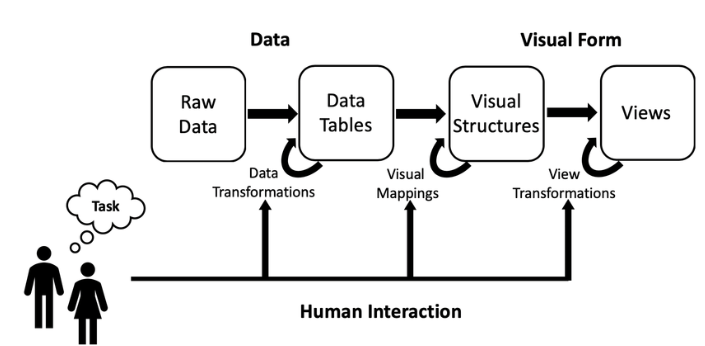
\includegraphics[width=0.75\linewidth]{figure/VizModelDiagram} 

}

\caption{Visual Reference model by Card}\label{fig:graphics}
\end{figure}

\db{While External Cognition describes the advances in graphical technology and how little had been done in the work of the cognitive framework of the discipline, the following citations by Ware attempt to develop the necessary guidelines that are useful for the work done by the perceptual experience.}

Colin Ware ``Information Visualization: Perception for Design'' (Ware, 2004) there are four stages of visualization

\begin{itemize}
\tightlist
\item
  The collection and storage of data itself
\item
  The preprocessing design to transform the data into something we can understand
\item
  The display hardware and the graphics algorithms produce the image on the screen.
\item
  The human perceptual and cognitive system
\end{itemize}

\db{The overlapping understanding in the field, while Ware takes the process one step further not just to allow the end user to understand the outcomes but to curate the outcomes with a visual perception of the data that makes the cognitive load easier for the end-user.}

\db{A dashboard has much information related to tabular data from multiple sources. 
Design should be recorded a produced with content that will allow for reproducibility. 
A dashboard should have some content related to interaction with the user. 
This interaction can be in multiple forms: toggling through the selection of variables to display uniformly to the use of interaction on the graph and allowing a user to understand best what is being shown in the diagram.}

\db{The entire dashboard/Interface should have a human perception piece that is useful for the user to comprehend and use. 
For example, the dashboard/interface could be more practical if the user is visually overwhelmed.}

\begin{itemize}
\tightlist
\item
  Identified the highly relevant from a dashboard design perspective (O'Donnell \& David, 2000)
\end{itemize}

\begin{enumerate}
\def\labelenumi{\arabic{enumi}.}
\tightlist
\item
  Information systems give interaction and feedback
\item
  Type of presentation format to be used
\item
  Differences in the amount of information load.
\end{enumerate}

Information load is essential, as dashboards must provide the right decision cues without overwhelming the user with excess information.

\db{"A decision cue is a feature of something perceived that is used in the interpretation of perception" [@choo2009],  where perception is an inferential process as objects in the environment can only be perceived indirectly through available information that has been sensed by the individual [@brunswik1952].}

\db{Visual complexity and information utility are required. 
Visual complexity refers to the "degree of difficulty in providing a verbal description of an image ([@heaps1999], [@olivia2004]).}

\begin{itemize}
\tightlist
\item
  Graphs are more suitable for spatial tasks (ex., for comparing a set of values) (Vessey \& Galletta, 1991);(Umanath \& Vessey, 1994);(Vessey, 1994)
\item
  Graphs reduced the negative influence of information overload
\item
  Graphs produced better correlation estimates and decreased time on a task (\textbf{schulzand?});(Booth \& Siegler, 2006)
\item
  Self-organizing maps and multidimensional scaling did not significantly outperform tabular representations (Huang et al., 2006)
\end{itemize}

The purposes of a dashboard:

\begin{enumerate}
\def\labelenumi{\arabic{enumi}.}
\tightlist
\item
  Consistency
\item
  Monitoring
\item
  Planning
\item
  Communication
\end{enumerate}

\db{Card stated "Use interactive visual representations of abstract, non-physically based data to amplify cognition." [@card1999]}

\db{Visual perception involves two elements - the perceptual and conceptual gist. 
The perceptual gist refers to the process of the brain when it determines the image properties that provide the structural representation of a scene, like color and texture. 
The conceptual gist refers to the scene's meaning, which is improved after the perceptual information is received ([@friedman1979]; [@olivia2004]).}

\db{Visual complexity might increase with the quality and range of objects and with varying material and surface styles [@heylighen1997].}

\db{Repetitive and uniform patterns and existing knowledge of the objects in the scene reduce visual complexity [@olivia2004].}

\db{If the guidelines on our visual information load can be related to statistical terminology, we can consider this the fisher information of visual information load. 
This load can be used as a metric for balancing the amount of information rather than overloading the consumer.}

Visual Data Mining

\db{For data mining to be effective, it is important to include humans in the data exploration process and combine the flexibility, creativity, and general knowledge of the computational power of today's computers. 
Visual data exploration aims at integrating humans in the data exploration process, applying their perceptual abilities to the large data sets available in today's computer systems [@kiem2002].}

The visual data exploration process can be seen as a hypothesis generation process:

\begin{itemize}
\tightlist
\item
  The visualizations of the data allow the user to gain insight into the data and come up with new hypotheses
\item
  Along with verification of the hypotheses
\end{itemize}

The main advantages of visual data exploration over automatic data mining techniques from statistics or machine learning are:

\begin{itemize}
\tightlist
\item
  visual data exploration can efficiently deal with highly inhomogeneous and noisy data.
\item
  visual data exploration is intuitive and requires no understanding of complex mathematical or statistical algorithms or parameters.
\end{itemize}

\db{Visual Exploration Paradigm, also known as MGV (Massive Graph Visualizer), is an integrated visualization and exploration system for massive multidigraph navigation [@abello2002]. 
MGV usually follows a three-step process:}

\begin{itemize}
\tightlist
\item
  overview first
\item
  zoom and filter
\item
  details-on-demand
\end{itemize}

\db{The user identifies interesting patterns and focuses on one or more of them. Note that visualization technology does not only provide the base visualization techniques for all three steps but also bridges the gap between the steps.}

Visualization Technique Classification:

\begin{itemize}
\tightlist
\item
  Standard 2D/3D displays such as bar charts and x-y plots
\item
  Geometrically transformed displays, such as landscapes and parallel coordinates, as used in a scalable framework
\item
  Icon-based displays such as needle icons and star icons as used in MGV
\item
  Dense pixel displays such as the recursive pattern and circle segments techniques and the graph sketches as used in MGV
\item
  Stacked displays, such as treemaps or dimensional stacking
\end{itemize}

Interaction and distortion techniques allow users to interact directly with the visualizations.

\begin{itemize}
\tightlist
\item
  Projection as used in the Grand Tour System
\item
  Filtering as used in Polaris
\item
  Zooming as used in MGV and scalable framework
\item
  Linking and Brushing as used in Polaris and the scalable framework
\end{itemize}

Design Theory in Information System

The knowledge is distinguished as the fifth of five types of theory:

\begin{enumerate}
\def\labelenumi{\arabic{enumi}.}
\tightlist
\item
  Analyzing \& describing
\item
  Understanding
\item
  Predicting
\item
  Explaining and predicting
\item
  Design and action
\end{enumerate}

\db{A definition of information systems that are suitable for our purposes concerns: "the effective design delivery use and impact of information technology in organizations and society [@avison1995]. }

The two paradigms characterize much of the research in the Information systems discipline:

\begin{itemize}
\tightlist
\item
  \emph{Behavioral Science Paradigm} - seeks to develop and verify theories that explain or predict human or organizational behavior (roots in natural science research methods).
\item
  \emph{Data Science Paradigm} - seeks to extend the boundaries of human and organizational capabilities by creating new and innovative artifacts (roots in engineering and the sciences of the artificial) (Simon, 1996).
\end{itemize}

\db{Technology and behavior are not dichotomous in an information system. They are inseparable [@lee2000]. Information technology (IT) artifacts are broadly defined as:}

\begin{itemize}
\tightlist
\item
  constructs (vocabulary \& symbols)
\item
  models (abstractions \& representations)
\item
  methods (algorithms \& practices)
\item
  instantiations (implemented \& prototype systems)
\end{itemize}

\db{These are concrete prescriptions that enable IT researchers and practitioners to understand and address the problems inherent in developing and successfully implementing information systems within organizations ([@march1995]; [@nunamaker1991]). }

Researchers have used PCPs to visualize categorical data.
Beygelzimer, Perng, Ma and Hellerstien created a fast ordering categorical data analysis algorithm that helped visualization, where their algorithms helped organize the original parallel coordinate plots clearer ((Beygelzimer, Perng, \& Ma, 2001); (Ma \& Hellerstein, 2001)).
Hammock plots are modified versions of similar coordinate plots invented by Schonlau to visualize categorical data (Schonlau, 2003).
His design replaces coordinate polygons with rectangles to present the number.
Treemaps are modified to support categorical data visualization.

\db{Exploratory Data Analysis (EDA) analyzes and summarizes a dataset to discover patterns, trends, and insights. 
It is a crucial step in the data analysis process and is often used to identify which variables are essential, what the data looks like, and what the underlying structure of the data is. 
EDA is typically done using various techniques, such as visualizations, statistical summaries, and data transformations.}

Mallows and Walley list psychology as one of four areas likely to support a theory of analysis Mallows \& Walley (1980).
Data analyses rely on the mind's ability to learn, analyze, and understand.

Visual inference uses our ability to detect graphical anomalies.
However, the idea of formal testing remains the same in visual inference -- with one exception: The test statistic is now a graphical display compared to a ``reference distribution'' of plots showing the null.

Data Scientists and other analytic professionals often use interactive visualization in the dissemination phase at the end of a workflow, during which findings are communicated to a wider audience.
Digital tools are critical to data science and analytics workflows, and current practice spans the following:

\begin{itemize}
\tightlist
\item
  \emph{Data Analysis Tools} - R, Pandas and SAS
\item
  \emph{Data Warehousing Services} - MySQL, MongoDB, or Amazon Redshift
\item
  \emph{Machine Learning Libraries} - scikit-learn o Apache MLlib
\end{itemize}

A typical process typically consists of the following general stages:

\begin{enumerate}
\def\labelenumi{\arabic{enumi}.}
\tightlist
\item
  \emph{Discovery}: Formulating an exciting question and determining the data necessary to answer it.
\item
  \emph{Acquisition}: Locating, organizing, and preparing data to be accessible to the chosen analysis environment.
\item
  \emph{Exploration}: Investigating and analyzing the data set to collect insights and understand the data
\item
  \emph{Modeling}: Building fitting and validating a model that can explain the data set and the observed phenomena
\item
  \emph{Communication}: Disseminating the results to stakeholders in reports, presentations, and charts.
\end{enumerate}

\hypertarget{variable-types}{%
\subsection{Variable Types}\label{variable-types}}

Not all variables should be used to create all types of charts - variable type informs chart structure
\db{
Categorical Data Visualization is the process of visualizing data that can be divided into distinct categories or groups. Categorical data are non-numeric and often represented by words, labels, or symbols, such as gender, product type, color, etc.}

\db{Visualizing categorical data helps uncover patterns and relationships between categories and can provide insights into the data distribution. 
Categorical data visualization techniques include bar charts, pie charts, histograms, stacked bar charts, and others. 
The choice of visual representation will depend on the data's nature and the insights being sought. 
The goal of categorical data visualization is to communicate the information effectively and make it easier to understand and interpret.}

\db{CatTree gives a hierarchical categorical data visualization with interaction [@kolatch2001]. 
Fernstad developed an interactive system combining parallel coordinates, tables, and scatterplot matrices for an overview explorative analysis. 
Thoroughly research categorical data visualization to support algorithm understanding. 
The novel contingency wheel presented by [@alsallakh2011] supports visual analytics in categorical data, and he measured association based on Pearson's residuals and used visual abstraction based on elements frequency.}

\db{High-Dimensional Data Visualization represents complex data sets with many variables or features (also known as high-dimensional data). 
The goal is to find effective ways to express such data in a form that allows easy understanding, analysis, and interpretation.
This is typically achieved by reducing the dimensionality of the data, for example, by projecting the data onto a lower-dimensional space or by aggregating the data in some way. 
The resulting visualizations can then reveal patterns, relationships, and other insights that would otherwise be difficult to detect from the raw data. 
For example, high-dimensional data visualization techniques include scatter plots, parallel coordinate plots, heat maps, and many others.}

\db{A popular research area in visualization since high-dimensional data is always fuzzy to mining. 
Direct visualization includes geometric visualizations:}

\begin{itemize}
\tightlist
\item
  scatterplots: use dots in coordinate to present data points.
\item
  parallel coordinates: present each dimension as axes, and every data item intersects dimensions as a polygon line at a particular position
\item
  RadViz/ PolyViz
\item
  GridViz
\end{itemize}

\db{Besides these traditional geometric visualization methods, iconographic displays like human faces and star glyphs used funny ways to present multivariate data. 
Hierarchical methods are used widely in parallel coordinates, which give analysts an intuitive view of clustering information [@fua1999]; [@johansson2005]. 
Rearrange the dimensions by dimension similarity on parallel coordinates, circle segments, and recursive patterns [@ankerst1998]. 
Guo used an interactive feature selection method to help users identify interesting subspaces from high-dimensional data sets [@guo2003].}

\db{Visualizations have become more effective in recent years due to the pandemic and the Johns Hopkins University COVID-19 Dashboard [@JHPHDashboard] [Dashboard](https://coronavirus.jhu.edu/map.html).
We were glued to our computers, TVs, and phones for most of the world. 
As a result, we watched the dashboard change in real-time to adapt to the users' needs. 
In part to data growth and changing, the dashboard, as well as the visualizations, were needed in a condensed platform. 
The need to be concise and vastly informative is a struggle regarding data visualizations. }

\db{Interactive visualization is a commonly used tool in Exploratory Data Analysis (EDA), which is the initial step in the data analysis process. 
The goal of EDA is to gain a high-level understanding of the data and to identify patterns, relationships, and anomalies in the data. }

The space of infographics has been a much better way of looking at data on a creative scale.(\textbf{stat?}\_graph\_hist)
While this may be a way of seeing the data in a friendly way, infographics need to include an interactive piece of data that many people would like to explore.

\hypertarget{multivariate-data-displays}{%
\subsection{Multivariate Data Displays}\label{multivariate-data-displays}}

\begin{itemize}
\tightlist
\item
  Difficulty of visualizing multivariate data
\item
  Different approaches - briefly mention

  \begin{itemize}
  \tightlist
  \item
    encoding with shape/color/etc.
  \item
    tours
  \item
    pcps
  \item
    linked graphics (interactivity)
  \end{itemize}
\end{itemize}

This section doesn't need to solve the problem - it just introduces it

Several methods can be used to conduct user analysis:

\begin{itemize}
\tightlist
\item
  Interviews: This involves conducting in-depth interviews with users to understand their needs, goals, and workflows.
\item
  Surveys involve sending out surveys to users to gather data on their needs and preferences.
\item
  Observations: This involves observing users as they complete tasks with the interface to understand their behaviors and workflows.
\item
  Personas: This is a method of creating fictional characters that represent the different types of users; it helps to understand the users' needs and goals.
\item
  Scenarios: This is a method of creating stories that describe how a user might interact with a system; it helps to understand the context and the user's needs.
\item
  Focus groups: This is a method of gathering a small group of users and facilitating a discussion to understand the users' needs and goals.
\item
  Contextual inquiry: This is a method of visiting the users in their work environment and observing them while they work; it helps to understand the context and the user's needs.
\end{itemize}

Several protocols and methods can be used to test the design of a dashboard or other visual display.
Some of these include:

\begin{itemize}
\tightlist
\item
  Usability testing: This involves having users interact with the dashboard and providing feedback on its usability, including how easy it is to navigate, understand, and use.
\item
  Cognitive walkthrough: This involves having experts in human-computer interaction evaluate the dashboard, focusing on the cognitive processes required to use it effectively.
\item
  Eye-tracking: This involves using technology to track the users' gaze and interactions, to understand the user's focus and attention on the dashboard elements.
\item
  A/B testing: This involves creating two versions of the dashboard, each with slightly different design elements, and comparing the results to see which design is more effective.
\item
  Surveys: This involves asking users to complete a survey that measures their satisfaction and understanding of the dashboard and to provide feedback on improvements.
\item
  Heat maps: This involves using heat maps to track where users are clicking on the dashboard to identify which elements are being used the most and which are being ignored.
\item
  Card sorting: This is a method to understand the users' mental models and how they would like to organize and categorize the data; it is helpful to understand how to structure the dashboard navigation.
\end{itemize}

\hypertarget{testing-graphics}{%
\chapter{Testing Graphics}\label{testing-graphics}}

\db{These are just a few examples of the many protocols and methods that can be used to test the design of a dashboard. 
The selection of the appropriate way will depend on the specific goals of the testing and the resources available. 
Remember that the user's feedback is crucial in the testing process; it will provide the necessary insight to improve the design and make it more efficient.}

Overview of testing methods for interactive graphics - talk aloud, measuring user engagement, etc.
\db{Testing interactive graphics using human perception principles in psychology involves considering various aspects of human perception and cognition to evaluate the effectiveness and user experience of the graphics. 
Here are some steps you can follow to test your interactive graphics:}

\db{Usability testing: Conduct a usability test to assess the ease of use and accessibility of the graphics. 
This includes testing for navigation, user control, and overall user experience.}

\db{Perception of visual elements: Evaluate how the visual elements in your graphics, such as color, contrast, size, and position, impact the perception of the information being presented.}

\db{Cognitive load: Assess the cognitive load on the user by evaluating how easily they can process and understand the information being presented. Factors such as complexity, amount of information, and type of information presented can impact cognitive load.}

\db{Attention allocation: Observe where the user's attention is directed while interacting with the graphics. This can help identify areas that may require improvement or modification to better engage the user's attention.}

\db{Memory retention: Evaluate the user's ability to retain and recall information presented in the graphics. This can help determine the effectiveness of the design in supporting memory retention.}

\db{User feedback: Obtain user feedback through surveys, interviews, or focus groups to gain insights into the user experience and identify areas for improvement.}

\db{It is important to keep in mind that human perception and cognition can vary greatly between individuals and can be influenced by a range of factors, such as age, culture, and personal experience. Testing with a representative sample of your target audience can help ensure that your interactive graphics are optimized for a wide range of users.}

\hypertarget{refs}{}
\begin{CSLReferences}{1}{0}
\leavevmode\vadjust pre{\hypertarget{ref-angel2000}{}}%
Angel, E. (2000). \emph{Interactive computer graphics : A top-down approach with OpenGL}. Boston, MA: Addison Wesley Longman.

\leavevmode\vadjust pre{\hypertarget{ref-angel2001}{}}%
Angel, E. (2001a). \emph{Batch-file computer graphics : A bottom-up approach with QuickTime}. Boston, MA: Wesley Addison Longman.

\leavevmode\vadjust pre{\hypertarget{ref-angel2002a}{}}%
Angel, E. (2001b). \emph{Test second book by angel}. Boston, MA: Wesley Addison Longman.

\leavevmode\vadjust pre{\hypertarget{ref-aspillaga1996}{}}%
Aspillaga, M. (1996). Perceptual foundations in the design of visual displays. \emph{Computers in Human Behavior}, \emph{12}(4), 587--600.

\leavevmode\vadjust pre{\hypertarget{ref-Bendix:2005}{}}%
Bendix, F., Kosara, R., \& Hauser, H. (2005). {Parallel Sets: Visual Analysis of Categorical Data}. In \emph{2005 IEEE symposium on information visualization (INFOVIS'05)} (pp. 133--140). IEEE. http://doi.org/\href{https://doi.org/10.1109/INFOVIS.2005.27}{10.1109/INFOVIS.2005.27}

\leavevmode\vadjust pre{\hypertarget{ref-beygelzimer2001}{}}%
Beygelzimer, A., Perng, C.-S., \& Ma, S. (2001). Fast ordering of large categorical datasets for better visualization. In \emph{Proceedings of the seventh ACM SIGKDD international conference on knowledge discovery and data mining} (pp. 239--244).

\leavevmode\vadjust pre{\hypertarget{ref-booth2006}{}}%
Booth, J. L., \& Siegler, R. S. (2006). Developmental and individual differences in pure numerical estimation. \emph{Developmental Psychology}, \emph{42}(1), 189.

\leavevmode\vadjust pre{\hypertarget{ref-cleveland1984}{}}%
Cleveland, W. S., \& McGill, R. (1984). Graphical perception: Theory, experimentation, and application to the development of graphical methods. \emph{Journal of the American Statistical Association}, \emph{79}(387), 531--554.

\leavevmode\vadjust pre{\hypertarget{ref-cowan2001}{}}%
Cowan, N. (2001). The magical number 4 in short-term memory: A reconsideration of mental storage capacity. \emph{Behavioral and Brain Sciences}, \emph{24}(1), 87--114.

\leavevmode\vadjust pre{\hypertarget{ref-dOcagne:1885}{}}%
d'Ocagne, M. (1885). {Coordonnées parallèles et axiales : Méthode de transformation géométrique et procédé nouveau de calcul graphique déduits de la considération des coordonnées parallèles}. \emph{Gauthier-Villars}, 112. Retrieved from \url{https://archive.org/details/coordonnesparal00ocaggoog/page/n10}

\leavevmode\vadjust pre{\hypertarget{ref-sine}{}}%
Day, R. H., \& Stecher, E. J. (1991). Sine of an illusion. \emph{Perception}, \emph{20}, 49--55.

\leavevmode\vadjust pre{\hypertarget{ref-dedonno}{}}%
DeDonno, M. A. (2016). The influence of IQ on pure discovery and guided discovery learning of a complex real-world task. \emph{Learning and Individual Differences}, \emph{49}, 11--16.

\leavevmode\vadjust pre{\hypertarget{ref-few}{}}%
Few, S. (2006). \emph{Information dashboard design: The effective visual communication of data}. Newton, MA: O'Reilly Media, Inc.

\leavevmode\vadjust pre{\hypertarget{ref-few2009}{}}%
Few, S. (2009). \emph{Now you see it: Simple visualization techniques for quantitative analysis}. Analytics Press.

\leavevmode\vadjust pre{\hypertarget{ref-density-pcp}{}}%
Heinrich, J., \& Weiskopf, D. (2009). {Continuous Parallel Coordinates}. \emph{IEEE Transactions on Visualization and Computer Graphics}, \emph{15}(6), 1531--1538. http://doi.org/\href{https://doi.org/10.1109/TVCG.2009.131}{10.1109/TVCG.2009.131}

\leavevmode\vadjust pre{\hypertarget{ref-ggpcp}{}}%
Hofmann, H., VanderPlas, S., \& Ge, Y. (2022). \emph{Ggpcp: Parallel coordinate plots in the ggplot2 framework}. Retrieved from \url{https://github.com/heike/ggpcp}

\leavevmode\vadjust pre{\hypertarget{ref-Hofmann:2013}{}}%
Hofmann, H., \& Vendettuoli, M. (2013). {Common Angle Plots as Perception-True Visualizations of Categorical Associations}. \emph{IEEE Transactions on Visualization and Computer Graphics}, \emph{19}(12), 2297--2305. http://doi.org/\href{https://doi.org/10.1109/TVCG.2013.140}{10.1109/TVCG.2013.140}

\leavevmode\vadjust pre{\hypertarget{ref-huang2006}{}}%
Huang, Z., Chen, H., Guo, F., Xu, J. J., Wu, S., \& Chen, W.-H. (2006). Expertise visualization: An implementation and study based on cognitive fit theory. \emph{Decision Support Systems}, \emph{42}(3), 1539--1557.

\leavevmode\vadjust pre{\hypertarget{ref-lee}{}}%
Lee, S., Kim, S.-H., Hung, Y.-H., Lam, H., Kang, Y., \& Yi, J. S. (2016). How do people make sense of unfamiliar visualizations?: A grounded model of novice's information visualization sensemaking. \emph{IEEE}, \emph{22}, 499--508.

\leavevmode\vadjust pre{\hypertarget{ref-luxen-vetter-2011}{}}%
Luxen, D., \& Vetter, C. (2011). Real-time routing with OpenStreetMap data. In \emph{Proceedings of the 19th ACM SIGSPATIAL international conference on advances in geographic information systems} (pp. 513--516). New York, NY, USA: ACM. http://doi.org/\href{https://doi.org/10.1145/2093973.2094062}{10.1145/2093973.2094062}

\leavevmode\vadjust pre{\hypertarget{ref-ma2001}{}}%
Ma, S., \& Hellerstein, J. L. (2001). Mining partially periodic event patterns with unknown periods. In \emph{Proceedings 17th international conference on data engineering} (pp. 205--214). IEEE.

\leavevmode\vadjust pre{\hypertarget{ref-mallows1980}{}}%
Mallows, C., \& Walley, P. (1980). A theory of data analysis. \emph{Proc. Amer. Statist. Assoc. Bus. Econ. Statist. Sec}, 8--14.

\leavevmode\vadjust pre{\hypertarget{ref-Molina1994}{}}%
Molina, S. T., \& Borkovec, T. D. (1994). The {P}enn {S}tate worry questionnaire: Psychometric properties and associated characteristics. In G. C. L. Davey \& F. Tallis (Eds.), \emph{Worrying: Perspectives on theory, assessment and treatment} (pp. 265--283). New York: Wiley.

\leavevmode\vadjust pre{\hypertarget{ref-elsi}{}}%
National Center for Education Statistics. (2020). National center for education statistics. \url{https://nces.ed.gov/}.

\leavevmode\vadjust pre{\hypertarget{ref-odonnell2000}{}}%
O'Donnell, E., \& David, J. S. (2000). How information systems influence user decisions: A research framework and literature review. \emph{International Journal of Accounting Information Systems}, \emph{1}(3), 178--203.

\leavevmode\vadjust pre{\hypertarget{ref-petersCommunityResiliencyDeclining2019}{}}%
Peters, David J. (2019). Community {Resiliency} in {Declining} {Small} {Towns}: {Impact} of {Population} {Loss} on {Quality} of {Life} over 20 {Years}. \emph{Rural Sociology}, \emph{84}(4), 635--668. http://doi.org/\href{https://doi.org/10.1111/ruso.12261}{10.1111/ruso.12261}

\leavevmode\vadjust pre{\hypertarget{ref-peters2018using}{}}%
Peters, David J., Hamideh, S., Zarecor, K. E., \& Ghandour, M. (2018). Using entrepreneurial social infrastructure to understand smart shrinkage in small towns. \emph{Journal of Rural Studies}, \emph{64}, 39--49.

\leavevmode\vadjust pre{\hypertarget{ref-Rlanguage}{}}%
R Core Team. (2021). \emph{R: A language and environment for statistical computing}. Vienna, Austria: R Foundation for Statistical Computing. Retrieved from \url{https://www.R-project.org/}

\leavevmode\vadjust pre{\hypertarget{ref-r}{}}%
R Core Team. (2022). \emph{R: A language and environment for statistical computing}. Vienna, Austria: R Foundation for Statistical Computing. Retrieved from \url{https://www.R-project.org/}

\leavevmode\vadjust pre{\hypertarget{ref-reedweb2007}{}}%
Reed~College. (2007). LaTeX your document. Retrieved from \url{http://web.reed.edu/cis/help/LaTeX/index.html}

\leavevmode\vadjust pre{\hypertarget{ref-scc}{}}%
Rural Shrink Smart Team. (2022). Rural shrink smart. \url{https://ruralshrinksmart.org/}.

\leavevmode\vadjust pre{\hypertarget{ref-fisher}{}}%
Sarikaya, A., Correll, M., Bartram, L., Tory, M., \& Fisher, D. (2019). What do we talk about when we talk about dashboards? \emph{IEEE Transactions on Visualization and Computer Graphics}, \emph{25}(1), 682--692. http://doi.org/\href{https://doi.org/10.1109/TVCG.2018.2864903}{10.1109/TVCG.2018.2864903}

\leavevmode\vadjust pre{\hypertarget{ref-schonlau2003}{}}%
Schonlau, M. (2003). Visualizing categorical data arising in the health sciences using hammock plots. In \emph{Proceedings of the section on statistical graphics, american statistical association}.

\leavevmode\vadjust pre{\hypertarget{ref-schulz2013}{}}%
Schulz, H.-J., Nocke, T., Heitzler, M., \& Schumann, H. (2013). A design space of visualization tasks. \emph{IEEE Transactions on Visualization and Computer Graphics}, \emph{19}(12), 2366--2375.

\leavevmode\vadjust pre{\hypertarget{ref-simon1996}{}}%
Simon, H. A. (1996). The sciences of the artificial 3rd ed. \emph{MIT Press Cambridge}.

\leavevmode\vadjust pre{\hypertarget{ref-iowa_gov}{}}%
State of Iowa. (2020). Iowa data portal. \url{https://data.iowa.gov}.

\leavevmode\vadjust pre{\hypertarget{ref-umanath1994}{}}%
Umanath, N. S., \& Vessey, I. (1994). Multiattribute data presentation and human judgment: A cognitive fit perspective. \emph{Decision Sciences}, \emph{25}(5-6), 795--824.

\leavevmode\vadjust pre{\hypertarget{ref-Rural_classification}{}}%
USDA - ERS. (2020a). Rural classifications. \url{https://www.ers.usda.gov/topics/rural-economy-population/rural-classifications/}.

\leavevmode\vadjust pre{\hypertarget{ref-usda}{}}%
USDA - ERS. (2020b). Rural-urban commuting area codes. \url{https://www.ers.usda.gov/data-products/rural-urban-commuting-area-codes/}.

\leavevmode\vadjust pre{\hypertarget{ref-sineillusion}{}}%
VanderPlas, S., \& Hofmann, H. (2015a). Signs of the sine illusion--why we need to care. \emph{Journal of Computational and Graphical Statistics}, \emph{24}(4), 1170--1190. http://doi.org/\href{https://doi.org/10.1080/10618600.2014.951547}{10.1080/10618600.2014.951547}

\leavevmode\vadjust pre{\hypertarget{ref-vanderplas2015}{}}%
VanderPlas, S., \& Hofmann, H. (2015b). Signs of the sine illusion---why we need to care. \emph{Journal of Computational and Graphical Statistics}, \emph{24}(4), 1170--1190.

\leavevmode\vadjust pre{\hypertarget{ref-vessey1994}{}}%
Vessey, I. (1994). The effect of information presentation on decision making: A cost-benefit analysis. \emph{Information \& Management}, \emph{27}(2), 103--119.

\leavevmode\vadjust pre{\hypertarget{ref-vessey1991}{}}%
Vessey, I., \& Galletta, D. (1991). Cognitive fit: An empirical study of information acquisition. \emph{Information Systems Research}, \emph{2}(1), 63--84.

\leavevmode\vadjust pre{\hypertarget{ref-Ware2004}{}}%
Ware, C. (2004). \emph{Information visualization: Perception for design}. San Francisco, CA: Morgan Kaufmann Publisher.

\leavevmode\vadjust pre{\hypertarget{ref-ware2012}{}}%
Ware, C. (2012). \emph{Information visualization: Perception for design}. Morgan Kaufmann.

\leavevmode\vadjust pre{\hypertarget{ref-ggplot2}{}}%
Wickham, H. (2016). \emph{{ggplot2: Elegant Graphics for Data Analysis}} (2nd ed.). Springer-Verlag New York. Retrieved from \url{https://ggplot2.tidyverse.org}

\leavevmode\vadjust pre{\hypertarget{ref-tourr}{}}%
Wickham, H., Cook, D., Hofmann, H., \& Buja, A. (2011). {tourr: An R Package for Exploring Multivariate Data with Projections}. \emph{Journal of Statistical Software, Articles}, \emph{40}(2), 1--18. http://doi.org/\href{https://doi.org/10.18637/jss.v040.i02}{10.18637/jss.v040.i02}

\leavevmode\vadjust pre{\hypertarget{ref-zarecor2021rural}{}}%
Zarecor, K. E., Peters, D. J., \& Hamideh, S. (2021). Rural smart shrinkage and perceptions of quality of life in the american midwest. In \emph{Handbook of quality of life and sustainability} (pp. 395--415). Springer.

\end{CSLReferences}


%% backmatter is needed at the end of the main body of your thesis to
%% set up page numbering correctly for the remainder of the thesis
\backmatter

%% Start the correct formatting for the appendices
% \appendix
%% Input each appendix here
% \input{./appendix_a}

%% Bibliography goes here (You better have one)
%% BibTeX is your friend

% \bibliographystyle{alpha}  % or use  abbrv to abbreviate first names and use numerical indices
\bibliographystyle{abbrv}  % or use  abbrv to abbreviate first names and use numerical indices
%% Add your BibTex file here (don't include the .bib)
\bibliography{./references}



%% Index go here (if you have one)
\end{document}
